\documentclass[a4paper,11pt]{article}
\usepackage[english]{babel}
\usepackage[utf8]{inputenc}
\usepackage[T1]{fontenc}
\usepackage{graphicx}
\usepackage{amsmath}
\usepackage{tikz}
\usepackage{amsthm}
\usepackage{amssymb}
\usepackage{nicefrac}
\usepackage{cprotect}
\usepackage{wrapfig}
\usepackage{framed}
\usepackage{fancyvrb}
\usepackage{bm}
\usepackage{fvextra}
\usepackage{listings}
\usepackage{mathtools}
\usepackage{mhchem}
\usepackage{longtable}
\usepackage[nottoc,numbib]{tocbibind}
\usepackage[left=25mm,right=25mm,bottom=25mm,top=25mm]{geometry} %left, right, bottom ,top, includeheadfoot
\usepackage{caption}
\usepackage{multicol}
\usepackage{subcaption}
\usepackage[framemethod=TikZ]{mdframed}
\usepackage{nameref}
\usepackage{placeins} %Put command \floatbarrier in front of textpassage or other items, in front of which the desired content (i.e. images) shall be placed.
\usepackage{titlesec}
\usepackage[inline]{enumitem}
% \usepackage[parfill]{parskip}
%\usepackage{fancyhdr}
\usepackage{enumitem}
\usepackage{siunitx}
\newcounter{question}
\setcounter{question}{0}
\usepackage{blindtext}
\usepackage{hyperref} %To make document linked within.
\usepackage{cleveref}
\numberwithin{equation}{section}
\captionsetup{font=footnotesize,labelfont=bf}

\renewcommand{\theenumi}{(\arabic{enumi})}
\renewcommand\labelenumi{\theenumi} % Change enumerate style from 1. to (1) etc.
\renewcommand{\theenumiii}{(\arabic{enumiii})}
\renewcommand\labelenumiii{\theenumiii} % Change enumerate style from 1. to (1) etc.
\setlist{itemsep = 0.2pt}


\newcommand\matr[1]{\ensuremath{\boldsymbol{\mathbf{#1}}}}
\newcommand\vect[1]{\ensuremath{\bm{#1}}}
\newcommand\dint{\ensuremath{\int\displaylimits}}

%\DeclareSIUnit \parsec {pc}
%\DeclareSIUnit \magnitudes {mag}

\title{General Relativity\\ \vspace{0.2cm}\normalsize Questions and answers}
\author{Daniel Zahnd}
\date{\today}

 \newmdenv[backgroundcolor = lightgray!40, roundcorner = 0pt, linewidth = 0pt]{greybox}

\newtheorem{ass}{Assertion}

%%%%%%%%%%%%%%%%%%%%%%%%%%%%%%%%%%%%%%%%%%
%
% See book of Atmospheric Science of Wallace
% and Hobbs for explanations
% (or Andrews and Achatz)
%
%%%%%%%%%%%%%%%%%%%%%%%%%%%%%%%%%%%%%%%%%%
\begin{document}


\newcommand\Que[1]{%
   \leavevmode\par
   \stepcounter{question}
   \noindent
   \thequestion. \textbf{Q} --- #1\par}

\newcommand\Ans[2][]{%
    \leavevmode\par\noindent
   {\leftskip0pt
    \textbf{A} --- \textbf{#1}#2\par}}

\maketitle
\thispagestyle{empty}
\tableofcontents

\newpage

\pagenumbering{arabic}
\setcounter{page}{1}

\section{Special relativity}
\Que{How is th notation of special relativity and also of general relativity characterized?}
\Ans{
Special relativity (SR) may be formulated by means of so-called four-vectors $x^\mu$.
A four-vector is defined as \begin{equation}\label{defvierervektor}
x^\mu = (x^0 = ct,x^k) = (x^0,x^1,x^2,x^3) = (x^0, \vect{x}),
\end{equation} where $c$ denotes the speed of light and $t$ refers to the time in an inertial system. Greek letters $(\mu, \nu, \dots)$ are used for the components of four-vectors, latin letters $(i,j,\dots)$ for general vectors of euclidean space.

A Matrix $A$ is written as $A_{\mu\nu}$, where the Einstein sum convenction is applicable. Summation therefore is understood to take place over two identical indices, where one index is a subscript and one a superscript. For example, the multiplication of a $n\times m$-matrix $A$ with a $n\times 1$-vector $v$ is written as \begin{equation}
w = Av \quad \Leftrightarrow \quad w^\mu =\sum_{\nu = 1}^{m}A^\mu_{\nu} v^\nu \equiv A^\mu_{\nu} v^\nu,
\end{equation} where \begin{enumerate}
\item summation always runs over two identical indices, whereof one is sub- and the other superscripted,
\item $(A^\mu_{\nu})^T = (A^\nu_{\mu})$ holds,
\item $(A^\mu_{\nu})^{-1} = (A_\mu^{\nu})$ holds in addition and also
\item the row rumbers are positioned as superscripts and the column numbers are positioned as subscripts.
\end{enumerate}
}

\Que{What is an inertial reference system? What considerations give rise to special relativity?}
\Ans{
An intertial frame is a reference frame, which moves with none or constant speed relative to the fixed stars and is therefore not accelerated relative to those fixed stars.
The principle of relativity by Galilei holds, that \begin{enumerate*}
\renewcommand{\theenumi}{(G\arabic{enumi})}
\renewcommand\labelenumi{\theenumi}\item \label{Galileo1} all inertial systems are equivalent\footnote{That means, that in all inertial systems the same physical principles apply.} and that \item \label{Galileo2} Newton's axioms hold in all inertial systems.
\end{enumerate*} The principle of relativity by Einstein however holds that \begin{enumerate*}
\renewcommand{\theenumi}{(E\arabic{enumi})}
\renewcommand\labelenumi{\theenumi}\item \label{Einstein1} all inertial systems are equivalent and \item \label{Einstein2} in all inertial systems the speed of light is isotropically constant and equal to $c$.
\end{enumerate*}

Empirical properties of light are incompatible with Galilei's principle of relativity \ref{Galileo1} and \ref{Galileo2}, but undoubtedly compatible with Einstein's principle of relativity \ref{Einstein1} and \ref{Einstein2}.
In order to find a correct transformation rule for physical entities from one inertial system to another, the invariance of the wave operator \begin{equation}
\Box = -\frac{1}{c^2}\frac{\partial^2}{\partial t^2} + \Delta = \eta^{\mu\nu}\partial_\mu\partial_\nu
\end{equation} under the transformation $x^\mu \rightarrow \bar{x}^\mu$ may be demanded, where $\Delta = \vect{\nabla}^2$ is the laplacian. The reason for this heuristic approach is that light can be described by the wave equation, which may be expressed by the box operator $\Box$. Einstein's principle \ref{Einstein2} demands the isotropic invariance of light in inertial systems, therefore the invariance of the wave operator $\Box$ is a plausible claim in oder to find a correct transformation between intertial systems. This claim leads to the so-called Poincaré- and Lorentz-transformations.
}

\Que{How is Minkowski space defined?}
\Ans{
In analogy to the common, euclidean space, the so-called Minkowski space is a real space $\mathbb{R}^4$ equipped by the Minkowski metric $d_M$. The Minkowski metric is defined as \begin{equation}
d_M: \mathbb{R}^4 \times \mathbb{R}^4 \rightarrow \mathbb{R}, \quad (x^\mu,x^\nu) \mapsto \eta_{\mu\nu}x^\mu x^\nu,
\end{equation} where $\eta_{\mu\nu} = \mathrm{diag}(-1,+1,+1,+1)$ (\flqq mostly-plus\frqq\ convention) is the Minkowski tensor with $\eta_{\mu\nu}\eta^{\nu\kappa} = \delta_\mu^{\kappa}$. The Minkowski space is then given by the tuple $(\mathbb{R}^4,d_M)$.

The Minkowski line element $\mathrm{d}s^2$ in Minkowski space is given by \begin{equation}
\mathrm{d}s^2 = \eta_{\mu\nu}\,\mathrm{d}x^\mu\,\mathrm{d}x^\nu.
\end{equation}

The gradient $\partial_\mu$ in the space of four-vectors is a so-called covariant Lorentz vector. In the above mentioned notation it holds that \begin{equation}\label{diffoplower}
\partial_\mu = \frac{\partial}{\partial x^\mu} = \left(\frac{\partial}{\partial x^0},\frac{\partial}{\partial x^1},\frac{\partial}{\partial x^2},\frac{\partial}{\partial x^3} \right) = \left(\frac{1}{c}\frac{\partial}{\partial t}, \vect{\nabla}\right).
\end{equation} For the corresponding contravariant Lorentz vector $\partial^\mu$ the relation \begin{equation}\label{diffopupper}
\partial^\mu = \eta^{\mu\nu}\partial_\nu = \left(\frac{1}{c}\frac{\partial}{\partial t},-\vect{\nabla}\right)
\end{equation} is valid.
}

\Que{What are Poincaré and Lorentz transformations and how are they defined and derived?}
\Ans{
A transformation law \begin{equation}
L:(\mathbb{R}^4,d_M) \rightarrow (\mathbb{R}^4,d_M), \quad x^\mu \mapsto \bar{x}^\mu = L^\mu_{\nu}x^\nu + b^\mu, \quad b_\mu = \text{const.} \in \mathbb{R}^4
\end{equation} is a Poincaré transformation if and only if $L$ leaves the Minkowski line element $\mathrm{d}s$ invariant under this transformation: \begin{equation}
\eta_{\mu\nu}\bar{x}^\mu\bar{x}^\nu = \eta_{\mu\nu}x^\mu x^\nu \quad \Leftrightarrow \quad \eta_{\mu\nu} L^\mu_{\kappa}L^\nu_{\delta} = \eta_{\kappa \delta} \quad \Leftrightarrow \quad \matr{L}^T\matr{\eta} \matr{L} = \matr{\eta}.
\end{equation} These class of functions describe transformations between intertial systems of arbitrary physical entities expressed in four-vectors. The invariance of the Minkowski line element $\mathrm{d}s$ and the invariance of the wave operator $\Box$ under Lorentz transformations are equivalent.

Let there be two inertial systems $\Sigma$ and $\bar{\Sigma}$, where the inertial system $\bar{\Sigma}$ shall move with constant speed $\vect{v}=(v,0,0)$ relative to $\Sigma$. The goal now is to find a transformation between those inertial systems, which fullfills Einstein's axioms \ref{Einstein1} and \ref{Einstein2}. The fullfillement of these axioms is equivalent with the invariance of the wave operator $\Box$ under the sought-after transformation. Einstein's axioms lead to the following requirements for the sought-after transformations:
\begin{enumerate}
\item From Einstein's axiom \ref{Einstein1} it follows that the sought-after transformation equations must be linear, since if there were quadratic terms in space $\vect{x}$ or time $t$, then derivatives with respect to space or time would still be dependent on space and/or time. Because of the requirement of equivalence of all inertial systems this must not be the case - this is, because equivalence of all inertial systems means that the physical laws must be of the same shape in all inertial systems.
\item From Einstein's axiom \ref{Einstein2} the requirement of constant speed of light follows, aswell as the
\item requirement, that the sought-after transformation prescription transitions to a Galilei transformation for $v \ll c$.
\end{enumerate}
If the notation $x^\mu = (ct,x^1,x^2,x^3)$ is applied for coordinates in the inertial system $\Sigma$ and $\bar{x}^{\mu} = (c\bar{t},\bar{x}^{1},\bar{x}^{2},\bar{x}^{3})$ for coordinates in the inertial system $\bar{\Sigma}$, it follows from the third above requirement, that \begin{equation}\label{eq:bedlor1}
(x^1)^2+(x^2)^2+(x^3)^2 = c^2 \cdot t^2 \quad \Leftrightarrow \quad (\bar{x}^{1})^2+(\bar{x}^{2})^2+(\bar{x}^{3})^2 = c\cdot \bar{t}^{\,2}
\end{equation} must hold. This follows directly from a consideration of a light flash, whose wavefront propagates spherically. The first and the second requirement yield the following Ansatz for the sought-after transformation law:
\begin{equation}
\bar{x}^\mu = \begin{pmatrix}
c \bar{t} \, \\ \bar{x}^1 \\ \bar{x}^2 \\ \bar{x}^3
\end{pmatrix} = \begin{pmatrix}
c (Bx^1 +  Dt) \\ A(x^1-vt) \\ x^2 \\ x^3
\end{pmatrix}, \quad A,B,D \in \mathbb{R}.
\end{equation} Inserting this Ansatz in the equations of condition \eqref{eq:bedlor1}, the values for the coefficients $A$, $B$ and $D$ follow as \begin{equation}
A = \gamma, \quad B = -\frac{\beta}{c}\gamma, \quad D = \gamma,\end{equation} where the beta and the gamma factors are defined by \begin{equation} \beta = \frac{v}{c}, \quad \gamma = \frac{1}{\sqrt{1-\beta^2}}.
\end{equation} Herewith the transformation may be written as \begin{equation}
\bar{x}^\mu = \begin{pmatrix}
c \bar{t}\, \\ \bar{x}^1 \\ \bar{x}^2 \\ \bar{x}^3
\end{pmatrix} = \begin{pmatrix}
-\beta \gamma x^1 + c \gamma t \\ \gamma (x^1-vt) \\ x^2 \\ x^3
\end{pmatrix} = \begin{pmatrix}
\gamma c t - \beta \gamma x^1 \\ -\beta \gamma c t + \gamma x^1 \\ x^2 \\ x^3
\end{pmatrix},
\end{equation} with $v = \beta c $. The defined transformation $\bar{x}^\mu = L^\mu_{\nu} x^\nu$ can be represented with the expression \begin{equation}
\bar{x}^\mu = \begin{pmatrix}
c\bar{t} \\ \bar{x}^1 \\ \bar{x}^2 \\ \bar{x}^3
\end{pmatrix} = L^\mu_{\nu} x^\nu = \underbrace{\begin{pmatrix}
\gamma & -\beta\gamma & 0 & 0 \\
-\beta\gamma & \gamma & 0 & 0 \\
0 & 0 & 1 & 0 \\
0 & 0 & 0 & 1
\end{pmatrix}}_{= \, L^\mu_{\nu}}\underbrace{\begin{pmatrix}
ct \\ x^1 \\ x^2 \\ x^3
\end{pmatrix}}_{= \, x^\nu} = \begin{pmatrix}
\gamma ct - \beta\gamma x^1 \\ -\beta\gamma ct + \gamma x^1 \\ x^2 \\ x^3
\end{pmatrix},
\end{equation} where the (1,1)-tensor $L^\mu_{\nu}$ was used, which can in turn be written in matrix form in the case at hand. It can be mathematically shown, that $L^\mu_{\nu}$ satisfies the relation \begin{equation}
\eta_{\mu\nu} L^\mu_{\kappa}L^\nu_{\delta} = \eta_{\kappa \delta}
\end{equation} and must therefore be a Lorentz transformation. With the special Lorentz transformation defined by $L \doteq L^\mu_{\nu}$ in the coordinates $(x^0=ct, x^1)$, arbitrary transformations $\mathcal{T}$ between inertial systems can be described. Herewith rotations $R$ in the coordinates $\vect{x} = (x^1,x^2,x^3)$, translations $T$ in the coordinates $x^\mu = (x^0=ct,x^1,x^2,x^3)$ and special Lorentz transformations $L$ in the coordinates $(x^0 = ct, x^1)$ must be executed in a chain. Therefore, for an arbitrary transformation from one inertial system to another, the definition equation for such a transformation can be written as \begin{equation}
\mathcal{T} = L \circ R \circ T \quad \Leftrightarrow \quad \bar{x}^\mu = \mathcal{T}(x^\mu) = (L\circ T \circ R)(x^\mu) = L(R(T(x^\mu))).
\end{equation}
}

\Que{How are proper time and eigenspace defined?}
\Ans{
Let $x^\mu$ and $\bar{x}^\mu$ be the same worldline of a massive particle in different inertial systems $\textrm{IS}$ and $\overline{\textrm{IS}}$. In the moving systems $\overline{\textrm{IS}}$ the differential of the four-vector $\bar{x}^\mu$ takes the form $\mathrm{d}\bar{x}^\mu = (c\,\mathrm{d}\bar{t},0,0,0)$, therefore the Minkowski line element is given as $\mathrm{d}\bar{s}^{\,2} = \eta_{\mu\nu}\,\mathrm{d}\bar{x}^\mu\,\mathrm{d}\bar{x}^\nu = -c^2\,\mathrm{d}\bar{t}^{\,2} \doteq -c^2\,\mathrm{d}\tau^2.$
Because of invariance under Lorentz transformations it holds that \begin{equation}
\mathrm{d}\bar{s} = \mathrm{d}s \quad \Leftrightarrow \quad -c^2\mathrm{d}\tau^2 = -c^2\mathrm{d}t^2 + (\mathrm{d}x^1)^2 + (\mathrm{d}x^2)^2 + (\mathrm{d}x^3)^2 = -c^2(\mathrm{d}t)^2 + (\mathrm{d}\vect{x})^2.
\end{equation} For a differential $(\mathrm{d}q)^n$ the notation $\mathrm{d}q^n \equiv (\mathrm{d}q)^n, n \in \mathbb{N}$ is usually applied. From this it follows that \begin{equation}
\vect{v}(t) = \frac{\mathrm{d}\vect{x}(t)}{\mathrm{d}t} \quad \Rightarrow \quad \mathrm{d}\tau^2 = \mathrm{d}t^2-\frac{(\mathrm{d}\vect{x})^{2}}{c^2} \quad \Leftrightarrow \quad \mathrm{d}\tau = \mathrm{d}t\,\sqrt{1-\frac{\vect{v}(t)^2}{c^2}} = \gamma(\vect{v})^{-1}\mathrm{d}t
\end{equation} holds, where $\gamma(\vect{v}) = (1-\nicefrac{\vect{v}(t)^2}{c^2})^{-\nicefrac{1}{2}} = (1-\beta(\vect{v})^2)^{-\nicefrac{1}{2}}$ is the gamma factor. The integral \begin{equation}
\tau_{PQ} = \int\displaylimits_{\tau_P}^{\tau_Q} \, \mathrm{d}\tau = \int\displaylimits_{t_P}^{t_Q} \sqrt{1-\frac{\vect{v}(t)^2}{c^2}} \,\mathrm{d}t
\end{equation} is called proper time (eigentime).

In a very analogous way the differential of the four vector $\bar{x}^\mu$ in the moving system $\overline{\textrm{IS}}$ takes the form $\mathrm{d}\bar{x}^\mu = (0,\mathrm{d}\bar{x}^1,\mathrm{d}\bar{x}^2,\mathrm{d}\bar{x}^3)$. Therefore the Minkowski line element is written as $\mathrm{d}\bar{s}^{\,2} = \eta_{\mu\nu}\,\mathrm{d}\bar{x}^\mu\,\mathrm{d}\bar{x}^\nu = (\mathrm{d}\bar{x}^1)^2+(\mathrm{d}\bar{x}^2)^2+(\mathrm{d}\bar{x}^3)^2 = (\mathrm{d}\bar{\vect{x}})^2$. Because of invariance under Lorentz transformations again the relation \begin{equation}
\mathrm{d}\bar{s} = \mathrm{d}s \quad \Leftrightarrow \quad (\mathrm{d}\bar{\vect{x}})^2 = -c^2\mathrm{d}t^2 + (\mathrm{d}x^1)^2 + (\mathrm{d}x^2)^2 + (\mathrm{d}x^3)^2 = -c^2(\mathrm{d}t)^2 + (\mathrm{d}\vect{x})^2
\end{equation} holds. From this the validity of \begin{equation}
\vect{v}(t) = \frac{\mathrm{d}\vect{x}(t)}{\mathrm{d}t} \quad \Rightarrow \quad \mathrm{d}\bar{s}^{\,2} = -c^2\,\mathrm{d}t^2+(\mathrm{d}\vect{x})^2 \quad \Leftrightarrow \quad \mathrm{d}\bar{s} = \mathrm{d}t\,\sqrt{\vect{v}(t)^2-c^2}.
\end{equation} follows. The integral \begin{equation}
s_{PQ} = \int\displaylimits_{P}^{Q} \, \mathrm{d}\bar{s} = \int\displaylimits_{t_P}^{t_Q}\,\mathrm{d}t\,\sqrt{\vect{v}(t)^2-c^2}
\end{equation} is the called eigenspace.
}

\Que{How are the four-position, the four-velocity, the four-acceleration and the four-momentum defined?}
\Ans{
By means of proper time $\tau$ a Lorentz invariant time parameter is given, which is therefore a very natural choice to parametrize wordlines $x^\mu(t)$ with. The four-position is given as \begin{equation}\label{viererposition}
x^\mu(t) \doteq (ct,\vect{x}(t)), \quad x_\mu x^\mu = \eta_{\mu\nu}x^\mu x^\nu = -ct^2 + \vect{x}^{\,2}.
\end{equation} The four-velocity $u^\mu(\tau)$ is given as the derivative of the four-position with respect to proper time by \begin{equation}\label{vierergeschwindigkeit}
u^\mu(\tau) \doteq \frac{\mathrm{d}x^\mu(\tau)}{\mathrm{d}\tau} = (\gamma(\vect{v})c,\gamma(\vect{v})\vect{v}), \quad u_\mu u^\mu = \eta_{\mu\nu}u^\mu u^\nu = -c^2.
\end{equation} The four-acceleration $a^\mu(\tau)$ is accordingly given as the second derivative of the four-position with respect to proper time by \begin{equation}\label{viererbeschleunigung}
a^\mu(\tau) \doteq \frac{\mathrm{d}^2x^\mu(\tau)}{\mathrm{d}\tau^2}.
\end{equation} The four-momentum $p^\mu(\tau)$ is then naturally defined by multiplying the mass of a particle with the four-velocity, such that \begin{equation}\label{viererimpuls}
p^\mu(\tau) \doteq mu^\mu(\tau) = m\frac{\mathrm{d}x^\mu(\tau)}{\mathrm{d}\tau} = m(\gamma(\vect{v})c,\gamma(\vect{v})\vect{v}), \quad p_\mu p^\mu = m^2\eta_{\mu\nu}u^\mu u^\nu = -m^2c^2
\end{equation} holds, where the four-momentum can also be written as \begin{equation}
p^\mu(\tau) = (E/c, \vect{p}),
\end{equation} since $mc^2\gamma(\vect{v})$ is the relativistic energy of a massive particle. Calculating the dot product \begin{equation}
p_\mu p^\mu = m^2\eta_{\mu\nu}u^\mu u^\nu = -m^2c^2 = -\frac{E^2}{c^2} + \vect{p}^{\,2} \quad \Leftrightarrow \quad E^2 = \vect{p}^{\,2}c^2 + m^2c^4
\end{equation} the well-known energy-momentum relation follows, which is sometimes called the \flqq Massenschale\frqq\ in German.
}

\Que{What is the light cone of an event and how are timelike, spacelike and lightlike distances defined? Which implications concerning causality are there?}
\Ans{
Consider the Minkowski line element $\mathrm{d}s^2 = \eta_{ab}\,\mathrm{d}x^a\,\mathrm{d}x^b$ for some coordinates $x^\mu = (ct, x^1, x^2)$ in three-dimensional spacetime, which is short of one dimension as compared to the real four-dimensional case. Now, the worldlines of light in this space can be described by means of a light cone as shown in \cref{fig:lightcone}.
\begin{figure}[h]
	\centering
	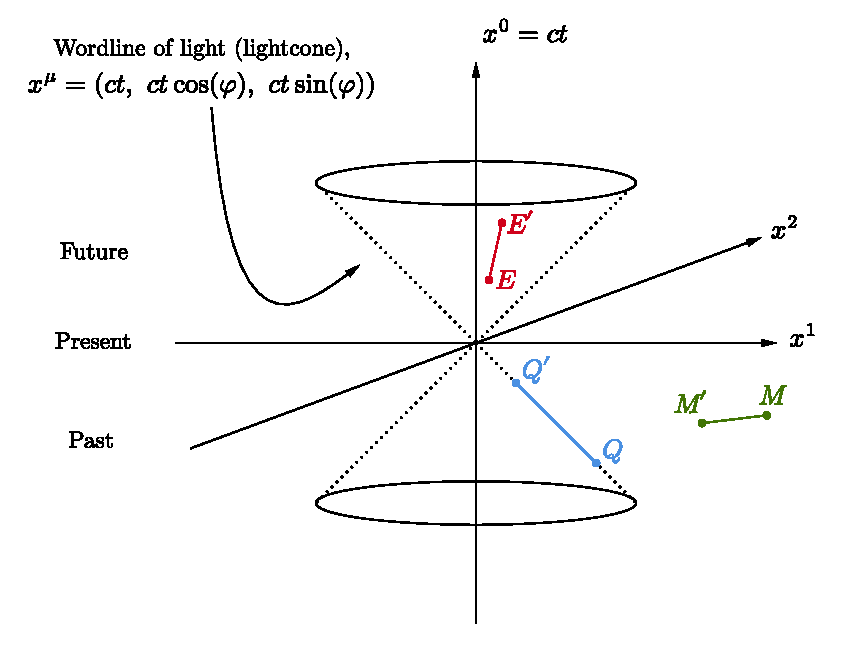
\includegraphics[width=0.6\textwidth]{figures/lightcone.pdf}
	\caption{Visualization of a light cone in three-dimensional Minkowski spacetime.}
	\label{fig:lightcone}
\end{figure}
Now, let $d^a$ be the connecting vector between two events in Minkowski spacetime, defined as \begin{equation}
	d^a = (c(t^\prime-t),x^{1\,\prime}-x^{1}, x^{2\,\prime}-x^{2}),
\end{equation} where the non-primed quantities are associated to event 1 and the primed quantities to event 2. Depending on the sign of $d^a$ in this case (or of the Minkowski line element $\mathrm{d}s^2$ in the general case), one gives this vector the name lightlike (null), spacelike or timelike.

The vector $d^a$ is called \textit{lightlike}, if $\eta_{ab}d^a d^b = 0$ (or $\mathrm{d}s^2 = 0$ in the general case). That is to say that two events $Q$ and $Q^\prime$ are situated on the light cone. This corresponds to the situation, where information travels at the speed of light; therefore $Q$ and $Q^\prime$ can be causally connected, if the causal connection ``travels'' at the speed of light.

The vector $d^a$ is called \textit{spacelike}, if $\eta_{ab}d^a d^b > 0$ (or $\mathrm{d}s^2 > 0$ in the general case). That is to say that two events $M$ and $M^\prime$ are situated not within the light cone. This corresponds to the situation, where information travels at more than the speed of light; therefore, $M$ and $M^\prime$ cannot be causally connected.

The vector $d^a$ is called \textit{timelike}, if $\eta_{ab}d^a d^b < 0$ (or $\mathrm{d}s^2 < 0$ in the general case). That is to say that two events $E$ and $E^\prime$ are situated on the light cone. This corresponds to the situation, where information travels at speeds below the speed of light; therefore $E$ and $E^\prime$ can be causally connected. 
 % Question 2.3 on klassische Feldtheorie notes
}

\section{Action principle and Noether's theorem}
\Que{What is the action principle and how is it formulated in the most general case?}
\Ans{
Consider the most general case, where one has fields $\Phi^A(x^a)$, which can have more than one coordinate $A \in \{0,1,2,\dots\}$ and can depend on more than one coordinate $a \in \{0,1,2,\dots\}$.

The Lagrangian of a system is defined as a quantity, if integrated over all space $x^a$ gives the action $S[\Phi]$ of a system described by a field $\Phi^A(x^a)$. It depends on the field itself, on derivatives to arbitrary order of the field and explicitly also on the spacetime coordinates $x^a$, so \begin{equation}
L = L(\Phi^A, \partial_a \Phi^A, \dots, x^a), \quad \partial_a = \frac{\partial}{\partial x^a}, \quad \Phi^A = \Phi^A(x^a).
\end{equation} Therefore, the action of such a Lagrangian is defined as 
\begin{equation}
S[\Phi] = \int_{\mathbb{R}^D} L(\Phi^A, \partial_a \Phi^A, \dots, x^a)\,\mathrm{d}^Dx, \quad D \in \mathbb{N},
\end{equation} where $D$ is the dimension of the considered spacetime.

The action principle states, that whenever the Euler-Lagrange equations are satisfied, the action is stationary, i.e. $\delta S[\Phi] = 0$. The Euler-Lagrange equations describe the equations of motion for an arbitrary system.

\begin{ass}[General action principle]
Consider a Lagrangian $L(\Phi^A, \partial_a \Phi^A, x^a)$, where $\Phi^A = \Phi^A(x^a)$. Whenever the Euler-Lagrange equations \begin{equation}
\left(\frac{\partial L}{\partial \Phi^A}-\frac{\mathrm{d}}{\mathrm{d}x^a}\frac{\partial L}{\partial(\partial_a \Phi^A)}\right) = 0
\end{equation} are satisfied, the action $S[\Phi]$ becomes stationary, i.e. $\delta S[\phi] = 0$ under a variation $\Phi^A \rightarrow \Phi^A + \delta \Phi^A$.
\end{ass}
\begin{proof}
Consider the variation $\Phi^A \rightarrow \Phi^A + \delta \Phi^A$. Now, the variation of the action $S[\Phi]$ is calculated as 
\begin{align}
\begin{aligned}
\delta S[\Phi] &= \delta \int_{\mathbb{R}^d} L(\Phi^A,\partial_a\Phi^A, x^a)\,\mathrm{d}^Dx = \int_{\mathbb{R}^d} \delta L(\Phi^A,\partial_a\Phi^A, x^a)\,\mathrm{d}^Dx.
\end{aligned}
\end{align} The variation $\delta L$ of the Lagrangian can be obtained by means of \begin{align}
\begin{aligned}
\delta L &= \frac{\partial L}{\partial \Phi^A}\delta \Phi^A + \frac{\partial L}{\partial(\partial_a \Phi^A)}\delta (\partial_a\Phi^A) \\
&= \frac{\partial L}{\partial \Phi^A}\delta \Phi^A + \frac{\mathrm{d}}{\mathrm{d}x^a}\left(\frac{\partial L}{\partial(\partial_a\Phi^A)}\right)\delta \Phi^A - \frac{\mathrm{d}}{\mathrm{d}x^a}\left(\frac{\partial L}{\partial(\partial_a\Phi^A)}\right)\delta \Phi^A + \frac{\partial L}{\partial(\partial_a \Phi^A)}\delta (\partial_a\Phi^A) \\
&= \left(\frac{\partial L}{\partial \Phi^A}-\frac{\mathrm{d}}{\mathrm{d}x^a}\frac{\partial L}{\partial(\partial_a\Phi^A)}\right)\delta \Phi^A + \frac{\mathrm{d}}{\mathrm{d}x^a}\left(\frac{\partial L}{\partial(\partial_a\Phi^A)}\delta \Phi^A\right).
\end{aligned}
\end{align} Inserting this expression into the above integral yields \begin{align}
\begin{aligned}
\delta S[\Phi] &= \int_{\mathbb{R}^d} \delta L(\Phi^A,\partial_a\Phi^A, x^a)\,\mathrm{d}^Dx \\
&=  \int_{\mathbb{R}^d} \underbrace{\left(\frac{\partial L}{\partial \Phi^A}-\frac{\mathrm{d}}{\mathrm{d}x^a}\frac{\partial L}{\partial(\partial_a\Phi^A)}\right)}_{=\,0}\delta \Phi^A \,\mathrm{d}^Dx + \underbrace{\int_{\mathbb{R}^d} \frac{\mathrm{d}}{\mathrm{d}x^a}\left(\frac{\partial L}{\partial(\partial_a\Phi^A)}\delta \Phi^A\right)\,\mathrm{d}^Dx}_{=\,\frac{\partial L}{\partial(\partial_a\Phi^A)}\delta\Phi^A \big|_{\partial \mathbb{R}^D}=0} = 0,
\end{aligned}
\end{align} because the variations $\delta \Phi^A$ at the boundary of the integration space are required to vanish and the Euler-Lagrange equations are assumed to be satisfied. Thus the action is stationary as shown.
\end{proof}

 % What is an action, what is a Lagrangian, how is it derived.
}

\Que{How is the Noether theorem stated and derived in the most general case?}
\Ans{ Noether's theorem states, that any symmetry in a system has a conserved quantity associated to it. Hence, for a variation $\Phi^A \rightarrow \Phi^A + \Delta \Phi^A$ denoting some symmetry, there is an associated conserved quantity associated to this symmetry.
\begin{ass}[Noether theorem]
Let $L(\Phi^A, \partial_a \Phi^A, x^a)$ be a Lagrangian with $\Phi^A = \Phi^A(x^a)$. A variation $\Delta \Phi^A \rightarrow \Phi^A + \Delta \Phi^A$ which leaves the Lagrangian invariant up to a total derivative, i.e. \begin{align}\begin{aligned}
\Delta L &= \left(\frac{\partial L}{\partial \Phi^A}-\frac{\mathrm{d}}{\mathrm{d}x^a}\frac{\partial L}{\partial(\partial_a\Phi^A)}\right)\Delta \Phi^A + \frac{\mathrm{d}}{\mathrm{d}x^a}\left(\frac{\partial L}{\partial(\partial_a\Phi^A)}\Delta \Phi^A\right) \\
&= \frac{\mathrm{d}}{\mathrm{d}x^a}F^a_{\Delta}(\Phi^A, x^a),
\end{aligned}\end{align} will give rise to a conserved current \begin{equation}
J_\Delta^a = \frac{\partial L}{\partial(\partial_a\Phi^A)}\Delta \Phi^A- F^a_{\Delta}
\end{equation} for any solution of the Euler-Lagrange equations.
\end{ass}
\begin{proof}
Consider the variation of the action \begin{align}
\begin{aligned}
\Delta S[\Phi] &= \int_{\mathbb{R}^3} \left(\frac{\partial L}{\partial \Phi^A}-\frac{\mathrm{d}}{\mathrm{d}x^a}\frac{\partial L}{\partial(\partial_a\Phi^A)}\right)\Delta \Phi^A  \,\mathrm{d}^3x + \int_{\mathbb{R}^D} \frac{\mathrm{d}}{\mathrm{d}x^a}\left(\frac{\partial L}{\partial(\partial_a\Phi^A)}\Delta \Phi^A\right)   \,\mathrm{d}^D x \\
&= \int_{\mathbb{R}^D} \frac{\mathrm{d}}{\mathrm{d}x^a}F^a_{\Delta}(\Phi^A, x^a) \,\mathrm{d}^Dx.
\end{aligned}
\end{align} Since the Euler-Lagrange equations are required to be satisfied, the first integral is zero, hence the equation \begin{align}
\begin{aligned}
\int_{\mathbb{R}^D} \frac{\mathrm{d}}{\mathrm{d}x^a}\left(\frac{\partial L}{\partial(\partial_a\Phi^A)}\Delta \Phi^A - F^a_{\Delta}\right)   \,\mathrm{d}^D x = \int_{\mathbb{R}^D} \frac{\mathrm{d}}{\mathrm{d}x^a}J^a_\Delta \,\mathrm{d}^Dx = 0
\end{aligned}
\end{align} can be derived from the above one, where the notation $F^a_\Delta = F^a_\Delta (\Phi^A,x^a)$ was used. In order for the above integral to be satisfied, the equation \begin{equation}
\frac{\mathrm{d}}{\mathrm{d}x^a}J^a_\Delta = 0
\end{equation} needs to hold, which is exactly what is claimed by the Noether theorem.
\end{proof}
}

% See Fliessbach chapter 14


\section{Einstein equivalence principle: From gravity to geometry}

\Que{What are the basic two equations of Newton's theory of gravity? How may they be described? Why can they not describe a full theory of gravity?}
\Ans{
One of the two basic equations of Newton's gravity describes the motion of a particle in a given gravitational field described by $\phi$. It is the well known equation of motion \begin{equation}
m\ddot{\vect{x}} = \vect{F}_g = -m\vect{\nabla}\phi.
\end{equation} The other equation describes the dynamics of the gravitational field itself. This is the also well known Poisson equation given by \begin{equation}
\Delta \phi = 4\pi G_N\mu,
\end{equation} which determines how the gravitational field $\phi$ is to be determined from $\mu$. The field $\phi$, the force $\vect{F}_g$ aswell as the mass density $\mu$ depend on the space coordinates $\vect{x} = \vect{x}(t)$.

It is evident that these equations cannot feasibly yet describe a complete theory of relativity - this is firstly because the operator $\Delta = \vect{\nabla}^2$ is not Lorentz invariant, secondly, because a change in the mass density at some point in space will immediately lead to a change in the gravitational field $\phi$ everywhere in space, which is almost not conceivable, since that would mean that information about a change in the mass density would travel faster than light, which contradicts known fundamental laws of physics.
}

\Que{What are the concepts of \textit{intertial mass} $m_i$ and \textit{gravitational mass} $m_g$? What is empirically so special about them?}
\Ans{
The concepts of inertial mass $m_i$ and $m_g$ arise from the newtonian equation of motion \begin{equation}
m_i \ddot{\vect{x}} = \vect{F}_g = -m_g\vect{\nabla}\phi,
\end{equation} where $m_i$ denote the \textit{inertial mass} and $m_g$ the \textit{gravitational mass}. For comparison reasons, the equation of motion for a particle with electric charge $q_e$ in an electrostatic field $\vect{E} = -\vect{\nabla}\phi_e$ reads \begin{equation}
m_i\ddot{\vect{x}} = -q_e\vect{\nabla}\phi_e.
\end{equation} From the electrostatic case of this equation it becomes evident, that there is no good reaston to assume a priori $m_g = m_i$. The left hand side of the newtonian equation of motion describes the resistance of a particle with mass $m_i$ against acceleration, while the right hand side accounts for the coupling of the \flqq gravitational charge\frqq\ $m_g$ to the gravitational field $\phi$.

The inertial mass is a measure for the resistance of a particle against accelerations, whereas the gravitational mass is a measure for the coupling of the particle's mass to the gravitational field. The surprising fact about $m_i$ and $m_g$ is that they are experimentally found to be equal to one another, so (locally) $m_i = m_g$ holds.
}

\Que{What are the \textit{elevator thought experiments} and which three key facts can be learned from them?}
\Ans{
The elevator thought experiments are thought experiments by Einstein intended to show the equivalence of inertial and gravitational mass. There are 

The basic setup of these thought experiments is to consider an experimenter in a sealed box (elevator) \flqq dropping\frqq\ two stones, one from the outstretched left hand and one from the outstretched right hand.

\begin{enumerate}
\item \label{elevthought1}Consider the elevator in outer space in the absence of any forces. If the experimenter now drops the stones, they will float just as the experimenter himself.
\item \label{elevthought2} Consider the elevator in outer space accelerated by a constant acceleration in the upward direction from the point of view of the experimenter. The experimenter aswell as the stones will then be pressed to the bottom of the elevator.
\item \label{elevthought3} Consider the elevator brought into a constant gravitational field. The experimenter aswell as the dropped stones will then again be pressed to the bottom of the elevator.
\item \label{elevthought4} Consider the elevator being dropped while residing in a constant gravitational field. The experimenter aswell as the dropped stones will then again be floating around the elevator.
\end{enumerate}

Firstly, it can be learned from thought experiments \ref{elevthought2} and \ref{elevthought3}, that locally the effects due to acceleration or gravity are indistinguishable.

Secondly, from \ref{elevthought3} and \ref{elevthought4} one may learn, that the effect of gravity can locally be eliminated by switching to a freely falling reference frame. Since situation \ref{elevthought1} and \ref{elevthought4} do not differ from the point of view of the experimenter, we must conclude that $m_i = m_g$ holds. If $m_i = m_g$ did not hold, then the experimenter in situation \ref{elevthought3} would observe a different behaviour from situation \ref{elevthought1} and the stones would either move upwards or downwards in the elevator. The gravitational field accelerates proportional to the gravitational mass $m_g$, while the object resists the gravitational acceleration proportional to the inertial mass $m_i$.

Thirdly, from observations in situation \ref{elevthought1} to \ref{elevthought4} we can learn, that the effect of a gravitational field in an arbitrary gravitational field cannot be eliminated globally by switching to a freely falling coordinate system - this is only possible in uniform and constant gravitational fields. But locally, it is possible. Consider the hanging elevator for example in a spherically symmetric gravitational field, such as that of the earth. The stones inside the elevator will be observed to drop down to the floor, moving slightly towards one another, since they move towards the center of the gravitational potential. Thus, the elimination of the gravitational effects by means of switching coordinate systems is possible only locally in a non-uniform gravitational field, this is why the term \flqq locally\frqq\ in the above text is important.
}

\Que{How may the Einstein equivalence principle be formulated and what does it mean?}
\Ans{
The Einstein equivalence principle may be stated as follows:
\begin{quote}
At every spacetime point in an arbitrary gravitational field it is possible to choose a locally inertial coordinate system such that within a sufficiently small region of this point, the laws of nature take the same form as in unaccelerated cartesian cordinate systems in the absence of gravitation.
\end{quote}

This equivalence principle states essentialy, that the inertial mass $m_i$ is the same as the gravitational mass $m_g$. With reference to the elevator thought experiment this principle says, that the experimenter inside a freely falling elevator placed in a constant gravitational field observes the same laws of nature as an experimenter inside an elevator which is floating in outer space with zero gravitational force acting upon the elevator.

Two interesting insights following directly from the equivalence principle in combination with special relativity are the following:
\begin{enumerate}
\item Light is deflected by a gravitational field just like material objects.
\item Clocks run slower in a gravitational field than in the absence of gravity.
\end{enumerate}
The first insight arises considering the following thought experiment. Consider a rocket accelerating at a constant acceleration rate. Furthermore, consider a relatively to the rocket unaccelerated light ray entering a window to the left of the rocket and exiting at the right of the rocket. The light ray will evidently be bent downwards since it will exit the rocket at a lower point of the rocket than it entered into the rocket. By the equivalence priniciple, which states that gravitational acceleration ist just like any other acceleration to a massive particle, it follows with special relativity that the gravitational field deflects light, because special relativity accounts for the deflection of light in accelerated systems. The second insight follows from the so-called \flqq twin-paradox\frqq\ in special relativity which essentially states that clocks in unaccelerated (inertial) systems run faster than clocks in accelerated systems. Since the gravitational field exerts acceleration on a massive particle, gravitation is to be considered as acceleration and therefore clocks will run slower in the presence of gravitation than they run in the absence of any gravitational forces.
}

\Que{What are pseudo-forces concerning the motion of particles in a gravitational field? Wherewith or why do they arise?}
\Ans{
Consider a four-vector $x^\mu(\tau)$ describing the position of a massive particle. The equation of motion for this particle ist given as \begin{equation}
m_i\frac{\mathrm{d}^2x^\mu(\tau)}{\mathrm{d}\tau^2} = F^\mu,
\end{equation} where $m_i$ is the inertial mass and $F^\mu$ is a four-vector describing the force accelerating the particle. If one performs a coordinate transformation \begin{equation}
x^\mu(\tau) \rightarrow z^\nu(x^\mu),
\end{equation} the derivatives with respect to proper time transform as
\begin{equation}
\dot{z}^\nu = \frac{\mathrm{d}z^\nu(x^\mu(\tau))}{\mathrm{d}\tau} = \underbrace{ \frac{\partial z^\nu}{\partial x^\mu}}_{=\,J^\nu_{\mu}}\frac{\mathrm{d}x^\mu}{\mathrm{d}\tau} = J^\nu_{\mu} \dot{x}^\mu
\end{equation} and \begin{gather}
\begin{gathered}
\ddot{z}^\nu = \frac{\mathrm{d}^2z^\nu(x^\mu(\tau))}{\mathrm{d}\tau^2} = \frac{\mathrm{d}}{\mathrm{d}\tau}\left(\frac{\partial z^\nu}{\partial x^\mu}\dot{x}^\mu\right) = \frac{\partial z^\nu}{\partial x^\mu}\ddot{x}^\mu + \dot{x}^\mu\frac{\partial }{\partial x^\lambda}\frac{\partial z^\nu}{\partial x^\mu}\frac{\mathrm{d}x^\lambda}{\mathrm{d}\tau} \\ = \underbrace{\frac{\partial z^\nu}{\partial x^\mu}}_{=\,J^\nu_{\mu}}\ddot{x}^\mu + \frac{\partial^2 z^\nu}{\partial x^\lambda \partial x^\mu}\dot{x}^\lambda \dot{x}^\mu = J^\nu_{\mu}\ddot{x}^\mu + \frac{\partial^2 z^\nu}{\partial x^\lambda \partial x^\mu}\dot{x}^\lambda \dot{x}^\mu.
\end{gathered}\end{gather} Then the equation of motion $m_i \ddot{x}^\mu = F^\mu$ transforms as \begin{equation}
m_i \ddot{z}^\nu = m_i J^\nu_{\mu}\ddot{x}^\mu + m_i\frac{\partial^2 z^\nu}{\partial x^\lambda \partial x^\mu}\dot{x}^\lambda \dot{x}^\mu = J^\nu_{\mu}F^\mu + P^\nu, \quad P^\nu = m_i \frac{\partial^2 z^\nu}{\partial x^\lambda \partial x^\mu}\dot{x}^\lambda \dot{x}^\mu.
\end{equation} The term $P^\nu$ is called a pseudo-force\footnote{A pseudo-force is a force which can be eliminated, if the system is transformed to an inertial reference frame.} and arises because of the coordinate transformation $x^\mu \rightarrow z^\nu(x^\mu)$ from an inertial to a non-inertial reference frame. Since the equivalence principle states $m_i = m_g$, this term scales linearly with the gravitational mass.
}

\Que{How may a potential for pseudo-forces be found and specified?}
\Ans{
We consider the equation of motion \begin{equation}
m_i \ddot{x}^\mu = 0
\end{equation} of a free particle in an inertial system with coordinates $x^\mu(\tau)$ and transform it to an accelerated system with coordinates $z^\nu(x^\mu) \overset{\text{Not.}}{=} z^\nu(x)$. In general, for a transformation $x^\mu(\tau) \leftrightarrow z^\nu(x^\mu)$ the relations \begin{equation}
\frac{\mathrm{d}}{\mathrm{d}\tau}x^\mu = \frac{\partial x^\mu}{\partial z^\nu}\frac{\mathrm{d}z^\nu}{\mathrm{d}\tau}, \quad \frac{\mathrm{d}}{\mathrm{d}\tau}z^\nu = \frac{\partial z^\nu}{\partial x^\mu}\frac{\mathrm{d}x^\mu}{\mathrm{d}\tau}
\end{equation} hold. Therefore, we have for the second derivatives \begin{equation}
\frac{\mathrm{d}^2}{\mathrm{d}\tau^2}x^\mu = \ddot{x}^\mu = \frac{\mathrm{d}}{\mathrm{d}\tau}\left(\frac{\partial x^\mu}{\partial z^\nu}\frac{\mathrm{d}z^\nu}{\mathrm{d}\tau}\right)= \frac{\partial x^\mu}{\partial z^\nu}\ddot{z}^\nu + \frac{\partial^2 x^\mu}{\partial z^\nu\partial z^\lambda}\dot{z}^\nu \dot{z}^\lambda \end{equation} and \begin{equation}
\frac{\mathrm{d}^2}{\mathrm{d}\tau^2}z^\nu = \ddot{z}^\nu = \frac{\mathrm{d}}{\mathrm{d}\tau}\left(\frac{\partial z^\nu}{\partial x^\mu}\frac{\mathrm{d}x^\mu}{\mathrm{d}\tau}\right)= \frac{\partial z^\nu}{\partial x^\mu}\ddot{x}^\mu + \frac{\partial^2 z^\nu}{\partial x^\mu\partial x^\lambda}\dot{x}^\mu \dot{x}^\lambda.
\end{equation} Assuming the Jacobi matrices \begin{equation}
J^\mu_{\nu}(z) = \frac{\partial x^\mu}{\partial z^\nu} \quad \text{and} \quad J^\nu_{\mu}(x) = \frac{\partial z^\nu}{\partial x^\mu}
\end{equation} have an inverse everywhere such that \begin{equation}
J^\mu_{a}(z)J_\mu^{b}(z) = \delta_a^{b}, \quad J_\mu^{a}(z)J^\mu_{b}(z) = \delta_{b}^{a}, \quad J^\nu_{a}(x)J_\nu^{b}(x) = \delta_a^{b}, \quad J_\nu^{a}(x)J^\nu_{b}(x) = \delta_{b}^{a}
\end{equation} holds, we do with $\ddot{x}^\mu$ some further manipulations, namely
\begin{align}
\begin{aligned}
\ddot{x}^\mu =&\; \frac{\partial x^\mu}{\partial z^\nu}\ddot{z}^\nu + \frac{\partial^2 x^\mu}{\partial z^\nu}\dot{z}^\nu \dot{z}^\lambda = J^\mu_{b}(z) \ddot{z}^b + \delta^\mu_{a}\frac{\partial^2 x^a}{\partial z^\nu\partial z^\lambda}\dot{z}^\nu \dot{z}^\lambda \\ =&\; J^\mu_{b}(z) \ddot{z}^b + \underbrace{J^\mu_{b}(z)J_a^{b}(z)}_{=\, \delta^\mu_{a}} \frac{\partial^2 x^a}{\partial z^\nu\partial z^\lambda}\dot{z}^\nu \dot{z}^\lambda = J^\mu_{b}(z)\left(\ddot{z}^b + J_a^{b}(z)\frac{\partial^2 x^a}{\partial z^\nu \partial z^\lambda}\dot{z}^\nu \dot{z}^\lambda \right) = 0.
\end{aligned} \end{align} The jacobian $J^\mu_{b}(z)$ must be nonzero, because it is assumed to have an inverse, hence the equation of motion \begin{equation}
\ddot{z}^b + J_a^{b}(z)\frac{\partial^2 x^a}{\partial z^\nu \partial z^\lambda}\dot{z}^\nu \dot{z}^\lambda  = \ddot{z}^b + \underbrace{\frac{\partial x^b}{\partial z^a}\frac{\partial^2 x^a}{\partial z^\nu \partial z^\lambda}}_{\doteq \, \gamma^b_{\nu \lambda}}\dot{z}^\nu \dot{z}^\lambda = \ddot{z}^\nu + \gamma^\nu_{\kappa \lambda} \dot{z}^\kappa \dot{z}^\lambda = 0
\end{equation} results for $z^\nu$ in the accelerated system.

To summarize, for a transformation $x^\mu \rightarrow z^\nu(x)$ from an inertial system to an arbitrarily accelerated system the relation \begin{equation}
m_i\ddot{x}^\mu = 0 \quad  \xrightarrow{x^\mu \rightarrow z^\nu(x)} \quad m_i\ddot{z}^\nu = -m_i\gamma^\nu_{\kappa\lambda}\dot{z}^\kappa \dot{z}^\lambda = -m_g\gamma^\nu_{\kappa\lambda}\dot{z}^\kappa \dot{z}^\lambda
\end{equation} holds, where the last equation follows from the equivalence principle $m_i = m_g$. Comparing this equation to the Newtonian equation of motion \begin{equation}
m_i \ddot{\vect{x}} = -m_g\vect{\nabla}\phi,
\end{equation} we see that there is given some equivalence: \begin{equation}
\vect{\nabla}\phi \quad \text{is somehow equivalent to} \quad \gamma^\nu_{\kappa\lambda}\dot{z}^\kappa \dot{z}^\lambda.
\end{equation} Since by the Einstein equivalence principle one can locally not distinguish between general acceleration or acceleration due to a gravitational field, the transformation $x^\mu \rightarrow z^\nu(x)$ can well be understood as a transformation of a free particle to a reference frame in a gravitational field, where the term $-m_g\gamma^\nu_{\kappa\lambda}\dot{z}^\kappa \dot{z}^\lambda$ arises due to the gravitational potential. It is possible to show, that $\gamma^\nu_{\kappa \lambda}$ is related to the metric of spacetime - so the gravitational potential or gravity, if you will, is essentially determined by the geometry of spacetime! The quantity $\gamma^\nu_{\kappa \lambda}$ is actually made up of derivatives of the metric of spacetime and provides exactly 10 \flqq potentials\frqq.\

For some general metric space $y^\mu$ equipped with a metric $g_{\mu\nu}=g_{\mu\nu}(y)$, the above equations look like \begin{equation}
m_i \ddot{y}^\mu + m_g\Gamma^\mu_{\nu\lambda}\dot{y}^\nu\dot{y} = 0,
\end{equation} where $\Gamma^\mu_{\nu\lambda}$ are the Christoffel symbols defined as \begin{equation}
\Gamma^{\mu}_{\nu\lambda} = g^{\mu\rho}\Gamma_{\rho\nu\lambda} = g^{\mu\rho}\frac{1}{2}\left(g_{\rho\nu,\lambda} + g_{\rho\lambda,\nu}-g_{\nu\lambda,\rho}\right).
\end{equation} Therefore, the term $\vect{\nabla}\phi$ in the classical formulation is equivalent to $\Gamma^\mu_{\nu\lambda}\dot{y}^\nu\dot{y}$ and is therefore related to the metric $g_{\mu\nu}(y)$ of the metric space. Therefore, the effect of gravity can be described by a suitable metric on the considered space.
}

\Que{What does it mean, when an object is called ``freely falling'' in general relativity?}
\Ans{
In the context of general relativity, the term ``freely falling'' means that an object described with this term is only subject to gravitation and no other forces or influences. Then, general relativity states that such freely falling objects move along geodesics in spacetime.
}

\section{Metrics, geometry and geodesics}
\Que{Given some coordinates $x^a$ with associated metric $f_{ab}=f_{ab}(x)$ and new coordinates $y^\mu(x)$ with associated metric $g_{\mu\nu}=g_{\mu\nu}(y)$; how does the metric $f_{ab}$ transform to the new metric $g_{\mu\nu}$, if it is required, that the proper distances stay invariant?}
\Ans{
Let $x^a$ be the former coordinates with associated metric $f_{ab}(x)$, and let $y^\mu(x^a)$ be the new coordinates with associated metric $g_{\mu\nu}(y)$. The proper distances in each coordinates is given by the metric multiplied by an infinitesimal space element, namely $\mathrm{d}s^2(x) = f_{ab}\,\mathrm{d}x^a\,\mathrm{d}x^b$ and $\mathrm{d}s^2(y) = g_{\mu\nu}\,\mathrm{d}y^\mu\,\mathrm{d}y^\nu$; hence, the condition that the proper distance stay invariant would require $\mathrm{d}s^2(x) = \mathrm{d}s^2(y)$ and it just means, that distances do not depend on the choice of coordinate system.

Consider the space element $\mathrm{d}y^\mu = \frac{ \partial y^\mu}{\partial x^a}\,\mathrm{d}x^a$. With that relation, we can formulate \begin{align}\begin{aligned}
g_{\mu\nu}\,\mathrm{d}y^\mu\,\mathrm{d}y^\nu &= g_{\mu\nu}\frac{ \partial y^\mu}{\partial x^a}\frac{ \partial y^\nu}{\partial x^b}\,\mathrm{d}x^a\,\mathrm{d}x^b = \underbrace{g_{\mu\nu}J^\mu_{a}(x)J^\nu_{b}(x)}_{\doteq f_{ab}}\,\mathrm{d}x^a\,\mathrm{d}x^b = f_{ab}\,\mathrm{d}x^a\,\mathrm{d}x^b,
\end{aligned}\end{align} where the Jacobi matrices \begin{equation}
J^\mu_{a} = J^\mu_{a}(x) \doteq \frac{\partial y^\mu(x)}{\partial x^a} \quad \text{and}\quad J^a_{\mu} = J^a_{\mu}(y) \doteq \frac{\partial x^a(y)}{\partial y^\mu}
\end{equation} have been defined. As one sees, the condition that proper distance stays constant in all coordinate systems requires the metrics to transform as \begin{equation}
f_{ab}(x) = g_{\mu\nu}(y)J^\mu_{a}(x)J^\nu_{b}(x) = g_{\mu\nu}J^\mu_{a}J^\nu_{b} \doteq g_{\mu\nu}(x).
\end{equation} In terms of matrix multiplications, this condition can also be written as \begin{equation}
\matr{f} = \matr{J}^T \matr{g} \matr{J},
\end{equation} where $\matr{f} = f_{ab}$, $\matr{J}^T = (J^\mu_{a})^T = J^a_{\mu}$ and $\matr{g} = g_{\mu\nu}$ was used.
}

\Que{How can a non-degenerate and symmetric metric be defined on some spacetime space and what properties does it have?}
\Ans{
Let $\mathbb{R}^4$ be spacetime equipped with some metric $g_{\mu\nu}(x)$, describing, how distances are measured in coordinates $x^\mu$. That is, the line element $\mathrm{d}s^2(x)$ in the $x^\mu$ coordinates is defined as \begin{equation}
\mathrm{d}s^2(x) = g_{\mu\nu}(x)\,\mathrm{d}x^\mu\,\mathrm{d}x^\nu
\end{equation} and does not depend on the choice of coordinate system. Since different metrics can define the same geometry, there is in this case a coordinate transformation $x^\mu \rightarrow y^a$ to some other coordinates. The metric $g_{\mu\nu}(x)$ transforms in this case to the new coordinates as \begin{equation}
g_{ab}(y) = g_{\mu\nu}(x)\frac{\partial x^\mu}{\partial y^a}\frac{\partial x^\nu}{\partial y^b} = g_{\mu\nu}(x)J^\mu_{a}(y)J^\nu_{b}(y),
\end{equation} such that \begin{equation}
g_{\mu\nu}(x)\,\mathrm{d}x^\mu\,\mathrm{d}x^\nu = g_{ab}(y)\,\mathrm{d}y^a\,\mathrm{d}y^b
\end{equation} holds.

In general, non-degeneracy and symmetry is assumed for a metric $g_{\mu\nu}(x)$, that is \begin{equation}
g_{\mu\nu}(x) = g_{\nu\mu}(x) \quad \text{and} \quad \det\left[g_{\mu\nu}(x)\right]
\end{equation} hold. This means, that there is an inverse metric for every metric defined in such a manner. Consider the following remarks:
\begin{enumerate}
\item The inverse metric is denoted with upper indices, that is the inverse of $g_{\mu\nu}(x)$ is $g^{\mu\nu}(x)$. Therefore, $g^{\mu\nu}(x)g_{\nu\lambda}(x) = \delta^\mu_{\lambda}$ holds.
\item spacetime equipped with a metric tensor $g_{\mu\nu}(x)$ is called a metric spacetime in the general case. If all eigenvalues of the metric are positive, then one calls the space Riemannian spacetime, if one eigenvalue is negative and three eigenvalues are positive, one speaks of a pseudo-Riemannian spacetime or of a Lorentzian spacetime.
\end{enumerate}
}

\Que{How do the eigenvalues of the Minkowski metric look like? What is special about the Minkowski metric compared to other metrics?}
\Ans{
Consider a vector $\vect{v} \in \mathbb{R}^4$ and let the Minkowski metric $\eta_{ab}$ in mostly-plus convention be written as a matrix $\matr{\eta} = \eta_{ab}$. The eigenvalue condition is given by \begin{equation}
\matr{\eta}\vect{v} = \lambda \vect{v} \quad \Leftrightarrow \quad \det\left[\matr{\eta}-\lambda \matr{E}\right],
\end{equation} where $\matr{E}$ is the four-dimensional unity matrix. This equation leads to the characteristic polynome \begin{equation}
(-1-\lambda)(1-\lambda)^3 = 0,
\end{equation} which results in the eigenvalues $\lambda_1 = -1$ and $\lambda_{2,3,4}= 1$. So the Minkowski metric has one negative and three positive constant eigenvalues, therefore $\mathbb{R}^4$ equipped with the Minkowski metric is considered a pseudo-Riemannian or Lorentzian spacetime. This is precisely what is special about the Minkowski metric - it has constant eigenvalues, namely one negative and three positive eigenvalues, which are all 1 in terms of magnitude.
}

\Que{How are the Christoffel symbols defined?}
\Ans{
The Christoffel symbols of the first kind $\Gamma_{\rho\nu\lambda}$ and of the second kind $\Gamma^{\mu}_{\nu\lambda}$ are defined as \begin{equation}
\Gamma^{\mu}_{\nu\lambda} = g^{\mu\rho}\Gamma_{\rho\nu\lambda} = g^{\mu\rho}\frac{1}{2}\left(g_{\rho\nu,\lambda} + g_{\rho\lambda,\nu}-g_{\nu\lambda,\rho}\right).
\end{equation}
}

\Que{What do the terms \flqq spacelike\frqq,\ \flqq timelike\frqq\ and \flqq null\frqq\ mean with reference to some space equipped with a metric?}
\Ans{
Consider a metric space $x^\mu$ equipped with a metric $g_{\mu\nu}(x)$. The terms \flqq spacelike\frqq,\ \flqq timelike\frqq,\ and \flqq null\frqq\ refer to distances within the metric space and are coined depending on the sign of proper distance $\mathrm{d}s^2$, namely \begin{equation}
\mathrm{d}s^2 = g_{\mu\nu}(x)\,\mathrm{d}x^\mu\,\mathrm{d}x^\nu  \begin{cases}
> 0, \quad \text{spacelike} \\
= 0, \quad \text{lightlike (null)} \\
< 0, \quad \text{timelike} \\
\end{cases}.
\end{equation} Note also, that proper time $\mathrm{d}\tau$ is nothing but the time as measured by an observer travelling along a worldline $x^\mu(\tau)$; it is defined as $\mathrm{d}\tau^2 = -\mathrm{d}s^2$, since it is the time interval elapsed as the observer moves forward in time with fixed spatial coordinates $x^i$. In order to obtain the total proper time $\tau_{PQ}$ between two events $P$ at $\tau_P$ and $Q$ at $\tau_Q$, one just has to integrate as \begin{equation}
\tau_{PQ} = \int_{\tau_P}^{\tau_Q}\,\mathrm{d}\tau.
\end{equation}
}

\Que{When is a metric called Lorentzian or Riemannian?}
\Ans{
A metric $g_{\mu\nu}$ is called Riemannian, if all eigenvalues of the metric are positive, whereas it is called Lorentzian or pseudo-Riemannian, if all eigenvalues are positive but one.
}

\section{Geodesics and motion in a gravitational field}
\Que{What is a geodesic, what does it describe and which is its connection to the action principle?}
\Ans{
A geodesic is a trajectory of a free - that is a particle without external forces except gravity acting on it - particle, along which the action is minimized. According to the action principle of mechanics, that is to say, that such particles always follow geodesics. The motion of particles is captured by the so-called geodesic equation, which can be derived from the action principle using the Lagrangian $L = g_{\mu\nu}(x)\dot{x}^\mu\dot{x}^\nu$, where $g_{\mu\nu}(x)$ is a metric describing an arbitrary gravitational field in arbitrary coordinates $x^\mu$. The geodesic equation is kind of the \flqq universal equation of motion\frqq\ of particles in a gravitational field. Apart from the action principle with the above mentioned Lagrangian, one can also derive the geodesic equation by means of starting with the equation of free motion $m \ddot{y}^\alpha = 0$ in inertial coordinates $y^\alpha$ (which has by definition the Minkowski metric $\eta_{\alpha\beta}$) and transforming this equation to an accelerated coordinate system described by the metric $g_{\mu\nu}(x)$.
}

\Que{How can the equations for a timelike geodesic in an arbitrary gravitational field be derived using variational calculus?}
\Ans{
Consider some metric space $x^a$ with associated metric $g_{\mu\nu}(x)$, such that the line element is given as $\mathrm{d}s^2 =  g_{\mu\nu}(x)\,\mathrm{d}x^\mu\,\mathrm{d}x^\nu$. For a timelike geodesic, for the line element $\mathrm{d}s^2 < 0$ is required, so let $\mathrm{d}\tau^2 \doteq -g_{\mu\nu}(x)\,\mathrm{d}x^\mu\,\mathrm{d}x^\nu$ be the proper time, which is easily shown to be invariant under general coordinate transformations, provided that the metric is transformed accordingly. Since timelike curves are curves of massive particles, one can take the Lagrangian of a free particle as an Ansatz, i.e. $L=mc^2$. Varying the action provided by this Lagrangian \begin{equation}
\delta S[x] = \delta \int_{\mathbb{R}} L\,\mathrm{d}\tau(x)
\end{equation} will result in the geodesic equations for a free massive (timelike) particle in a gravitational field. Let the path of a free particle be parametrized by proper time, such that $x^a = x^a(\tau)$.

Consider first, that an arbitrary parameter $\lambda$ needs to be introduced as \begin{equation}
\mathrm{d}\tau = \left(-g_{\mu\nu}\,\mathrm{d}x^\mu\,\mathrm{d}x^\nu\right)^{1/2} =  \left(-g_{\mu\nu}\frac{\mathrm{d}x^\mu}{\mathrm{d}\lambda}\frac{\mathrm{d}x^\nu}{\mathrm{d}\lambda}\right)^{1/2}\,\mathrm{d}\lambda = (-g_{\mu\nu}x^{\prime\,\mu}x^{\prime\,\nu})^{1/2}\,\mathrm{d}\lambda.
\end{equation} Next, we calculate the variation $\delta S[x]$ of th action, provided that the variation $x^a \rightarrow x^a  + \delta x^a$ is performed, namely \begin{align}
\begin{aligned}
\frac{1}{mc^2}\delta S[x] &= \delta \int_{\mathbb{R}} \mathrm{d}\tau = \int_{\mathbb{R}} \delta \mathrm{d}\tau = \int_{\mathbb{R}} \delta \left(-g_{\mu\nu}\frac{\mathrm{d}x^\mu}{\mathrm{d}\lambda}\frac{\mathrm{d}x^\nu}{\mathrm{d}\lambda}\right)^{1/2}\,\mathrm{d}\lambda \\
&= \int_{\mathbb{R}}\left[\frac{1}{2}(-g_{\mu\nu}x^{\prime\,\mu}x^{\prime\,\nu})^{-1/2}\left(-(\delta g_{\mu\nu})x^{\prime\,\mu}x^{\prime\,\nu}-2g_{\mu\nu}(\delta x^{\prime\,\mu})x^{\prime\,\nu}\right)\right]\,\mathrm{d}\lambda \\
&= \frac{1}{2}\int_{\mathbb{R}}\frac{\left[-\delta g_{\mu\nu}\dot{x}^\mu\dot{x}^\nu(-g_{\mu\nu}x^{\prime\,\mu}x^{\prime\,\nu})-2g_{\mu\nu}(\delta \dot{x}^\mu) \dot{x}^\nu(-g_{\mu\nu}x^{\prime\,\mu}x^{\prime\,\nu})\right]}{-g_{\mu\nu}x^{\prime\,\mu}x^{\prime\,\nu}}\,\mathrm{d}\tau \\
&= \frac{1}{2}\int_{\mathbb{R}}\left[-\delta g_{\mu\nu}\dot{x}^\mu\dot{x}^\nu-2g_{\mu\nu}(\delta \dot{x}^\mu)\dot{x}^\nu\right]\,\mathrm{d}\tau \\ &= \frac{1}{2}\int_{\mathbb{R}}\left[-g_{\mu\nu,\lambda}\dot{x}^\mu\dot{x}^\nu\delta x^\lambda-2g_{\mu\nu}(\delta \dot{x}^\mu)\dot{x}^\nu\right]\,\mathrm{d}\tau.
\end{aligned}
\end{align} Now, partial integration of the second term has to be performed in order to eliminate the derivative of the variation with respect to $\tau$. So the integral \begin{align}
\begin{aligned}
-\frac{1}{2}\int_{\mathbb{R}}\overbrace{2g_{\mu\nu}\dot{x}^\nu}^{=\,f(\tau)} \overbrace{\frac{\mathrm{d}\delta x^\mu}{\mathrm{d}\tau}}^{=\,\dot{g}(\tau)}\,\mathrm{d}\tau = \frac{1}{2}\int_{\mathbb{R}}\left[2g_{\mu\nu,\lambda}\dot{x}^\lambda\dot{x}^\nu+2g_{\mu\nu}\ddot{x}^\nu\right]\delta x^\mu \,\mathrm{d}\tau.
\end{aligned}
\end{align} With that result, one calculates further from above \begin{align}
\begin{aligned}
\frac{1}{mc^2}\delta S[x] &= \frac{1}{2}\int_{\mathbb{R}}\left[-g_{\mu\nu,\lambda}\dot{x}^\mu\dot{x}^\nu\delta x^\lambda-2g_{\mu\nu}(\delta \dot{x}^\mu)\dot{x}^\nu\right]\,\mathrm{d}\tau \\
&= \frac{1}{2}\int_{\mathbb{R}}\left[-g_{\mu\nu,\lambda}\dot{x}^\mu\dot{x}^\nu\delta x^\lambda + 2g_{\mu\nu,\lambda}\dot{x}^\lambda\dot{x}^\nu\delta x^\mu+2g_{\mu\nu}\ddot{x}^\nu\delta x^\mu\right]\,\mathrm{d}\tau \\
&= \frac{1}{2}\left[-g_{\mu\nu,\lambda}\dot{x}^\mu\dot{x}^\nu+2g_{\lambda\nu,\mu}\dot{x}^\mu\dot{x}^\nu+2g_{\lambda\nu}\ddot{x}^\nu\right]\delta x^\lambda\,\mathrm{d}\tau \\
&= \frac{1}{2}\int_{\mathbb{R}}\left[-g_{\mu\nu,\lambda}\dot{x}^\mu\dot{x}^\nu+g_{\lambda\nu,\mu}\dot{x}^\mu\dot{x}^\nu+g_{\lambda\mu,\nu}\dot{x}^\mu\dot{x}^\nu+2g_{\lambda\nu}\dot{x}^\nu\right]\delta x^\lambda\,\mathrm{d}\tau \\
&=\int_{\mathbb{R}}\left[\frac{1}{2}\left(g_{\lambda\mu,\nu}+g_{\lambda\nu,\mu}-g_{\mu\nu,\lambda}\right)\dot{x}^\mu\dot{x}^\nu+g_{\lambda\nu}\ddot{x}^\nu\right]\delta x^\lambda\,\mathrm{d}\tau \\
&= \int_{\mathbb{R}} \left[g_{\lambda\nu}\ddot{x}^\nu+\Gamma_{\lambda\mu\nu}\dot{x}^\mu\dot{x}^\nu\right]\delta x^\lambda\,\mathrm{d}\tau = \int_{\mathbb{R}}g_{\lambda\gamma}\left[\ddot{x}^\gamma + \Gamma^{\gamma}_{\mu\nu}\dot{x}^\mu\dot{x}^\nu\right]\delta x^\lambda\,\mathrm{d}\tau = 0.
\end{aligned}
\end{align} From this, the geodesic equations for a massive particle follow as \begin{equation}
\ddot{x}^\mu + \Gamma^\mu_{\nu\lambda}\dot{x}^\nu x^\lambda = \frac{\mathrm{d}^2 x^\mu}{\mathrm{d}\tau^2} + \Gamma^\mu_{\nu\lambda} \frac{\mathrm{d}x^\nu}{\mathrm{d}\tau}\frac{\mathrm{d}x^\lambda}{\mathrm{d}\tau} = 0.
\end{equation}

%see pp. 57ff in script
}

%\Que{Why is there more than one possible Lagrangian to arrive at the same equations for geodesics in an arbitrary gravitational field (section 1.5 and 1.6)?}
%\Ans{
%Text.  % (section 1.5 and 1.6)
%}

\Que{How do the geodesic equations for the euclidean metric space $\mathbb{R}^2$ with cartesian and polar coordinates look like?}
\Ans{
Consider first the line element $\mathrm{d}s^2(x,y)$ in cartesian coordinates, given by \begin{equation}
\mathrm{d}s^2(x,y) = \mathrm{d}x^2 + \mathrm{d}y^2.
\end{equation} Given the coordinate transformations $x(r,\varphi)=r\cos(\varphi)$ and $y(r,\varphi)=r\sin(\varphi)$ to polar coordinates of euclidean metric space, the relations \begin{equation}
\mathrm{d}x = \mathrm{d}x(r,\varphi) = \frac{\partial x(r,\varphi)}{\partial r}\,\mathrm{d}r + \frac{\partial x(r,\varphi)}{\partial \varphi}\,\mathrm{d}\varphi, \quad \mathrm{d}y = \mathrm{d}y(r,\varphi) = \frac{\partial y(r,\varphi)}{\partial r}\,\mathrm{d}r + \frac{\partial y(r,\varphi)}{\partial \varphi}\,\mathrm{d}\varphi
\end{equation} hold. After tedious calculations, the line element $\mathrm{d}s^2(r,\varphi)$ in polar coordinates results as \begin{equation}
\mathrm{d}s^2(r,\varphi) = \mathrm{d}r^2 + r^2\,\mathrm{d}\varphi^2.
\end{equation} So one can write the metrics in the two different coordinates as \begin{equation}
g_{\mu\nu}(x,y) = \begin{pmatrix}
1 & 0 \\ 0 & 1
\end{pmatrix}, \quad g^{\mu\nu}(x,y) = \begin{pmatrix}
1 & 0 \\ 0 & 1
\end{pmatrix}, \quad g_{ab}(r,\varphi) = \begin{pmatrix}
1 & 0 \\ 0 & r^2
\end{pmatrix}, \quad g^{ab}(r,\varphi) = \begin{pmatrix}
1 & 0 \\ 0 & r^{-2}
\end{pmatrix}
\end{equation} Now consider the definition of the Christoffel symbols $
\Gamma^{\mu}_{\nu\lambda} = g^{\mu\rho}\Gamma_{\rho\nu\lambda} = g^{\mu\rho}\frac{1}{2}\left(g_{\rho\nu,\lambda} + g_{\rho\lambda,\nu}-g_{\nu\lambda,\rho}\right)$ and the geodesic equations $\ddot{x}^\mu + \Gamma^\mu_{\nu\lambda}\dot{x}^\nu x^\lambda = 0$. Notice, that the Christoffel symbols contain derivatives of the metric $g_{\mu\nu}(x,y)$ with respect to the coordinates $(x,y)$ in the case of cartesian coordinates, whereas they contain derivatives of the metric $g_{ab}(r,\varphi)$ in the case of polar coordinates $(r,\varphi)$.

Let us first consider the case of cartesian coordinates. The metric $g_{\mu\nu}(x,y)$ is constant in this case, hence all derivatives of the metric are zero. Therefore, the geodesic equations just reduce to \begin{equation}
\ddot{x} = 0, \quad \ddot{y} = 0.
\end{equation} This is to say, that $x(\tau) = a_x\tau + b_x$ and $y(\tau) = a_y \tau + b_y$ and hence $x(y) = \alpha y + \beta$, where $\alpha = a_x/a_y$ and $\beta = (-a_xb_y/a_y + b_x)$ was defined. So the geodesic equations reduce to straight lines in $\mathbb{R}^2$, which is not a very surprising result.

Next, we consider the case of polar coordinates. The only non-zero derivative of the metric $g_{ab}(r,\varphi)$ is the derivative with respect to $r$. Since, the metric is furthermore diagonal, the only non-zero term in the Christoffel symbol is $g_{\varphi\varphi,r}(r,\varphi) = \frac{\partial g_{\varphi\varphi}}{\partial r} = 2r$. So the only non-zero Christoffel symbols are those with exactly one $r$ and two $\varphi$ indices, hence we calculate \begin{align}
\begin{aligned}
\Gamma_{\varphi\varphi r} &= \frac{1}{2}\left(g_{\varphi \varphi,r} + g_{\varphi r, \varphi}-g_{\varphi r, \varphi}\right) = \frac{1}{2}g_{\varphi\varphi,r} = r = \Gamma_{\varphi r \varphi}, \\
\Gamma_{r\varphi\varphi} &= \frac{1}{2}\left(g_{r\varphi,\varphi}+g_{r\varphi,\varphi}-g_{\varphi\varphi,r}\right) = -r.
\end{aligned}
\end{align} Next, we calculate \begin{equation} g^{\varphi \mu}\Gamma_{\mu\varphi r} = g^{rr}\Gamma_{r\varphi r} + g^{\varphi\varphi}\Gamma_{\varphi\varphi r} = \frac{1}{r} = \Gamma^{\varphi}_{\varphi r}, \quad  g^{r\mu}\Gamma_{\mu\varphi\varphi} = g^{rr}\Gamma_{r\varphi\varphi} + g^{\varphi\varphi}\Gamma_{\varphi\varphi\varphi} = -r = \Gamma^{r}_{\varphi\varphi}. 
\end{equation} Summing over all non-zero indices, the geodesic equations \begin{equation}
\ddot{r} - r\dot{\varphi}^2 = 0, \qquad \ddot{\varphi} + \frac{2}{r}\dot{r}\dot{\varphi} = 0
\end{equation} follow.

Another approach would have been to use the Lagrangian(s) of the system under consideration in either cartesian or polar coordinates, namely \begin{equation}
\mathcal{L}(\dot{x},\dot{y})=\frac{1}{2}m(\dot{x}^2+\dot{y}^2) \qquad \text{or} \qquad \mathcal{L}(r,\dot{r},\dot{\varphi}) = \frac{1}{2}m(\dot{r}^2+r^2\dot{\varphi}^2)
\end{equation} alongside with the Euler-Lagrange equations, which by the way are equivalent with the geodesic equations for a massive particle (timelike path).
}

%
%\Que{What are the advantages of using the Lagrangian and the Euler-Lagrange equation when doing calculations with geodesics?}
%\Ans{
%Text. % See p.73ff
%}

\Que{Show that using the Lagrangian $\mathcal{L} = \frac{1}{2}g_{\mu\nu}\dot{x}^\mu \dot{x}^\nu$ alongside with the Euler-Lagrange equations are a quick way to get the Christoffel symbols; do this with the metrics $\mathrm{d}s^2 = \mathrm{d}\theta^2 + \sin^2(\theta)\,\mathrm{d}\varphi^2$ and $\mathrm{d}s^2 = -A(r)\,\mathrm{d}t^2 + B(r)\,\mathrm{d}r^2 + r^2\,\mathrm{d}\Omega^2$, where $\mathrm{d}\Omega^2 = \mathrm{d}\theta^2 + \sin^2(\theta)\,\mathrm{d}\varphi^2$!}
\Ans{
Consider a metric space with metric $g_{\mu\nu}(x)$ and coordinates $x^\mu = x^\mu(\tau)$. The Euler-Lagrange equations for this case are given by \begin{equation}
\frac{\mathrm{d}}{\mathrm{d}\tau}\frac{\partial \mathcal{L}}{\partial \dot{x}^\mu}- \frac{\partial \mathcal{L}}{\partial x^\mu} = 0.
\end{equation} 

Consider the first line element $\mathrm{d}s^2 = \mathrm{d}\theta^2 + \sin^2(\theta)\,\mathrm{d}\varphi^2$, which represents the metric on a unit 2-sphere, that is, a sphere with unit radius. The metric and explicit Lagrangian in this case can be read off as \begin{equation}
g_{\mu\nu} \doteq g_{\theta\varphi} = \begin{pmatrix}
1 & 0 \\ 0 & \sin^2(\theta)
\end{pmatrix},  \quad \mathcal{L} = \frac{1}{2}g_{\theta\varphi}\dot{x}^\theta \dot{x}^\varphi = \frac{1}{2}\left(\dot{\theta} + \sin^2(\theta)\dot{\varphi}\right).
\end{equation} With this, after taking the derivatives of the Euler-Lagrange equations, the Euler-Lagrange equation for the first component $\theta$ is shown to be \begin{equation}
\ddot{\theta} - \sin(\theta)\cos(\theta)\dot{\varphi}^2 = 0;
\end{equation} moreover, the geodesic equation for the first component $\theta$ is given by \begin{equation}
\ddot{\theta} + \Gamma^{\theta}_{\theta\theta}\dot{\theta}^2 + \Gamma^{\theta}_{\theta\varphi}\dot{\theta}\dot{\varphi} + \Gamma^{\theta}_{\varphi\theta}\dot{\varphi}\dot{\theta} + \Gamma^\theta_{\varphi\varphi}\dot{\varphi}^2 = 0.
\end{equation} Comparing these two expressions yields the Christoffel symbols as \begin{equation}
\Gamma^{\theta}_{\theta\theta} = \Gamma^{\theta}_{\theta\varphi} = \Gamma^{\theta}_{\varphi\theta} = 0, \qquad \Gamma^\theta_{\varphi\varphi} = -\sin(\theta)\cos(\theta).
\end{equation}
Taking the derivatives of the Euler-Lagrange equations, the Euler-Lagrange equation for the second component $\varphi$ is shown to be \begin{equation}
\ddot{\varphi} + \frac{\cos(\theta)}{\sin(\theta)}\dot{\theta}\dot{\varphi} +  \frac{\cos(\theta)}{\sin(\theta)}\dot{\varphi}\dot{\theta} = 0;
\end{equation} then, the geodesic equation for the second component $\varphi$ is given by \begin{equation}
\ddot{\varphi} + \Gamma^{\varphi}_{\varphi\varphi}\dot{\varphi}^2 + \Gamma^{\varphi}_{\varphi\theta}\dot{\varphi}\dot{\theta} + \Gamma^{\varphi}_{\theta\varphi}\dot{\theta}\dot{\varphi} + \Gamma^\varphi_{\theta\theta}\dot{\theta}^2 = 0.
\end{equation} Comparing these two expressions yields the Christoffel symbols as \begin{equation}
\Gamma^{\varphi}_{\varphi\varphi} = \Gamma^{\varphi}_{\theta\theta} = 0, \qquad \Gamma^\varphi_{\varphi\theta} = \Gamma^\varphi_{\theta\varphi} = \frac{\cos(\theta)}{\sin(\theta)} = \cot(\theta).
\end{equation} So all $2\cdot2\cdot2 = 8$ Christoffel symbols could quite easily be derived.

Consider now the second line element $\mathrm{d}s^2 = -A(r)\,\mathrm{d}t^2 + B(r)\,\mathrm{d}r^2 + r^2\,\mathrm{d}\theta^2 + r^2\sin^2(\theta)\,\mathrm{d}\varphi^2$. The metric and Lagrangian in this case can be written as \begin{align}\begin{aligned}
g_{\mu\nu} &= \begin{pmatrix}
-A(r) & 0 & 0 & 0 \\ 0 & B(r) & 0 & 0 \\ 0 & 0 & r^2 & 0 \\ 0 & 0 & 0 & r^2\sin^2(\theta)
\end{pmatrix}, \\ \mathcal{L} &= \frac{1}{2}g_{\mu\nu}\dot{x}^\mu \dot{x}^\nu= \frac{1}{2}\left(-A(r)\dot{t}^2 + B(r)\dot{r}^2 + r^2\dot{\theta}^2 + r^2\sin^2(\theta)\dot{\varphi}^2\right).
\end{aligned}\end{align} Now, again the Euler-Lagrange equations can be written for every component $(t,r,\theta,\varphi)$ and be compared for the particular geodesic equation $\ddot{x}^\mu + \Gamma^{\mu}_{\nu\lambda}\dot{x}^\nu \dot{x}^\lambda$ for the component $\mu \in \{t,r,\theta,\varphi\}$. What is furthermore of help here, is the identity $\Gamma^{\mu}_{\nu\lambda} = \Gamma^\mu_{\lambda\nu}$, which follows from the symmetric property of the metric, namely $g_{\nu\lambda} = g_{\lambda\nu}$ aswell as from the definition of the Christoffel symbols. Thereby, all $4\cdot4\cdot4\cdot4 = 64$ Christoffel symbols can be read off, which is quite a tedious, but straightforward task.
}

\Que{What does \flqq general covariance\frqq\ mean in physics? What does the principle of general covariance mean in general relativity?}
\Ans{
In general theoretical physics, the attribute \flqq general covariance\frqq\ with respect to some theory means the property, that physical laws are invariant in their form under arbitrary differentiable coordinate transformations. The motivation behind the requirement of general covariance for a theory in the field of physics is the thought, that the laws of physics should not depend on the choice of coordinates, since coordinates are an artificial construct by mankind.

Consider a metric space $x^\mu$ equipped with a metric $g_{\mu\nu}=g_{\mu\nu}(x)$. In general relativity, the principle of general covariance can be summarized as follows: A physical equation holds in an arbitrary gravitational field, if the equation holds in the absence of gravity, i.e. when $g_{\mu\nu} = \eta_{\mu\nu}$ and hence $\Gamma^\mu_{\nu\lambda} = 0$, and furthermore if the equation is generally covariant, meaning that it preserves its form under a general coordinate transformation $x^\mu \rightarrow y^a$. % page 110ff
}


\Que{How do the geodesic equations follow from the Lagrangian $\mathcal{L} = \frac{1}{2}g_{\mu\nu}\dot{x}^\mu \dot{x}^\nu$? Hereby, $\dot{x}^\mu = \frac{\mathrm{d}x^\mu}{\mathrm{d}\tau}$ and $\tau$ hold for some parameter $\tau$ parametrizing the coordinates as $x^\mu = x^\mu(\tau)$.}
\Ans{
The geodesic equations follow from the mentioned Lagrangian by either variation of the action by means of introducing the variation $x^\mu(\tau) \rightarrow x^\mu(\tau) + \delta x^\mu(\tau)$; or by using the Euler-Lagrange equations with the given Lagrangian. The Euler-Lagrange approach is shown below.

Consider the Euler-Lagrange equations $\frac{\mathrm{d}}{\mathrm{d}\tau}\frac{\partial \mathcal{L}}{\partial \dot{x}^\mu} - \frac{\partial \mathcal{L}}{\partial x^\mu} = 0$. The first term is calculated as \begin{align}
\begin{aligned}
\frac{\mathrm{d}}{\mathrm{d}\tau}\frac{\partial \mathcal{L}}{\partial \dot{x}^\mu} = \frac{\mathrm{d}}{\mathrm{d}\tau}(g_{\mu\nu}\dot{x}^\nu) = g_{\mu\nu,\lambda}\dot{x}^\lambda \dot{x}^\nu+g_{\mu\nu}\ddot{x}^\nu 
= \frac{1}{2}g_{\mu\nu,\lambda}\dot{x}^\lambda \dot{x}^\nu+\frac{1}{2}g_{\mu\lambda,\nu}\dot{x}^\nu \dot{x}^\lambda + g_{\mu\nu}\ddot{x}^\nu.
\end{aligned}
\end{align} Moreover, the second term is calculated as $
\frac{\partial \mathcal{L}}{\partial x^\mu} = \frac{1}{2}g_{\nu\lambda,\mu}\dot{x}^\nu \dot{x}^\lambda$. Altogether, the Euler-Lagrange equations then yield \begin{align}
\begin{aligned}
\frac{\mathrm{d}}{\mathrm{d}\tau}\frac{\partial \mathcal{L}}{\partial \dot{x}^\mu} - \frac{\partial \mathcal{L}}{\partial x^\mu} = g_{\mu\nu}\ddot{x}^\nu + \underbrace{\frac{1}{2}\left(g_{\mu\nu,\lambda} + g_{\mu\lambda,\nu}-g_{\nu\lambda,\mu}\right)}_{=\,\Gamma_{\mu\nu\lambda}}\dot{x}^\nu \dot{x}^\lambda =  g_{\mu\nu}\ddot{x}^\nu + \Gamma_{\mu\nu\lambda} \dot{x}^\nu\dot{x}^\lambda = 0.
\end{aligned}
\end{align} Considering furthermore, that $\Gamma^{\rho}_{\nu\lambda} = g^{\mu\rho}\Gamma_{\mu\nu\lambda}$ and $g^{\mu\rho}g_{\mu\nu} = \delta^{\rho}_{\nu}$, the above equation reduces to the geodesic equations \begin{equation}
\ddot{x}^\rho + \Gamma^{\rho}_{\nu\lambda}\dot{x}^\nu\dot{x}^\lambda = 0.
\end{equation}
The action principle guarantees, that this derivation of the geodesic equation is equivalent to requiring the variation of the action with the mentioned Lagrangian to be zero; that is, the geodesic equations do follow from $\delta S[\tau] = \delta \int_{\mathbb{R}}\mathcal{L}(x^\mu,\dot{x}^\mu,\tau)\,\mathrm{d}\tau = \delta \int_{\mathbb{R}} \frac{1}{2}g_{\mu\nu}\dot{x}^\mu\dot{x}^\nu\,\mathrm{d}\tau \overset{!}{=} 0$.
}


\section{Physics in a gravitational field}
\Que{Under which conditions do the geodesic equations reduce to the Newtonian theory of gravity?}
\Ans{
Consider a metric space $x^\mu = (x^0, x^1, x^2, x^3) = (t, x^1, x^2, x^3) = (t, \vect{x})$ equipped with an arbitrary metric $g_{\mu\nu} = g_{\mu\nu}(x)$ (in units $c=1$). There are three conditions that are tantamount to the general relativistic equations, i.e. the geodesic equations $\ddot{x}^\mu + \Gamma^\mu_{\nu\lambda}\dot{x}^\nu\dot{x}^\lambda = 0$, in order for them to reduce to the Newtonian limit:
\begin{enumerate}
\item \underline{Weak fields:} The first condition is, that only weak fields are considered. 

\item \underline{Slow motion:} The second condition encompasses the assumption, that particles move slowly, that is, that their speed is very low compared to the speed of light and hence effects of special relativity can be neglected.

\item \underline{Stationary fields:} As a third condition, it is required that the gravitational field described by the metric on the considered metric space does not vary significantly with time.
\end{enumerate}
}

\Que{How do the geodesic equations reduce to the Newtonian theory of gravity under a mathematical point of view?}
\Ans{
Note first, that if there is some metric space $x^\mu$ equipped with a metric $g_{\mu\nu}(x)$, massive particles are shown to have - up to constant factors - a Lagrangian $\mathcal{L} = g_{\mu\nu}\dot{x}^\mu\dot{x}^\nu$ and move along geodesics described by the geodesic equations $\ddot{x}^\mu + \Gamma^\mu_{\nu\lambda}\dot{x}^\nu\dot{x}^\lambda = 0$. This can either be derived by the action principle using variational calculus or by the Euler-Lagrange equations.

The Newtonian limit of the general relativistic equations of motion (geodesic equations) for a particle of mass $m=m_i=m_g$ is described by the equation \begin{equation}
m\frac{\mathrm{d}^2\vect{x}}{\mathrm{d}t^2} = -m\vect{\nabla}\phi,
\end{equation} where the mass factor essentially cancels out and $t$ is the coordinate time and $\phi$ is the gravitational potential, e.g. for a spherically symmetric potential $\phi = \phi(r) = \frac{G_NM}{r}$, where $r=\sqrt{x^2+y^2+z^2}$, $M$ is the total mass contained within a radius of $r$ and $G_N$ is the universal Newtonian constant of gravity. % page 83ff

Consider now the mathematical formulation of the conditions, under which the general relativistic equations of motion reduce to the Newtonian case:
\begin{enumerate}
\item \underline{Weak fields:} The first condition is, that only weak fields are considered. Since the effect of gravity can be simulated in any metric space by going to heavily accelerated coordinates, this condition means, that if the metric of special relativity, i.e. the Minkowski metric $\eta_{\mu\nu}$ is chosen as a starting point, the metric describing a weak field can be written down as the Minkowski metric plus a metric $h_{\mu\nu}$ containing small deviations from the Minkowski metric, such that $g_{\mu\nu} = \eta_{\mu\nu} + h_{\mu\nu}$, where small deviations mean, that for terms of order $h^2$ the property $\mathcal{O}(h^2) \approx 0$ is assumed.

\item \underline{Slow motion:} The second condition encompasses the assumption, that particles move slowly, that is, that their speed is very low compared to the speed of light and hence effects of special relativity can be neglected. Mathematically speaking, this means \begin{equation}
\frac{\mathrm{d}x^i}{\mathrm{d}t} \ll 1 \quad \Leftrightarrow \quad \frac{\mathrm{d}x^i}{\mathrm{d}\tau} \ll \frac{\mathrm{d}t}{\mathrm{d}\tau}, \quad i \in \{1,2,3\}.
\end{equation}

\item \underline{Stationary fields:} As a third condition, it is required that the gravitational field described by the metric $g_{\mu\nu}$ does not vary significantly with time. That is to say, that the time derivative of the metric is required to be zero, i.e. \begin{equation}
\frac{\mathrm{d}}{\mathrm{d}x^0}g_{\mu\nu} = \frac{\mathrm{d}}{\mathrm{d}t}g_{\mu\nu} = g_{\mu\nu,0} = h_{\mu\nu,0},
\end{equation} where the last step follows from the fact, that the Minkowski metric is constant and therefore is zero when taking the derivative with respect to coordinate time.
\end{enumerate}

Note now, that the inverse metric $g^{\mu\nu}$ is not know, but can be written as $g^{\mu\nu} = \eta^{\mu\nu} + \mathcal{O}(h)$, since the metric is given as $g_{\mu\nu} = \eta_{\mu\nu} + h_{\mu\nu}$. Looking at the geodesic equations \begin{equation}\ddot{x}^\mu + \Gamma^\mu_{\nu\lambda}\dot{x}^\nu\dot{x}^\lambda = 0,
\end{equation} one sees that the quadratic terms $\dot{x}^\mu\dot{x}^\lambda$ can be neglected for $\mu,\nu\in\{1,2,3\}$ due to condition 2, therefore the geodesic equation can already be simplified to $\ddot{x}^\mu + \Gamma^\mu_{00}\dot{t}^2 = 0$. The Christoffel symbols $\gamma^\mu_{00}$ are given as \begin{equation}
\Gamma^\mu_{00} = \frac{1}{2}g^{\mu\nu}(g_{\nu 0,0}+g_{\nu 0, 0} - g_{00,\nu}) = -\frac{1}{2}g^{\mu\nu}g_{00,\nu} = -\frac{1}{2}g^{\mu i}h_{00,i}, \quad i \in \{1,2,3\},
\end{equation} where the first two terms are zero because of condition 3 and the last identity follows because the Minkowski metric is constant and the time derivative of $g_{00}$ is also zero. Thus, the Christoffel symbols are \begin{equation}
\Gamma^0_{00} = 0, \qquad \Gamma^i_{00} = -\frac{1}{2}\eta^{\mu i}h_{00,i} = -\frac{1}{2}\partial^i h_{00}.
\end{equation} Hence, the geodesic equations reduce to the two equations 
\begin{equation}
\ddot{t} = 0, \qquad \ddot{x}^i - \frac{1}{2}\partial^i h_{00}\dot{t}^2 = 0, \quad i \in \{1,2,3\}.
\end{equation} The first equation means, that given a parameter $\tau$ such as proper time, the coordinate time can be written as $t(\tau) = a\tau + b$ with $a$ and $b$ arbitrary parameters; that is to say, that coordinate time is just a scaled and shifted version of proper time. Because of $\ddot{t} = 0$, one can write \begin{equation}
\frac{1}{\dot{t}^2}\frac{\mathrm{d}^2}{\mathrm{d}\tau^2} = \frac{1}{\dot{t}}\frac{\mathrm{d}}{\mathrm{d}\tau}\frac{1}{\dot{t}}\frac{\mathrm{d}}{\mathrm{d}\tau} = \frac{\mathrm{d}\tau}{\mathrm{d}t}\frac{\mathrm{d}}{\mathrm{d}\tau}\frac{\mathrm{d}\tau}{\mathrm{d}t}\frac{\mathrm{d}}{\mathrm{d}\tau} = \frac{\mathrm{d}^2}{\mathrm{d}t^2}
\end{equation} and therefore convert the time derivatives with respect to proper time $\tau$ to time derivatives with respect to coordinate time $t$ in the $i$-components of the geodesic equations; the purpose of this is to make the resulting equations comparable to the Newtonian limit. The geodesic equations for the $i$-components therefore take the form \begin{equation}
\frac{\mathrm{d}^2x^i}{\mathrm{d}t^2} = \frac{\partial}{\partial x^i} \frac{1}{2}h_{00}, 
\end{equation} which in vectorial form with $\vect{\nabla} = (\partial/\partial x^1, \partial/\partial x^2, \partial/\partial x^3)$ and $\vect{x} = (x^1,x^2,x^3)$ can be written as $\frac{\mathrm{d}^2\vect{x}}{\mathrm{d}t^2} = \vect{\nabla}\frac{1}{2}h_{00}$. Comparing this to the Newtonian form of the equation of motion, it leads to the identification $h_{00} = -2\phi$, where $\phi$ is the gravitational potential in the Newtonian case. Therefore, since $g_{\mu\nu} = \eta_{\nu\mu} + h_{\mu\nu}$, the zero-zero component of the metric $g_{\mu\nu}$ is given as $g_{00} = -1 -2\phi = -(1+2\phi)$ (in the case where $\eta_{\mu\nu}$ is in the mostly-plus convention). It would be $g_{00} = -(1+2\phi/c^2)$ if $c \neq 1$. Since $h_{\mu\nu} = 0$ for all $\mu,\nu \neq 0$, the metric $g_{\mu\nu}$ of Newtonian gravity spacetime can be written in matrix form as \begin{equation}
g_{\mu\nu} = \begin{pmatrix}
-(1+2\phi/c^2) & 0 & 0 & 0 \\
0 & 1 & 0 & 0 \\
0 & 0 & 1 & 0 \\
0 & 0 & 0 & 1
\end{pmatrix}, \quad \mathrm{d}s^2 = g_{\mu\nu}\,\mathrm{d}x^\mu\,\mathrm{d}x^\nu = -\frac{1+2\phi(\vect{x})}{c^2}\,\mathrm{d}t^2 + \mathrm{d}\vect{x}^2,
\end{equation} where the second quantity is the line element in Newtonian spacetime. If a spherically symmetric potential $\phi(r)$ is adopted, the line element can also be expressed in terms of polar coordinates $(r,\theta,\varphi)$ as \begin{equation}
\mathrm{d}s^2 = -\frac{1+2\phi(r)}{c^2}\,\mathrm{d}t^2 + \mathrm{d}r^2 + r^2\,\mathrm{d}\theta^2 + r^2\sin^2(\theta)\,\mathrm{d}\varphi^2.
\end{equation}
}

\Que{What are examples, where the geodesic equations reduce to the Newtonian limit and why?}
\Ans{
Consider the requirements for the geodesic equations to reduce to the Newtonian equations: Weak field, slow motion and stationary field. In all cases, where these requirements are met, the general relativistic equations of motion reduce to the Newtonian form.

That is for example the case for planets orbiting in the gravitational field of the sun. At the distances of planets to the sun, the field is weak, it can therefore be described by a small perturbance $h_{\mu\nu}$ to the Minkowski metric $\eta_{\mu\nu}$, such that $g_{\mu\nu} = \eta_{\mu\nu} + h_{\mu\nu}$; furthermore the sun's gravitational field is stationary and last but not least planets orbit with velocities which are small compared to the speed of light. This is why the trajectories of planets can be described by means of classical Newtonian gravity to a very good level of accuracy. % page 83ff
}

\Que{In which special case can one separate dopplerlike effects from gravitational effects on light? How can the red- and blueshifts due to gravity be derived in this way?}
\Ans{
Consider a metric space $x^\mu$ equipped with a metric $g_{\mu\nu}=g_{\mu\nu}(x)$. The proper time is defined as $\mathrm{d}\tau^2 = -g_{\mu\nu}(x)\,\mathrm{d}x^\mu\,\mathrm{d}x^\nu$, which makes it evident that the rate of clocks depends on where one measures time in the gravitational field.

Consider now the situation depicted in \cref{fig:gravredshift}. \begin{figure}[h]
\centering
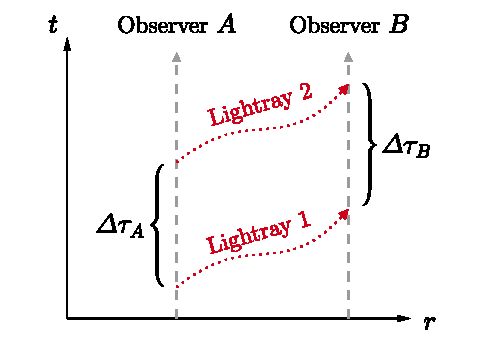
\includegraphics[width=8cm]{figures/gravredshift.pdf}
\caption{Illustration for the setting to derive the gravitational redshift.}
\label{fig:gravredshift}
\end{figure} It is not trivial to separate true gravitational shift in frequency of light from dopplerlike signals; this is only possible, if one assumes, that the two observers $A$ and $B$ are at rest radially to each other in a spherically symmetric gravitational potential. This means that the metric $g_{\alpha\beta} = g_{\alpha\beta}(t,r,\theta,\varphi)$ depends only on the radial coordinate $r$, since spherical symmetry is assumed; that is, $g_{\alpha\beta}(t,r,\theta,\varphi)=g_{\alpha\beta}(r)$. The line element associated to this metric is therefore of the form \begin{equation}
\mathrm{d}s^2(t,r,\theta,\varphi) = g_{00}(r)\,\mathrm{d}t^2 + g_{rr}(r)\,\mathrm{d}r^2 + r^2\,\mathrm{d}\theta^2 + r^2\sin^2(\theta)\,\mathrm{d}\varphi^2.
\end{equation}

Consider now observer $A$ sending out light of frequency $\nu_A$ during time $\Delta \tau_A$ towards observer $B$, which receives these signals during time $\Delta \tau_B$ and hence interprets the received frequency as $\nu_B$. Since frequency and period are inverse to one another, the frequencies and proper times of both observers can be related as \begin{equation}
\frac{\nu_A}{\nu_B} = \frac{\Delta \tau_B}{\Delta \tau_A}.
\end{equation}

A lightlike trajectory is defined, such that $\mathrm{d}s^2 = 0$, that is, a lightray only travelling in radial direction is described by \begin{equation}
\mathrm{d}s^2 = g_{00}(r)\,\mathrm{d}t^2 + g_{rr}(r)\,\mathrm{d}r^2 = 0 \quad \Leftrightarrow \quad -g_{00}(r)\,\mathrm{d}t^2 = g_{rr}(r)\,\mathrm{d}r^2, 
\end{equation} which is equivalent to stating $\frac{\mathrm{d}t}{\mathrm{d}r} = \pm \left(\frac{g_{rr}(r)}{-g_{00}(r)}\right)^{1/2}$. Integration of this equation with respect to radial distance $r$ from $r_A$ to $r_B$ yields the coordinate time $\Delta t_{j} = \int_{r_A}^{r_B}\frac{\mathrm{d}t_j}{\mathrm{d}r}\,\mathrm{d}r$ for each lightray $j$ to travel from observer $A$ to observer $B$, so we have \begin{align}\begin{aligned}
\Delta t_j = t(B)_j-t(A)_j = \int_{r_A}^{r_B} \left(\frac{g_{rr}(r)}{-g_{00}(r)}\right)^{1/2} \,\mathrm{d}r.
\end{aligned}\end{align} This means, that for two lightrays $j \in \{1,2\}$ we have \begin{equation}
t(B)_2-t(A)_2 = t(B)_1-t(A)_1 \quad \Leftrightarrow \quad \underbrace{t(B)_2-t(B)_1}_{\doteq\,\Delta t_B} = \underbrace{t(A)_2-t(A)_1}_{\doteq\,\Delta t_A},
\end{equation} indicating, that the coordinate time intervals between two pulses are equal for both observers. However, in terms of proper time, this is not the case. Since proper time is defined as $\mathrm{d}\tau = -g_{\mu\nu}\,\mathrm{d}x^\mu\,\mathrm{d}x^\nu = -g_{\mu\nu}\frac{\mathrm{d}x^\mu}{\mathrm{d}t}\frac{\mathrm{d}x^\nu}{\mathrm{d}t}\,\mathrm{d}t^2$, it follows that an interval of proper time $\Delta \tau$ is calculated as \begin{equation}
\Delta \tau = \left(-g_{\mu\nu}\frac{\mathrm{d}x^\mu}{\mathrm{d}t}\frac{\mathrm{d}x^\nu}{\mathrm{d}t}\right)^{1/2}\Delta t
\end{equation} form an interval $\Delta t$ of coordinate time, so for the proper time intervals $\tau_{A,B}$, the relation \begin{equation}
\Delta \tau_{A,B} = \left(-g_{\mu\nu}(r_{A,B})\frac{\mathrm{d}x^\mu}{\mathrm{d}t}\frac{\mathrm{d}x^\nu}{\mathrm{d}t}\right)^{1/2}\Delta t_{A,B}
\end{equation} holds. Furthermore, since the observers $A$ and $B$ were defined to be at rest to one another, as is also evident from \cref{fig:gravredshift}, the relations $\frac{\mathrm{d}x^i}{\mathrm{d}t} = 0$ and $\frac{\mathrm{d}x^0}{\mathrm{d}t} = 1$ hold for $i \in \{1,2,3\}$. Therefore, the above equation for $\Delta \tau_{A,B}$ reduces to \begin{equation}
\Delta \tau_{A,B} = \left(-g_{00}(r_{A,B})\right)^{1/2}\Delta t_{A,B}.
\end{equation} We now calculate \begin{align}
\begin{aligned}
\frac{\Delta \tau_{B}}{\Delta \tau_{A}} = \frac{(-g_{00}(r_B))^{1/2}}{(-g_{00}(r_A))^{1/2}}  \underbrace{\frac{\Delta t_B}{\Delta t_A}}_{=\,1} = \frac{(-g_{00}(r_B))^{1/2}}{(-g_{00}(r_A))^{1/2}} = \frac{\nu_A}{\nu_B}
\end{aligned}
\end{align} This means that if the gravitational field is such that $g_{00}(r_A) \neq g_{00}(r_B)$, the frequency $\nu_B$ is not the same as $\nu_A$ and hence is shifted as \begin{equation}
\nu_B = \frac{(-g_{00}(r_A))^{1/2}}{(-g_{00}(r_B))^{1/2}}\nu_A.
\end{equation} So if $-g_{00}(r_B) > -g_{00}(r_A)$, then $\nu_B < \nu_A$ and hence a redshift happens, while if $-g_{00}(r_B) < -g_{00}(r_A)$, then $\nu_B > \nu_A$ and therefore a blueshift happens.

In the case of the Newtonian limit, we have in units of $c=1$ the identity $g_{00}(r) = -(1+2\phi(r))$ and furthermore $\phi(r) = -\frac{G_N M}{r}$. With this, the above equation is
\begin{equation}
\nu_B = \sqrt{\frac{1+2\phi(r_A)}{1+2\phi(r_B)}}\nu_A = \sqrt{\frac{1-2\frac{G_N M}{r_A}}{1-2\frac{G_N M}{r_B}}}\nu_A,
\end{equation} So one can deduce the following, remarkable results, namely
\begin{align}
r_A > r_B \quad &\Leftrightarrow \quad \nu_A < \nu_B, \\
r_A < r_B \quad &\Leftrightarrow \quad \nu_A > \nu_B.
\end{align} this is to say, that if a lightray moves upwards in a gravitational field, the light is redshifted, while if a lightray moves downwards in a gravitational field, the light is blueshifted.
}

\Que{Why is it wrong to say, that a photon looses energy due to an increase in \flqq potential energy\frqq\ travelling towards weaker gravity in a gravitational field?}
\Ans{
First of all, notice that the energy $E_\gamma$ of a photon is given by $E_\gamma = h\nu_\gamma$, where $\nu_\gamma$ is the frequency of the photon. As it was calculated in the answer to the previous question, a photon will be redshifted, if its propagation direction is against gravitational pull and blueshifted, if it travels with the gravitational pull.

Since photons are neither massive particles nor non-relativistic particles, one cannot apply classical physics to it. So the conclusion, that the photon looses energy due to a rise in potential energy, if it travels against the gravitational pull, is not quite correct. The concluded statement is however correct, but the reasoning is wrong.

It is more appropriate to say, that the energy of the photon changes, since the two observer $A$ and $B$ are at a different place in the gravitational field and therefore measure energy in a different (or perturbed) metric space, because the metric $g_{\mu\nu}(r)$ is in general different at $r_A$ than it is at $r_B$.  % pages 98 and 99
}

\Que{The Einstein equivalence principle states, that in every metric space there are locally inertial (or freely falling) coordinate systems, in which the effects of gravity are absent. What does this actually mean?}
\Ans{
Consider some metric space $x^\mu$ equipped with a metric $g_{\mu\nu}(x)$. The Einstein equivalence principle actually means, that one can always go to a coordinate system $y^\alpha$ (and transform the metric accordingly to $g_{\alpha\beta}(y)$, in which the effects of gravity are locally absent. That is to say, that the metric in these new coordinate system $y^\alpha$ fulfills the equation $g_{\alpha\beta}(y) = \eta_{\alpha\beta}$, which is just the standard Minkowski metric, together with $y^\alpha$ defining Minkowski spacetime.

In this case, the geodesic equations $\ddot{x}^\mu + \Gamma^\mu_{\nu\lambda}(x)\dot{x}^\nu\dot{x}^\lambda = 0$ reduce to the equations $\ddot{y}^\alpha = 0$ of a free particle, because in the new coordinates $y^\alpha$, the Christoffel symbols are all zero, since $\Gamma^\alpha_{\beta\gamma}(y)$ involves derivatives of the metric with respect to the coordinates $y^\alpha$, and because the metric is in this case the constant Minkowski metric. % pages 101ff, section 3.6
}

\Que{How can one show, that the Einstein equivalence principle is indeed true? How can one show this either by direct construction or a numerological argument?}
\Ans{
Consider an arbitrary metric space $x^\alpha$ with an associated metric $g_{\alpha\beta}(x)$. The Einstein equivalence principle states, that there exist locally inertial coordinate systems $\xi^a$ equipped with a metric $g_{ab}(\xi)$, such that at a point $\xi_0$ in the coordinate system $\xi^a$ the effects of gravity vanish; that is to say, that $g_{ab}(\xi_0) = \eta_{ab}$ and hence $\Gamma^a_{bc}(\xi_0) = 0$ hold.

The existence of such coordinate systems $\xi^a$ can be shown by means of direct construction. Let the point $p$ in the new coordinate system $\xi^a$ be the point $x_0^\alpha$ in the old, general coordinate system $x^\alpha$. We now do a Taylor expansion of the new coordinates around the point $p$, respectively around the point $x_0^\alpha$ (noted as $x_0$) as \begin{align}\begin{aligned}
\xi^a(x) &= \xi^a(x_0) + \frac{\partial \xi^a}{\partial x^\alpha}(x_0)(x-x_0)^\alpha + \frac{1}{2}\frac{\partial^2 \xi^a}{\partial x^\beta \partial x^\gamma}(x_0)(x-x_0)^\beta(x-x_0)^\gamma + \dots \\
&= \xi^a_0 + J^a_{\alpha}(x_0)(x-x_0)^\alpha + \frac{1}{2}J^a_{\beta\gamma}(x_0)(x-x_0)^\beta(x-x_0)^\gamma + \dots.
\end{aligned}\end{align}
Here, $\frac{\partial \xi^a}{\partial x^\alpha}(x) = J^a_{\alpha}(x)$ and $\frac{\partial^2 \xi^a}{\partial x^\beta \partial x^\gamma}(x) = J^a_{\beta\gamma}(x)$ hold.

Remarking, that the metric $g_{ab}(\xi)$ transforms as \begin{equation}
g_{\alpha\beta}(x) = g_{ab}(\xi)\frac{\partial \xi^a}{\partial x^\alpha}\frac{\partial \xi^b}{\partial x^\beta} = g_{ab}(\xi)J^a_{\alpha}(x)J^b_{\beta}(x)
\end{equation} under a coordinate transformation $\xi^a \rightarrow x^\alpha$, the condition $g_{ab}(\xi_0) = \eta_{ab}$ transforms into \begin{equation} g_{\alpha\beta}(x_0) = \eta_{ab}J^a_{\alpha}(x_0)J^b_{\beta}(x_0).
\end{equation} Note, that $\eta_{ab}$ is invariant under Lorentz transformations. Comparing this to the Taylor expansion above, one sees that the Taylor expansion around a point $x_0$ in the new coordinate system $\xi^a$ is unique up to Poincaré transformations to first order.

Now, the transformation behaviour of the Christoffel symbols under a coordinate transformation $\xi^a \rightarrow x^\alpha$ is characterized as \begin{equation}
\Gamma^\alpha_{\beta\gamma}(x) = J^\alpha_{a}(\xi)J^b_{\beta}(x)J^c_{\gamma}(x)\Gamma^a_{bc}(\xi) + J^\alpha_{a}(\xi)J^a_{\beta\gamma}(x).
\end{equation} Multiplying the above equation by the inverse Jacobi matrix $J^a_{\alpha}(x)$ one can rewrite the above equation as $J^a_{\alpha}(x)\Gamma^\alpha_{\beta\gamma}(x) = J^b_{\beta}(x)J^c_{\gamma}(x)\Gamma^a_{bc}(\xi) + J^a_{\beta\gamma}(x)$. Requiring now $\Gamma^a_{bc}(\xi_0) = 0$, the above equation reads as \begin{equation}
J^a_{\alpha}(x_0)\Gamma^\alpha_{\beta\gamma}(x_0) = \underbrace{\Gamma^a_{bc}(\xi_0)J^b_{\beta}(x_0)J^c_{\gamma}(x_0)}_{=\,0} + J^a_{\beta\gamma}(x_0).
\end{equation} Again comparing this result to the Taylor expansion around a point $x_0$ in the new coordinate system $\xi^a$ yields, that this new coordinate system exists and is unique up to Poincaré transformations. Since there are an infinite number of higher-order terms undetermined, this shows, that the constructed coordinate system is overall highly non-unique, but that these locally inertial systems indeed do exist. Remember, that the conditions hereof were, that the metric $g_{ab}(\xi)$ reduces to $\eta_{ab}$ and that for the Christoffel symbols $\Gamma^a_{bc}(\xi) = 0$ holds.
% p 102ff$
}

\Que{Why is \flqq general covariance\frqq\ relevant for describing physics in a gravitational field?}
\Ans{
First recall, what the principle of general covariance in general relativity states; it is a combination of the general principle of covariance in physics and the Einstein equivalence principle. Considering a metric space $x^\mu$ associated to an arbitrary gravitational field described by the metric $g_{\mu\nu}=g_{\mu\nu}(x)$, a physical equation satisfies the principle of general covariance if two requirements are met:
\begin{enumerate}
\item The equation must hold in the absence of gravity; that is, if a coordinate transformation $x^\mu\rightarrow y^a$ is conducted on the equation, such that the effects of gravity vanish, i.e. $g_{ab} = g_{ab}(y) = \eta_{ab}$ and hence $\Gamma^a_{bc} = \Gamma^a_{bc}(y) = 0$, the physical equation must still hold.
\item The equation must be generally covariant, which is to say, that it preserves its form under a general coordinate transformation $x^\mu \rightarrow y^a$.
\end{enumerate} 

With this in mind it becomes evident, why \flqq general covariance\frqq\ is relevant for describing physics in a gravitational field. Namely, because of the Einstein equivalence principle, one can always choose a coordinate system, such that the effects of gravity vanish. What one further wants is, that under these coordinate transformations the physical equations preserve their form, therefore general covariance is needed.% See p. 110ff
}

\Que{Which two conditions must be fulfilled for an equation, such that it holds in an arbitrary gravitational field by virtue of the Einstein equivalence principle?}
\Ans{
In order for an equation to hold in an arbitrary gravitational field, it must fulfill the following two conditions, usually referred to as the principle of general covariance:
\begin{enumerate}
\item The equation must hold in the absence of gravity.
\item The equation must preserve its form under general coordinate transformations.
\end{enumerate} % page 111ff
}

\Que{How does algorithm of minimal coupling work to produce equations satisfying general covariance and special relativity?}
\Ans{
Recall, that a generally covariant equation will be valid in an arbitrary gravitational field, provided that it is valid in Minkowski space. Therefore, we can develop a strategy, by which we can construct generally covariant equations - this strategy/principle is called minimal coupling and it works as follows:
\begin{enumerate}
\item Start with an equation in inertial coordinates $\xi^a$ satisfying special relativity.
\item Replace the inertial coordinates $\xi^a$ by arbitrary coordinates $x^\mu$, namely \begin{equation}\xi^a \mapsto x^\mu. 
\end{equation}
\item Substitute all appearances of the Minkowski metric $\eta_{ab}$ with the metric $g_{\mu\nu}(x)$ describing the gravitational field, i.e. \begin{equation} \eta_{ab} \mapsto g_{\mu\nu}(x). \end{equation}
\item Promote Lorentz tensors $T^{a\dots}_{b\dots}$ to tensors $T^{\mu\dots}_{\nu\dots}$ under general coordinate transformations, i.e. \begin{equation}
T^{a\dots}_{b\dots}(\xi) \mapsto T^{\mu\dots}_{\nu\dots}(x).
\end{equation}
\item Substitute all partial derivatives $\partial_a = \partial_{\xi_a}$ with the covariant derivative $\nabla_\mu$, namely \begin{equation}
\partial_a \mapsto \nabla_\mu = \partial_\mu + \Gamma^\nu_{\mu\lambda}.
\end{equation}
\item Replace potentially present derivatives $\frac{\mathrm{d}}{\mathrm{d}\tau}$ with the appropriate generally covariant expression, namely \begin{equation}
\frac{\mathrm{d}}{\mathrm{d}\tau} = \frac{\mathrm{d}\xi^a}{\mathrm{d}\tau}\frac{\partial}{\partial \xi^a} = \dot{\xi}^a \partial_a \mapsto \dot{x}^\mu \nabla_\mu.
\end{equation}
\item Substitute all integrals $\int_{\mathbb{R}^4} \mathrm{d}^4\xi$ with the covariant integrals, namely \begin{equation}
\int_{\mathbb{R}^4} \mathrm{d}^4\xi \mapsto \int_{\mathbb{R}^4} \sqrt{g}\,\mathrm{d}^4 x,
\end{equation} where $g \doteq |\det(g_{\mu\nu}(x))|$.
\end{enumerate}

Now, by construction the resulting equation is both generally covariant and furthermore holds in the absence of gravity.% p. 175ff
}

\Que{Give an example of how the minimal coupling algorithm works!}
\Ans{
Consider the equation of motion for a free particle with mass $m$, namely \begin{equation}
ma^a = m\frac{\mathrm{d}u^a}{\mathrm{d}\tau} = m \frac{\mathrm{d}}{\mathrm{d}\tau}\left(\frac{\mathrm{d}\xi^a}{\mathrm{d}\tau}\right)= 0,
\end{equation} where $u^a$ is the four velocity. First, we substitute $\nicefrac{\mathrm{d}\xi^a}{\mathrm{d}\tau} \mapsto \nicefrac{\mathrm{d}x^\mu}{\mathrm{d}\tau} = u^\mu = \dot{x}^\mu$. Next, we substitute $\nicefrac{\mathrm{d}}{\mathrm{d}\tau} \mapsto \dot{x}^\nu \nabla_\nu = u^\nu\nabla_\nu$ and get \begin{align}\begin{aligned}
\dot{x}^\nu \nabla_\nu \dot{x}^\mu &= \dot{x}^\nu\left(\partial_\nu \dot{x}^\mu + \Gamma^\mu_{\nu\lambda}\dot{x}^\lambda\right) = \dot{x}^\nu \frac{\mathrm{d}^2 x^\mu}{\mathrm{d}\tau}\underbrace{\frac{\mathrm{d}\tau}{\mathrm{d}x^\nu}}_{=(\dot{x}^\nu)^{-1}} + \Gamma^\mu_{\nu\lambda} \dot{x}^\nu\dot{x}^\lambda = \ddot{x}^\mu + \Gamma^\mu_{\nu\lambda} \dot{x}^\nu\dot{x}^\lambda = 0,
\end{aligned}\end{align} thus the generally covariant geodesic equation results, which simplifies again to the free motion equation in the case where one has $g_{\mu\nu} = \eta_{\mu\nu}$.
}

\section{Tensor algebra}
\Que{How can the basic objects of tensor algebra be defined and what properties do they have?}
\Ans{
In order to construct a physical theory with generally covariant equations, objects are needed that transform in a simple way under general coordinate transformations \begin{equation}
x^\alpha \rightarrow y^\mu(x) = \bar{x}^\mu(x).
\end{equation} Such objects are tensors; scalars and vectors are just examples of tensors. Tensors transform multi-linearly with the Jacobi matrices of the coordinate transformation $x^\alpha \rightarrow y^\mu(x) = \bar{x}^\mu(x)$, namely \begin{equation}
J^\mu_{\alpha} = \frac{\partial \bar{x}^\mu}{\partial x^\alpha} = \frac{\partial y^\mu}{\partial x^\alpha}, \quad J^{\alpha}_{\mu} = \frac{\partial x^\alpha}{\partial \bar{x}^\mu} = \frac{\partial x^\alpha}{\partial y^\mu},
\end{equation} which satisfy the equations \begin{equation}
J_{\mu}^{\alpha}J^\mu_{\beta} = \delta^\alpha_{\beta}, \quad J^\mu_\alpha J^\alpha_\nu = \delta^\mu_\nu.
\end{equation}

There are six main types of tensors to distinguish; scalars, vectors, covectors, covariant 2-tensors, contravariant 2-tensors and general pq-tensors, all of which will now briefly be discussed. Let for the following considerations $x^\alpha$ be coordinates of a metric space and $x^\alpha \rightarrow \bar{x}^\mu(x)$ a general coordinate transformation to new coordinates.

\paragraph{Scalars} An object $f(x)$ that transforms as \begin{equation}
\bar{f}(\bar{x}(x)) = f(x),
\end{equation} under a general coordinate transformation is called a scalar. 

\paragraph{Vectors} An object $V^\alpha(x)$ that transforms as \begin{equation}
\bar{V}^\mu(\bar{x}(x)) = J^\mu_\alpha(x)V^\alpha(x)
\end{equation} under a general coordinate transformation is called a vector.

\paragraph{Covector} An object $U_\alpha(x)$ that transforms inversely to a vector, namely as \begin{equation}
\bar{U}_\mu(\bar{x}(x)) = J^\alpha_\mu(\bar{x}(x))U_\alpha(x)
\end{equation} under a general coordinate transformation is called a covector. A covector can also be considered as a contravariant vector.

\paragraph{Covariant 2-tensors} An object $A_{\alpha \beta}(x)$ that transforms like the product of two covectors, namely \begin{equation}
\bar{A}_{\mu\nu}(\bar{x}(x)) \overset{\text{Not.}}{=} A_{\mu\nu}(\bar{x}(x)) = J^\alpha_\mu(\bar{x}(x))J^\beta_\nu(\bar{x}(x))A_{\alpha\beta}(x)
\end{equation} under a general coordinate transformation is called a covariant 2-tensor, or more precisely a (0,2)-tensor.

\paragraph{Contravariant 2-tensors} An object $B^{\alpha \beta}(x)$ that transforms like the product of two vectors, namely \begin{equation}
\bar{B}^{\mu\nu}(\bar{x}(x)) \overset{\text{Not.}}{=} B^{\mu\nu}(\bar{x}(x)) = J^\mu_\alpha(x)J^\nu_\beta(x)B_{\alpha\beta}(x)
\end{equation} under a general coordinate transformation is called a contravariant 2-tensor, or more precisely a (2,0)-tensor.

\paragraph{pq-tensors} An object $T^{\alpha_1\dots\alpha_p}_{\beta_1\dots\beta_q}(x)$ that transforms like the product of $p$ vectors and $q$ covectors, namely \begin{equation}
T^{\mu_1\dots\mu_p}_{\nu_1\dots\nu_q} = J^{\mu_1}_{\alpha_1}\dots J^{\mu_p}_{\alpha_p} J^{\beta_1}_{\nu_1}\dots J^{\beta_q}_{\nu_q}T^{\alpha_1\dots \alpha_p}_{\beta_1\dots\beta_q}
\end{equation} under a general coordinate transformation is called a general pq-tensor.
% page 110ff
}

\section{Tensor analysis}
\Que{How is the formula $\delta g = g g^{\nu\mu}\delta g_{\mu\nu}$ for a variation of the determinant $g \doteq |\det(g_{\mu\nu})|$ of a metric proven?}
\Ans{
Notice first, that the determinant $g$ can be calculated by the cofactor expansion formula for arbitrary index $\mu$ as \begin{equation}
g = \sum_{\nu} (-1)^{\mu+\nu}g_{\mu\nu}\det(m_{\mu\nu}),
\end{equation} with $m_{\mu\nu}$ being the matrix obtained from $g_{\mu\nu}$ by removing the $\mu$'th row and $\nu$'th column. From this, \begin{equation}
\sum_{\nu}(-1)^{\mu+\nu}g_{\lambda\nu}\det(m_{\mu\nu}) = 0, \quad \mu \neq \lambda,
\end{equation} because this means $g_{\mu\nu} = g_{\lambda\nu}$ (two rows are equal to one another), hence the determinant of such a matrix must be zero, because two rows are linearly dependent, thus the rank of the matrix cannot be full. Combined, the above two formulae yield \begin{equation}
g \delta_{\lambda\mu} = \sum_{\nu}(-1)^{\mu+\nu} g_{\lambda\nu}\det(m_{\mu\nu}).
\end{equation} Multiplying it with the inverse metric $g^{\nu\mu}$ yields \begin{align}
\begin{aligned}
g^{\nu\mu}\sum_{\nu}(-1)^{\mu+\nu}g_{\lambda\nu}\det(m_{\mu\nu}) = \delta_{\lambda\mu} g g^{\nu\mu} \quad &\Leftrightarrow \quad (-1)^{\mu+\nu}\delta_{\lambda\mu}\det(m_{\mu\nu}) = \delta_{\lambda\mu} g g^{\nu\mu} \\
&\Leftrightarrow \quad g^{\nu\mu} = (-1)^{\mu\nu}\frac{\det(m_{\mu\nu})}{g}.
\end{aligned}
\end{align} This is a valid formula to calculate any inverse matrix. Now, we take this formula and multiply times $g$ and times $g_{\mu\lambda}$, thus obtaining \begin{align}
\begin{aligned}
g g^{\nu\mu}g_{\mu\lambda} = (-1)^{\mu+\nu}\det(m_{\mu\nu})g_{\mu\lambda} \quad \Leftrightarrow \quad g &= (-1)^{\mu+\nu}\det(m_{\mu\nu})g_{\mu\lambda}\delta_{\nu\lambda} \\ &= (-1)^{\mu+\nu}\det(m_{\mu\nu})g_{\mu\nu} = g(g_{\mu\nu}).
\end{aligned}
\end{align} Now, assuming $g(g_{\mu\nu})$ is a smooth function of $g_{\mu\nu}$, we can differentiate and obtain \begin{equation}
\frac{\partial g(g_{\mu\nu})}{\partial g_{\mu\nu}} = (-1)^{\mu+\nu}\det(m_{\mu\nu}) = g g^{\nu\mu}.
\end{equation} Finally, we can examine the structure of the variation of the determinant of a metric, namely $g \rightarrow g  + \delta g$. The term $\delta g$ is given by \begin{equation}
\delta g = \frac{\partial g}{\partial g_{\mu\nu}}\delta g_{\mu\nu} = g g^{\nu\mu} \delta g_{\mu\nu},
\end{equation} thus, the formula is proven. 

Note, that the variation of the square root of the determinant is given as \begin{equation}
\delta \sqrt{g} = \frac{1}{2\sqrt{g}}\delta g = \frac{1}{2}\frac{g}{\sqrt{g}} g^{\nu\mu}\delta g_{\mu\nu} = \frac{1}{2}\sqrt{g} g^{\nu\mu}\delta g_{\mu\nu} = -\frac{1}{2}\sqrt{g}g_{\nu\mu}\delta g^{\mu\nu}.
\end{equation}
}

\Que{How is the identity $\Gamma^\mu_{\mu\lambda} = \frac{1}{\sqrt{g}}\partial_\lambda \sqrt{g}$ connecting the Christoffel symbols with the determinant $g \doteq |\det(g_{\mu\nu})|$ of a metric proven?}
\Ans{
First of all, note the formula $\delta g = g g^{\nu\mu}\delta g_{\mu\nu} = gg^{\mu\nu}\delta g_{\mu\nu}$ form symmetric metrics and $g \doteq |\det(g_{\mu\nu})|$. Additionally, we have the formula $\delta \sqrt{g} = \frac{1}{2}\sqrt{g}g^{\mu\nu}\delta g_{\mu\nu}$.

Now, we calculate the \flqq variation\frqq\ of $g$ with respect to the space $x^\lambda$, namely \begin{equation}
\partial_\lambda g = \frac{\partial}{\partial x^\lambda} g = \frac{\partial g}{\partial g_{\mu\nu}}\frac{\partial g_{\mu\nu}}{\partial x^\lambda} = g g^{\mu\nu} g_{\mu\nu,\lambda} = g g^{\mu\nu}\partial_\lambda g_{\mu\nu}.
\end{equation} Also, we can calculate the \flqq variation\frqq\ of $\sqrt{g}$ with respect to $x^\lambda$, hence we get \begin{equation}
\partial_\lambda \sqrt{g} = \frac{\partial}{\partial x^\lambda}\sqrt{g} = \frac{\partial \sqrt{g}}{\partial g}\frac{\partial g}{\partial g_{\mu\nu}}\frac{\partial g_{\mu\nu}}{\partial x^\lambda} = \frac{1}{2\sqrt{g}}g g^{\mu\nu}\partial_\lambda g_{\mu\nu} = \frac{1}{2}\sqrt{g} g^{\mu\nu}\partial_\lambda g_{\mu\nu}.
\end{equation} Now, the Christoffel symbols are defined as \begin{equation}
\Gamma^\mu_{\nu\lambda} = g^{\mu\rho}\Gamma_{\rho\nu\lambda} = g^{\mu\rho}\frac{1}{2}(g_{\rho\nu,\lambda}+ g_{\rho\lambda,\nu}-g_{\nu\lambda,\rho}). 
\end{equation} Calculating $\Gamma^{\mu}_{\mu\lambda}$ yields \begin{align}
\begin{aligned}
\Gamma^{\mu}_{\mu\lambda} &= g^{\mu\rho}\Gamma_{\rho\mu\lambda} = \frac{1}{2}g^{\mu\rho}(g_{\rho\mu,\lambda}+g_{\rho\lambda,\mu}-g_{\mu\lambda,\rho}) = \frac{1}{2}\left(g^{\mu\rho}g_{\rho\mu,\lambda}+ \underbrace{g^{\mu\rho}g_{\rho\lambda,\mu}-g^{\mu\rho}g_{\mu\lambda,\rho}}_{=\,0}\right) \\
&= \frac{1}{2}g^{\mu\rho}g_{\mu\rho,\lambda} = \frac{1}{2}g^{\mu\nu}\partial_\lambda g_{\mu\nu}.
\end{aligned}
\end{align} Comparing this to the above results yields the equalities \begin{equation}
\Gamma^{\mu}_{\mu\lambda} = \frac{1}{2}g^{\mu\nu} \partial_\lambda g_{\mu\nu} = \frac{1}{\sqrt{g}}\partial_\lambda \sqrt{g} = \frac{1}{2}g^{-1}\partial_\lambda g.
\end{equation}
}

\Que{Let the covariant Laplacian be defined as $\Box \doteq g^{\alpha\beta}\nabla_\alpha \nabla_\beta$. How can the Laplacian be calculated in an easy way, relying on the formula for the variation of a determinant?}
\Ans{
We first show, that the covariant divergence $\nabla_\mu J^\mu$ of a vector $J^\mu$ is calculated as $\nabla_\mu J^\mu = \frac{1}{\sqrt{g}}\partial_\mu (\sqrt{g}J^\mu)$. To this end, we use the identity $\Gamma^\mu_{\mu\lambda} = \frac{1}{\sqrt{g}}\partial_\lambda \sqrt{g}$ and calculate \begin{equation}
\nabla_\mu J^\mu = \partial_\mu J^\mu + \Gamma^{\mu}_{\mu\lambda}J^\lambda = \partial_\mu J^\mu + \frac{1}{\sqrt{g}}\left(\partial_\lambda \sqrt{g}\right) J^\lambda.
\end{equation} Furthermore, the derivative \begin{equation}
\partial_\mu (\sqrt{g}J^\mu) = J^\mu \partial_\mu \sqrt{g} + \sqrt{g}\partial_\mu J^\mu = \sqrt{g}\left(\frac{1}{\sqrt{g}}J^\lambda(\partial_\lambda \sqrt{g})+\partial_\mu J^\mu\right) = \sqrt{g}\nabla_\mu J^\mu
\end{equation} is obtained, wherefrom we can finally derive \begin{equation}
\nabla_\mu J^\mu = \frac{1}{\sqrt{g}}\partial_\mu(\sqrt{g}J^\mu).
\end{equation} Consider now a scalar $f$; for scalars we have $\nabla_\mu f = \partial_\mu f$. Considering $\nabla_\mu g^{\mu\nu} = 0$, we can write \begin{equation}
\Box f = g^{\mu\nu}\nabla_\mu\nabla_\nu f = \nabla_\mu(g^{\mu\nu}\nabla_\nu f) = \frac{1}{\sqrt{g}}\partial_\mu(\sqrt{g}g^{\mu\nu}\nabla_\nu f) = \frac{1}{\sqrt{g}}\partial_\mu(\sqrt{g}g^{\mu\nu}\partial_\nu f).
\end{equation} Hence the covariant Laplacian $\Delta \rightarrow \Box$ in some space $x^\mu$ described by the metric $g_{\mu\nu}(x)$ can be written as \begin{equation}
\Box = \frac{1}{\sqrt{g}}\partial_\mu(\sqrt{g}g^{\mu\nu}\partial_\nu).
\end{equation} This is a useful formula to e.g. calculate the Laplacian of euclidean space in polar coordinates, which would otherwise be a very tedious task without this formula.
}

\Que{What does it mean, when the curvature tensor of some metric space in arbitrary coordinates is zero?}
\Ans{
If the curvature of an arbitrary metric space is zero, it means that there is a coordinate transformation from the coordinate of the metric space to Minkowski space. % If curvature of some space in arbitrary coordinates is zero, then there is a coordinate transformation to Minkowski space
}

\Que{How does generally covariant integration work and what are the properties of the volume elements of metric spaces?}
\Ans{
Consider a metric space $x^\mu$ and a general coordinate transformation $x^\mu \rightarrow \bar{x}^\alpha(x)$. Let furthermore $f(x)$ be a scalar. Generally, the integral over spacetime of the scalar in the new coordinates will not be equal to the same integral in the old coordinates, i.e. \begin{equation}
\int_{\mathbb{R}^4} f(x)\,\mathrm{d}^4x \neq \int_{\mathbb{R}^4} \bar{f}(\bar{x})\,\mathrm{d}^4\bar{x},
\end{equation} hence the integral of a scalar $f(x)$ over spacetime cannot be considered as being generally covariant, i.e. preserving its form under general coordinate transformations.

But the integral of any scalar can be made generally covariant by means of introducing a so-called tensor density $\rho(x)$ constructed from the metric $g_{\mu\nu}(x)$ of spacetime. Note, that the measure $\mathrm{d}^4x$ transforms as \begin{equation}
\mathrm{d}^4\bar{x} = \left|\det\left(\frac{\partial \bar{x}}{\partial x}\right)\right|\,\mathrm{d}^4 x, \qquad \bar{x} = \bar{x}^\alpha, \ x = x^\mu
\end{equation} under a general coordinate transformation $x^\mu \rightarrow \bar{x}^\alpha(x)$. If one finds a tensor density $\rho(x)$ which transforms as \begin{equation}
\bar{\rho}(\bar{x}) = \left|\det\left(\frac{\partial \bar{x}}{\partial x}\right)\right|^{-1}\,\rho(x)
\end{equation} under the same general coordinate transformation, one can write down a generally covariant integral of a scalar $f(x)$, namely \begin{equation}
\int_{\mathbb{R}^4} \bar{\rho}(\bar{x})\bar{f}(\bar{x})\,\mathrm{d}^4\bar{x} = \int_{\mathbb{R}^4}\rho(x)f(x)\,\mathrm{d}^4x.
\end{equation}

Recall, that the metric $g_{\mu\nu}(x)$ transforms as \begin{equation}
\bar{g}_{\alpha\beta}(\bar{x}) = \frac{\partial x^\mu}{\partial \bar{x}^\alpha}(\bar{x})\frac{\partial x^\nu}{\partial \bar{x}^\beta}(\bar{x})g_{\mu\nu}(x)
\end{equation} under the mentioned coordinate transformation. Due to the multiplicative property of the determinant, one can write \begin{align}
\begin{aligned}
\det\left(\bar{g}_{\alpha\beta}(\bar{x})\right) = \det\left(\frac{\partial x^\mu}{\partial \bar{x}^\alpha}(\bar{x})\right)\det\left(\frac{\partial x^\nu}{\partial \bar{x}^\beta}(\bar{x})\right)\det\left(g_{\mu\nu}(x)\right)
\end{aligned}
\end{align} and hence
\begin{align}
\begin{aligned}
\left|\det\left(\bar{g}_{\alpha\beta}(\bar{x})\right)\right| = \left|\det\left(\frac{\partial x}{\partial \bar{x}}\right)\right|^2\left|\det\left(g_{\mu\nu}(x)\right)\right| = \left|\det\left(\frac{\partial \bar{x}}{\partial x}\right)\right|^2\left|\det\left(g_{\mu\nu}(x)\right)\right|.
\end{aligned}
\end{align} Adopting the notation $\left|\det\left(\bar{g}_{\alpha\beta}(\bar{x})\right)\right| \doteq \bar{g}$ and $\left|\det\left(g_{\mu\nu}(x)\right)\right| \doteq g$, we can hence write \begin{equation}
\sqrt{\bar{g}} = \sqrt{\bar{g}(\bar{x})} = \left|\det\left(\frac{\partial \bar{x}}{\partial x}\right)\right|^{-1}\sqrt{g(x)}.
\end{equation} Comparing this to the above requirement to a tensor density $\rho(x)$ such that the integral over spacetime of a scalar $f(x)$ ins generally covariant, one identifies $\rho(x) = \sqrt{g(x)}$ and $\bar{\rho}(\bar{x}) = \sqrt{\bar{g}(\bar{x})}$ and can therefore write down a generally covariant integral \begin{equation}
\int_{\mathbb{R}^4} \sqrt{\bar{g}(\bar{x})}\bar{f}(\bar{x})\,\mathrm{d}^4\bar{x} = \int_{\mathbb{R}^4} \sqrt{g(x)}f(x)\,\mathrm{d}^4x.
\end{equation}% page 123ff

With this rule, one can easily perform a transformation of the volume element $\mathrm{d}^3x$ from cartesian coordinates with $\sqrt{g} = 1$ to some other coordinates with known tensor density $\sqrt{\bar{g}}$, because in this case the volume element transforms as \begin{equation}
\mathrm{d}^3x = \sqrt{\bar{g}}\,\mathrm{d}^3\bar{x}.
\end{equation}
}

\Que{How does generally covariant differentiation work?}
\Ans{
Consider a metric space $x^\mu$ equipped with a metric $g_{\mu\nu}(x)$. What one would like to have is, that the derivatives of vector (fields) transform as tensors under general coordinate transformations, i.e. with the Jacobi matrices of the transformation rule. Given a vector $V^\mu(x)$ and a coordinate transformation $x^\mu \rightarrow y^\alpha$, the partial derivative $\partial_\beta V^\alpha$ transforms as \begin{equation}
\partial_\beta V^\alpha = J^\nu_\beta J^\alpha_\mu \partial_\nu V^\mu + J^\nu_\beta J^\alpha_{\mu\nu} V^\mu,
\end{equation} taking into account the transformation behaviour of the partial derivative $\partial_\mu$ and the vector $V^\mu$ under the specified transformation, which is accounted for by \begin{equation}
\partial_\alpha = \frac{\partial}{\partial y^\alpha} = \frac{\partial x^\mu}{\partial y^\alpha}\frac{\partial}{\partial x^\mu} = J^\mu_\alpha \partial_\mu, \qquad V^\alpha = J^\alpha_\mu V^\mu.
\end{equation} This shows, that the partial derivative of a vector (field) is not a tensor. In order to construct a means of differentiating in a covariant way, one can define the so-called covariant derivative $\nabla_\nu V^\mu$, which is generally covariant and is defined as \begin{equation}
\nabla_\nu V^\mu = \partial_\nu V^\mu + \Gamma^\mu_{\nu\lambda}V^\lambda.
\end{equation} It can be shown, that this object indeed transforms as a (1,1)-tensor under coordinate transformations $x^\mu\rightarrow y^\alpha(x)$. % page 146ff
}

\Que{What is the Leibniz rule for differentiating a product of tensors?}
\Ans{
The Leibniz rule for differentiating a product of tensor is just an application of the product rule for differentiation. It is given as \begin{equation}
\nabla_\mu (A^{\mu_1\dots\mu_p}_{\nu_1\dots\nu_q}B^{\rho_1\dots\rho_r}_{\lambda_1\dots\lambda_s}) = B^{\rho_1\dots\rho_r}_{\lambda_1\dots\lambda_s} \nabla_\mu A^{\mu_1\dots\mu_p}_{\nu_1\dots\nu_q} + A^{\mu_1\dots\mu_p}_{\nu_1\dots\nu_q}\nabla_\mu B^{\rho_1\dots\rho_r}_{\lambda_1\dots\lambda_s}.
\end{equation} % p. 150ff
}

\Que{How does covariant differentiation of a covector work?}
\Ans{
The covariant differentiation of a covector $V_\mu$ is given by \begin{equation}
\nabla_\nu V_\mu = \partial_\nu V_\mu - \Gamma^{\lambda}_{\nu \mu}V_\lambda.
\end{equation}
}

\Que{How is the covariant derivative of a general $(p,q)$-tensor defined?}
\Ans{
Using the formulae for the covariant differentiation of a vector $V^\mu$ and a covector $V_\mu$ \begin{equation}
\nabla_\mu V^\nu = \partial_\mu V^\nu + \Gamma^\nu_{\mu\lambda} V^\lambda \quad , \quad \nabla_\mu V_\nu = \partial_\mu V_\nu - \Gamma^{\lambda}_{\mu\nu} V_\lambda ,
\end{equation} one can derive the general formula \begin{align}\begin{aligned}
\nabla_\mu T^{\nu_1\dots\nu_p}_{\rho_1\dots\rho_q} &= \partial_\mu T^{\nu_1\dots\nu_p}_{\rho_1\dots\rho_q} \\
&+ \Gamma^{\nu_1}_{\mu\lambda}T^{\lambda\nu_2\dots\nu_p}_{\rho_1\dots\rho_q} + \dots + \Gamma^{\nu_p}_{\mu\lambda}T^{\nu_1\dots\nu_{p-1}\lambda}_{\rho_1\dots\rho_q} \\ &- \Gamma^{\lambda}_{\mu\rho_1}T^{\nu_1\dots\nu_p}_{\lambda\rho_2\dots\rho_q} - \dots - \Gamma^{\lambda}_{\mu\rho_q}T^{\nu_1\dots\nu_p}_{\rho_1\dots\rho_{q-1}\lambda}.
\end{aligned}\end{align} For example, the covariant derivative of a $(1,1)$-tensor $T^{\mu}_{\nu}$ is given as \begin{equation}
\nabla_\lambda T^{\mu}_\nu = \partial_\lambda T^\mu_\nu + \Gamma^\mu_{\lambda \gamma}T^\gamma_\nu - \Gamma^{\gamma}_{\lambda \nu}T^\mu_\lambda.
\end{equation}
}

\Que{Why does the covariant curl of a covector reduce to just the normal curl?}
\Ans{
The normal curl of a covector $U_\mu$ is given by $\partial_\mu U_\nu - \partial_\nu U_\mu$. The covariant curl is given by \begin{align}
\begin{aligned}
\nabla_\mu U_\nu - \nabla_\nu U_\mu = \partial_\mu U_\nu - \Gamma_{\mu\nu}^\lambda U_\lambda - \partial_\nu U_\mu + \Gamma_{\nu\mu}^\lambda U_\lambda = \partial_\mu U_\nu - \partial_\nu U_\mu,
\end{aligned}
\end{align} because $\Gamma_{\mu\nu}^\lambda = \Gamma_{\nu\mu}^\lambda$.
}

\Que{How is the covariant divergence defined, and how can the divergence in spherical coordinates easily be derived?}
\Ans{
The covariant divergence of a vector $V^\mu$ is defined as $\nabla_\mu V^\mu$ and it is by previous calculations given as \begin{equation}
\nabla_\mu V^\mu = \partial_\mu V^\mu + \Gamma^{\mu}_{\mu\lambda}V^\lambda = \frac{1}{\sqrt{g}}\partial_\mu (\sqrt{g}V^\mu),
\end{equation} where $g \doteq |\det(g_{\mu\nu})|$ is the determinant of the metric $g_{\mu\nu}$.  %p. 156ff
}

\Que{How is the covariant derivative along a curve defined?}
\Ans{
Consider some space $x^\mu$; and a curve parametrized by a parameter $\tau$, e.g. proper time, such that $x^\mu = x^\mu(\tau)$. Differentiation along a curve is just the projection of the derivative $\nicefrac{\partial}{\partial x^\mu}$ projected onto the tangent vector field $\dot{x}^\mu$ along the curve at a point $x^\mu(\tau)$, such that one has \begin{equation}
\dot{x}^\mu\partial_\mu = \left(\frac{\mathrm{d}x^\mu(\tau)}{\mathrm{d}\tau}\right)\frac{\partial}{\partial x^\mu} = \frac{\mathrm{d}}{\mathrm{d}\tau}
\end{equation} for the derivative along a curve. Covariantising this with the minimal coupling procedure $\partial_\mu \rightarrow \nabla_\mu$ yields \begin{equation}
\dot{x}^\mu \nabla_\mu \doteq D_\tau
\end{equation} for the covariant derivative along a curve.% p. 162ff
}

%\Que{How can the identity $\det(\matr{M}) = e^{\mathrm{tr}(\ln(\matr{M}))}$ be proven for $\matr{M}$ a diagonalizable matrix?}
%\Ans{
%Let this assertion first be stated properly:
%\begin{ass}
%Let $\matr{M}$ be a diagonalizable matrix. For such a matrix, the identity $\det(\matr{M}) = e^{\mathrm{tr}(\ln(\matr{M}))}$ holds.
%\end{ass} 
%\begin{proof}
%Since $\matr{M}$ is diagonalizable, it can be written as $\matr{M} = \matr{P}\matr{D}\matr{P}^{-1}$, where $\matr{D}$ is the diagonal matrix of eigenvalues on the diagonal line and $\matr{P}$ is a matrix of eigenvectors. Note, that the trace of a product of matrices is the same as the product of their traces; this means we have \begin{equation}
%\mathrm{tr}(\ln(\matr{M})) = \mathrm{tr}(\ln(\matr{P}))\mathrm{tr}(\ln(\matr{D}))\mathrm{tr}(\ln(\matr{P}^{-1})) = \mathrm{tr}(\ln(\matr{D}))
%\end{equation}
%\end{proof}
%}

\section{Schwarzschild metric}
\Que{What does stationarity mean in the context of metrics? What does static mean?}
\Ans{
Consider some metric space $x^\mu$ and an associated metric $g_{\mu\nu}(x)$. A stationary metric $g_{\mu\nu}$ is a metric without explicit time dependence, i.e. \begin{equation}
\frac{\partial}{\partial t}g_{\mu\nu}(x) = 0.
\end{equation} That is to say, a stationary metric is invariant under time translations $t\rightarrow t+ c$, where $c$ is an arbitrary constant.

A static metric $g_{\mu\nu}(x)$ however is a metric, which is in addition to stationarity also invariant under time reflections $t\rightarrow c-t$.% 
}

\Que{What is a static spherically symmetric metric? What does it describe?}
\Ans{
The most general form of a static spherically symmetric metric is accounted for by the line element \begin{equation}
\mathrm{d}s^2 = -A(r)\,\mathrm{d}t^2 + B(r)\,\mathrm{d}r^2 + r^2\,\mathrm{d}\theta^2 + r^2\sin^2(\theta)\,\mathrm{d}\varphi^2.
\end{equation} Therefore, the general form of a static spherically symmetric metric $g_{\mu\nu}(x)$ in coordinates $x^\mu = (ct, r, \theta, \varphi)$ (or sometimes with units $c=1$) is given as \begin{equation}
g_{\mu\nu}(x) = \begin{pmatrix} 
-A(r) & 0 & 0 & 0 \\
0 & B(r) & 0 & 0 \\
0 & 0 & r^2 & 0 \\
0 & 0 & 0 & r^2\sin^2(\theta)
\end{pmatrix},
\end{equation} where $c$ can be absorbed in $A(r)$. A static spherically symmetric metric describes very well the exterior of a normal star; neither the gravitational field of a star does not change significantly with time, nor are there any significant deviations of spherical symmetry to be expected.  % see p. 506ff
}

\Que{What are the Schwarzschild coordinates?}
\Ans{
The standard Schwarzschild coordinates are $x^\mu = (t,r,\theta,\varphi)$, which describe a static spherically symmetric geometry. % see p.514ff
}

\Que{What is the Schwarzschild metric, what does it describe and what are its key properties?}
\Ans{
The line element in the Schwarzschild metric is given in full by \begin{equation}
\mathrm{d}s^2 = -\left(1-\frac{2MG_N}{c^2 r}\right)c^2\,\mathrm{d}t^2 + \left(1-\frac{2MG_N}{c^2r}\right)^{-1}\,\mathrm{d}r^2 + r^2\,\mathrm{d}\theta^2 + r^2\sin^2(\theta)\,\mathrm{d}\varphi^2,
\end{equation} where the metric is given by \begin{equation}
g_{\mu\nu}(x) = \begin{pmatrix}
-\left(1-\frac{2MG_N}{c^2r}\right) & 0 & 0 & 0 \\
0 & \left(1-\frac{2MG_N}{c^2 r}\right)^{-1} & 0 & 0 \\
0 & 0 & r^2 & 0 \\
0 & 0 & 0 & r^2\sin^2(\theta)
\end{pmatrix}
\end{equation} with the Schwarzschild coordinates $x^\mu = (ct, r, \theta, \varphi)$. Defining the constant $m \doteq MG_N/c^2$, the function $f(r) = 1-2m/r$ and setting $c=1$, the line element in the Schwarzschild metric reduces to \begin{equation}
\mathrm{d}s^2 = -f(r)\,\mathrm{d}t^2 + f(r)^{-1}\,\mathrm{d}r^2 + r^2\,\mathrm{d}\theta^2 + r^2\sin^2(\theta)\,\mathrm{d}\varphi^2
\end{equation} with the metric \begin{equation}
g_{\mu\nu}(x) = \begin{pmatrix}
-f(r) & 0 & 0 & 0 \\
0 & f(r)^{-1} & 0 & 0 \\
0 & 0 & r^2 & 0 \\
0 & 0 & 0 & r^2\sin^2(\theta)
\end{pmatrix}.
\end{equation}

The Schwarzschild metric is derived from the general form 
\begin{equation}
\mathrm{d}s^2 = -A(r)\,\mathrm{d}t^2 + B(r)\,\mathrm{d}r^2 + r^2\,\mathrm{d}\theta^2 + r^2\sin^2(\theta)\,\mathrm{d}\varphi^2.
\end{equation}
of a static spherically symmetric metric, such that \begin{enumerate}
\item the metric approaches the Minkowski metric in the limit $r\rightarrow \infty$, i.e. infinitely far from the source of the gravitational potential; this is to say, that \begin{equation}
\lim_{r\rightarrow \infty}A(r) = \lim_{r\rightarrow \infty}B(r) = 1
\end{equation} must hold, and
\item the function $A(r) = -g_{00}$ approaches the Newtonian limit for $r \gg 1$, that is to say, that \begin{equation}
A(r) \overset{r \gg 1}{=} -\left(1+\frac{2\phi(r)}{c^2}\right) \xrightarrow{r\rightarrow \infty} 1
\end{equation} holds, where $\phi(r)$ is the Newtonian gravitational potential $\phi(r) = -G_NM/r$ and $G_N$ is the universal gravitational constant.
\end{enumerate}

The Schwarzschild metric is used to describe the gravitational fields of spherically symmetric and static masses, such as black holes, stars, or planets, where only the exterior to those mass distributions is considered; this metric was and is very successful to design experimental tests for general relativity.
% see p. 535ff and for deriv. p. 
}

\Que{How are solutions to the geodesic equation in static spherically symmetric geometries such as the Schwarzschild geometry described? How can the effective potential for particles and photons orbits in the Schwarzschild metric be derived?}
\Ans{
Consider first of all a spacetime $x^\mu = (t, r, \theta,\varphi)$ and the Lagrangian $\mathcal{L} = g_{\mu\nu}\dot{x}^\mu\dot{x}^\nu$, from which the geodesic equation derives by the action principle or by the Euler-Lagrange equations. Let $g_{\mu\nu}$ first be a general static spherically symmetric metric of the form \begin{equation}
\mathrm{d}s^2 = -f(r)\,\mathrm{d}t^2 + f(r)^{-1}\,\mathrm{d}r^2 + r^2\,\mathrm{d}\theta^2 + r^2\sin^2(\theta)\,\mathrm{d}\varphi^2, \quad f(r) = 1+2\phi(r).
\end{equation} The Lagrangian $\mathcal{L} = g_{\mu\nu}\dot{x}^\mu\dot{x}^\nu$ in these coordinates is given by
\begin{equation}
\mathcal{L} = -f(r)\dot{t}^2 + f(r)^{-1}\dot{r}^2 + r^2\dot{\theta}^2 + r^2\sin^2(\theta)\dot{\varphi}^2.
\end{equation} Consider for a particle of rest mass $M$ and velocity $\vect{v}$, the angular momentum per unit rest mass $L$ is calculated as $\vect{L} = M^{-1}\vect{r}\times \vect{p} = \vect{r}\times \vect{v}$, which simplifies in terms of absolute values to $L = rv = r^2\omega =  r^2\dot{\varphi}$.

In order to describe solutions to the geodesic equation given this metric, one can do an analysis of conserved quantities. 

First of all, we notice that the metric is spherically symmetric, i.e. rotationally invariant. This is to say, that the system exhibits rotational symmetry, therefore by the Noether theorem, the angular momentum $\vect{L}$ must be conserved and the motion thus must take place in a plane, so we can set $\vect{L} = (0,0,L)$ with $L$ being the magnitude of constant angular momentum. With this, the motion is fixed to the equatorial plane with $\theta = \pi/2$ and $\dot{\theta} = 0$.

Using now $\dot{\theta} = 0$ and $L = r^2\dot{\varphi}$, the Lagrangian reduces to \begin{equation}
\mathcal{L} = -f(r)\dot{t}^2 + f(r)^{-1}\dot{r}^2 + r^2\dot{\varphi}^2 = -f(r)\dot{t}^2 + f(r)^{-1}\dot{r}^2 + \frac{L^2}{r^2}.
\end{equation}

Consider now the Euler-Lagrange equations \begin{equation}
\frac{\partial \mathcal{L}}{\partial x^\mu} -\frac{\mathrm{d}}{\mathrm{d}\tau}\frac{\partial \mathcal{L}}{\partial \dot{x}^\mu} = 0.
\end{equation} For $\mu = 0$, that is, for the time component, the Euler-Lagrange equation leads to $\frac{\mathrm{d}}{\mathrm{d}\tau}(-2f(r)\dot{t}^2) = 0$. We can thus define a conserved quantity $E$ as $E \doteq f(r)\dot{t}$, which yields an expression $\dot{t} = E/f(r)$ for $\dot{t}$. Calculating the Euler-Lagrange equation for $\mu = 3$ would also lead to conservation of angular momentum, as it was already established.

Now, note that $\frac{\mathrm{d}}{\mathrm{d}\tau}\mathcal{L} = 0$ for the Lagrangian $\mathcal{L} = g_{\mu\nu}\dot{x}^\mu\dot{x}^\nu$. This is to say, that $\mathcal{L}$ is constant along a geodesic. Since $\dot{x}^\mu$ is the four velocity along a geodesic, $g_{\mu\nu}\dot{x}^\mu\dot{x}^\nu = -1$ must hold for massive particles (timelike geodesics), whereas it must be zero for massless particles (lightlike geodesics). Therefore, we define \begin{equation}
\mathcal{L} = \epsilon, \quad \epsilon = \begin{cases}
-1&,\quad \text{Timelike geodesics} \\
0&, \quad \text{Lightlike geodesics}
\end{cases}.
\end{equation} With all we known now, we can write \begin{align}
\begin{aligned}
\mathcal{L} = -\frac{E}{f(r)} + f(r)^{-1}\dot{r}^2 + \frac{L^2}{r^2} = \epsilon \quad \Leftrightarrow \quad \frac{E^2 + \epsilon}{2} = \frac{\dot{r}^2}{2} + \frac{L^2}{2r^2} + \phi(r)\left(\frac{L^2}{r^2}-\epsilon\right).
\end{aligned}
\end{align} Defining finally \begin{equation}
E_{eff} = \frac{E^2 + \epsilon}{2}, \quad V_{eff} = \frac{L^2}{2r^2}+ V(r), \quad V(r) = \phi(r)\left(\frac{L^2}{r^2}-\epsilon\right),
\end{equation} we can write the final result as \begin{equation}
E_{eff}(r) = \frac{\dot{r}^2}{2} + V_{eff}(r).
\end{equation} This is just the well known expression for energy conservation for a circular orbit of a particle; the first term on the right hand side is the kinetic energy, whereas the second term represents the potential energy. In order to obtain the corresponding results in the Schwarzschild geometry, one just has to supply $\phi(r) = m/r$ to the above equations.

Furthermore, in order to obtain the effective potentials for photon or particle orbits in the Schwarzschild metric, one has to supply $\phi(r) = m/r$ to the above equations with $m = MG_N/c^2$, restore the natural units to real units and plug $\epsilon = 1$ for massive particles and $\epsilon=0$ for photons in the above equations, With this, the explicit results for the effective potential $V_{eff}(r)$ of general relativistic particle or photon orbits result. This amounts to the equations \begin{equation}
E_{eff}(r) = \frac{\dot{r}^2}{2}+ V_{eff}(r), \quad E_{eff} = \frac{E^2+\epsilon}{2}, \quad V_{eff} = \epsilon\frac{m}{r} + \frac{L^2}{2r^2} - \frac{mL^2}{r^3}.
\end{equation} Note that these equations are the same as in the Newtonian case, but with term $-mL^2/r^2$ arising as general relativistic correction. This term is what causes light to be deflected by massive objects or periapsii to be shifted in time.
 % see p. 539ff

For a timelike geodesic (trajectory of a massive particle, $\epsilon= -1$), the radial geodesic equation of motion reads as \begin{equation}
\epsilon = -1 \quad \Rightarrow \quad \ddot{r} = -\frac{m}{r^2} + (r-3m)\frac{L^2}{r^4},
\end{equation} for null geodesics however (trajectory of a massless particle, $\epsilon = 0$), the radial geodesic equation of motion is given as \begin{equation}
\epsilon = 0 \quad \Rightarrow \quad \ddot{r} = \frac{L^2}{r^4}(r-3m).
\end{equation}
}

\Que{How can the orbit equation for orbits of massive or massless particles be derived in the Schwarzschild metric?}
\Ans{
Consider the result \begin{equation}
E_{eff}(r) = \frac{\dot{r}^2}{2}+ V_{eff}(r), \quad E_{eff} = \frac{E^2+\epsilon}{2}, \quad V_{eff} = \epsilon\frac{m}{r} + \frac{L^2}{2r^2} - \frac{mL^2}{r^3}.
\end{equation} for orbits of massive particles ($\epsilon = -1$) or massless particles ($\epsilon= 0$) obtained for the Schwarzschild geometry. Also note, that the angular momentum per unit mass can be written as $L = r^2\dot{\varphi}$. From these equations, one can derive \begin{equation}
\dot{\varphi}^2 = \frac{L^2}{r^4}, \qquad \dot{r}^2 = 2E_{eff} - 2V_{eff}(r).
\end{equation} Furthermore using \begin{equation}
\left(\frac{\mathrm{d}r}{\mathrm{d}\varphi}\right) = \left(\frac{\mathrm{d}r}{\mathrm{d}\tau}\right)\left(\frac{\mathrm{d}\tau}{\mathrm{d}\varphi}\right)^2 = \frac{\dot{r}^2}{\dot{\varphi}^2},
\end{equation} we obtain with $r^{\prime} \doteq \mathrm{d}r/\mathrm{d}\varphi$ \begin{align}
\begin{aligned}
\left(\frac{\mathrm{d}r}{\mathrm{d}\varphi}\right)^2 &= r^{\prime\,2} = \frac{\dot{r}^2}{\dot{\varphi}^2} = \frac{r^4}{L^2}[2E_{eff}-2V_{eff}(r)]\quad \Leftrightarrow \quad \frac{r^{\prime\,2}}{r^4}L^2 = 2E_{eff} - 2V_{eff}(r).
\end{aligned}
\end{align} Now we define $u \doteq 1/r$, leading to $u^\prime = \frac{\mathrm{d}u}{\mathrm{d}\varphi} = \frac{\mathrm{d}u}{\mathrm{d}r}\frac{\mathrm{d}r}{\mathrm{d}\varphi} = -r^\prime/r^2$. With this result, the above equation transforms to \begin{align}
\begin{aligned}
u^{\prime\,2} &= \left(-\frac{r^{\prime}}{r^2}\right)^2 = \frac{r^{\prime\,2}}{r^4} = L^{-2}[2E_{eff}-2V_{eff}(r)] \\
&= L^{-2}\left[E^2 + \epsilon - \frac{2\epsilon m}{r}-\frac{L^2}{r^2}+\frac{2mL^2}{r^3}\right] =\frac{E^2+\epsilon}{L^2} - \frac{2\epsilon m u}{L^2} - u^2 + 2mu^3
\end{aligned}
\end{align} Taking $u^2$ to the left side an differentiating both sides with respect to $\varphi$, we obtain \begin{equation}
u^\prime(u^{\prime\prime}+u) = u^\prime\left(3mu^2-\epsilon\frac{ m}{L^2}\right).
\end{equation} Now, there is a solution for $u^\prime = \frac{\mathrm{d}u(\varphi)}{\mathrm{d}\varphi} = 0$, which is to say $u(\varphi) = \text{const.}$ and therefore $r(\varphi) = 1/u(\varphi) = \text{const.}$; this is to say, that particles would move on trajectories of constant radius $r$, hence on circular orbits. But if we have $u^{\prime} \neq 0$, we can further derive the orbit equation for orbits of massive ($\epsilon = -1$) or massless ($\epsilon = 0$) particles in the Schwarzschild metric to be \begin{equation}
\frac{\mathrm{d}^2u(\varphi)}{\mathrm{d}\varphi^2} + u(\varphi) = 3mu(\varphi)^2 - \epsilon\frac{m}{L^2} \quad \Leftrightarrow \quad u^{\prime\prime} + u = 3mu^2 - \epsilon \frac{m}{L^2}.
\end{equation}

The total swept out angle $\Delta \varphi$ of a particle orbiting around some center is then calculated by means of integrating from the periapsis $r_1$ to the apoapsis $r_2$ and back, hence \begin{equation}
\Delta \varphi(r) = 2\int_{r_1}^{r_2}\frac{\mathrm{d}\varphi(r)}{\mathrm{d}r}\,\mathrm{d}r = 2\int_{u_1}^{u_2}\frac{\mathrm{d}\varphi(u)}{\mathrm{d}u}\,\mathrm{d}u = 2\int_{u_1}^{u_2} \left(\frac{\mathrm{d}u(\varphi)}{\mathrm{d}\varphi}\right)^{-1}\,\mathrm{d}u.
\end{equation}
}

\Que{How is the anomalous precession of perihelia for planetary orbits derived?}
\Ans{
Planetary orbits are orbits of massive particles; we assume the planet to be a pointlike mass with a spherically symmetric gravitational potential, as the Schwarzschild metric requires it. Thus we consider the orbit equation for $\epsilon = -1$, namely \begin{equation}
\frac{\mathrm{d}^2u(\varphi)}{\mathrm{d}\varphi^2} + u(\varphi) = 3mu(\varphi)^2 + \frac{2m}{L^2};
\end{equation} this is our starting point for the derivation of anomalous precession of perihelia.
% sections 25.2 & 25.3 page 538ff, and section 25.8 on page 552ff

We first solve the Newtonian part; in this case the $3m$ term vanishes and one has \begin{equation}
\frac{\mathrm{d}u_0(\varphi)}{\mathrm{d}u\varphi^2} + u_0(\varphi) = \frac{m}{L^2}.
\end{equation} Proposing a solution of the form $A(1+e\cos(\varphi))$, where $e$ is the eccentricity of the orbit, one derives $A=\frac{m}{L^2}$ and hence one has \begin{equation}
u_0(\varphi) = \frac{m}{L^2}[1+e\cos(\varphi)]
\end{equation} as a solution to the Newtonian part of the differential equation. Considering in the Newtonian case, that at $\varphi=0$, the object is in periapsis/apoapsis $r_1$, then it must be in apoapsis/periapsis $r_2$ at $\varphi = \pi$ and hence we can calculate the semi major axis $a$ of the orbit as \begin{equation}
a = \frac{r_1 + r_2}{2} = \frac{u_0(0)^{-1} + u_0(\pi)^{-1}}{2} = \frac{1}{2}\left(\frac{L^2}{m(1+e)}+\frac{L^2}{m(1-e)}\right) = \frac{L^2}{m(1-e^2)}.
\end{equation} This provides an expression for the square of the angular momentum per mass, namely $L^2 = ma(1-e^2)$, which we will later use.

Note, that in the Newtonian case the orbit will be closed for $\varphi \in [0,2\pi]$, but in the general relativistic case we have $\varphi \in [0,\Delta \varphi]$. Therefore, the anomalous precession of perihelion is given by $\delta \varphi = \Delta \varphi - 2\pi$. As a solution to the above full differential equation, we propose a solution of the form \begin{equation}
u(\varphi) = u_0(\varphi) + u_1(\varphi), \quad u_1 \ll u_0.
\end{equation} Inserting this Ansatz to the differential equation, we have \begin{align}
\begin{aligned}
\frac{\mathrm{d}^2u_0(\varphi)}{\mathrm{\mathrm{d}\varphi^2}} + u_0(\varphi) + \frac{\mathrm{d}^2u_1(\varphi)}{\mathrm{\mathrm{d}\varphi^2}} + u_1(\varphi) &= \frac{m}{L^2} + 3mu_0(\varphi)^2 + \underbrace{3mu_1(\varphi)^2}_{\approx \, 0} \\
\Leftrightarrow \quad \underbrace{\frac{\mathrm{d}^2u_0(\varphi)}{\mathrm{\mathrm{d}\varphi^2}} + u_0(\varphi) - \frac{m}{L^2}}_{=\,0} + \frac{\mathrm{d}^2u_1(\varphi)}{\mathrm{\mathrm{d}\varphi^2}} + u_1 &= 3mu_0(\varphi)^2 \quad \Leftrightarrow \quad u_1^{\prime\prime} + u_1 = 3mu_0^2,
\end{aligned}
\end{align} where the primes denote derivatives with respect to $\varphi$ as usual. We need to find one particular solution $u_1(\varphi)$ to add to the solution to the Newtonian part $u_0(\varphi)$, and we are done.

To this end, we first calculate \begin{align}
\begin{aligned}
(1+e\cos(\varphi))^2 = 1 + 2e\cos(\varphi) + e^2\underbrace{\cos^2(\varphi)}_{=\,\tfrac{1}{2}(1+\cos(2\varphi))} = 1 + 2e\cos(\varphi) + \frac{1}{2}e^2 + \frac{1}{2}e^2\cos(2\varphi).
\end{aligned}
\end{align} By inspection of this result, one could in principle see the particular solution \begin{equation}
u_1(\varphi) = \frac{3m^3}{L^4}\left[1+\frac{e^2}{2}-\frac{e^2}{6}\cos(2\varphi)+e\varphi\sin(\varphi)\right]. 
\end{equation} Calculating the derivatives \begin{equation}
\frac{\mathrm{d}u_1(\varphi)}{\mathrm{d}\varphi} = \frac{3m^3}{L^4}\left[\frac{e^2}{3}\sin(2\varphi) + e\sin(\varphi)+ e\varphi\cos(\varphi)\right]
\end{equation} and \begin{equation}
\frac{\mathrm{d}^2u_1(\varphi)}{\mathrm{d}\varphi^2} = \frac{3m^3}{L^4}\left[\frac{2e^2}{3}\cos(2\varphi)+2e\cos(\varphi)-e\varphi\sin(\varphi)\right],
\end{equation} we verify that this is indeed a solution to $u_1^{\prime\prime} + u_1 = 3mu_0^2$, namely \begin{align}
\begin{aligned}
u_1^{\prime\prime} + u_1 &= \frac{3m^3}{L^4}\left[\frac{2e^2}{3}\cos(2\varphi)+2e\cos(\varphi)-e\varphi\sin(\varphi) + 1 + \frac{e^2}{2}-\frac{e^2}{6}\cos(2\varphi)+e\varphi\sin(\varphi)\right] \\
&= \frac{3m^3}{L^4}\underbrace{\left[1 + \frac{e^2}{2}+2e\cos(\varphi) + \frac{e^2}{2}\cos(2\varphi)\right]}_{=\,[1+e\cos(\varphi)]^2 = \tfrac{L^4}{m^2}u_0^2} = \frac{3m^3}{L^4}\frac{L^4}{m^2}u_0^2 = 3mu_0^2.
\end{aligned}
\end{align} Therefore, the above proposed particular solution $u_1(\varphi)$ is indeed a solution to the orbital equation $u_1^{\prime\prime} + u_1 = 3mu_0^2$. Over many revolutions however, only the term involving $\sin(\varphi)$ is relevant, since the other terms represent either periodic or constant effects, but $\sin(\varphi)$ term provides a cumulative effect as it scales with $\varphi$; that is, for many revolutions, we can approximate \begin{equation}
u_1(\varphi) \approx \frac{3m^3}{L^4}e\varphi\sin(\varphi),
\end{equation} hence we can now calculate the total solution $u(\varphi)$ as \begin{align}\begin{aligned}
u(\varphi) &= u_0(\varphi) + u_1(\varphi) = \frac{m}{L^2}[1+e\cos(\varphi)] + \frac{3m^3}{L^4}e\varphi\sin(\varphi) \\ &= \frac{m}{L^2}\left(1 + e\cos(\varphi)+\frac{3m^2}{L^2}e\varphi\sin(\varphi)\right)
\end{aligned}\end{align}

Now, in the general relativistic case therefore, the first perihelion occurs at $\varphi=0$, but the second not at $2\pi$ as in the Newtonian case, but at $\Delta \varphi = 2\pi + \delta \varphi$. Given the necessary condition for a periapsis/apoapsis $\frac{\mathrm{d}u(\varphi)}{\mathrm{d}\varphi} = 0$, we can demand $u^{\prime}(\Delta \varphi) = 0$ as necessary condition for the second perihelion. Calculating \begin{equation}
\frac{\mathrm{d}u(\varphi)}{\mathrm{d}\varphi} = u^\prime(\varphi) = \frac{m}{L^2}\left(\frac{3m^2}{L^2}e\varphi\cos(\varphi) + \frac{3m^2}{L^2}e\sin(\varphi) - e\sin(\varphi)\right)
\end{equation} and inserting $\Delta \varphi$ as argument, we obtain \begin{align}
\begin{aligned}
u^\prime(\Delta \varphi) = u^\prime(2\pi + \delta \varphi) &= \frac{m}{L^2}\left(\frac{3m^2}{L^2}e\sin(\delta \varphi) + \frac{3m^2}{L^2}e(2\pi+ \delta\varphi)\cos(\delta\varphi)-e\sin(\delta\varphi)\right) = 0 \\
\Leftrightarrow \quad \sin(\delta\varphi) &= \frac{3m^2}{L^2}\left[\sin(\delta\varphi)+(2\pi+\delta\varphi)\cos(\delta\varphi)\right] \approx 2\pi\frac{3m^2}{L^2}
\end{aligned}
\end{align} for $\delta \varphi \ll 1$. Furthermore, we can use the small angle approximation $\sin(\delta\varphi) \approx \delta \varphi$ for the sine function, obtaining the final result \begin{equation}
\delta \varphi \approx 6\pi\frac{m^2}{L^2} = 6\pi\frac{m}{a(1-e^2)} = 6\pi\frac{G_N M}{c^2a(1-e^2)},
\end{equation} where $L^2 = ma(1-e^2)$ and $m=G_N M/c^2$ was used in the last step. Note, that $M$ represents the mass of the central body in the Schwarzschild geometry, not the mass of the orbiting object!

Testing this formula on real data for Mercury, we have $M= \SI{1.99e30}{\kilo\gram}$ (mass of the Sun as central body in the Schwarzschild geometry), $a = \SI{5.8e10}{\meter}$ as the semi major axis of Mercury around the sun and the eccentricity of its orbit $e = 0.2056$. Inserting these values, we get the result \begin{equation}
\delta \varphi \approx \SI{43.16}{\arcsecond}/\text{century},
\end{equation} which is almost the observed value of $\SI{43.11}{\arcsecond}/\text{century}$! 
}

\Que{How can the deflection of light by a massive object (gravitational lensing) be derived from the Schwarzschild metric?}
\Ans{
Gravitational lensing refers to the deflection of lightrays (photons) by massive objects. We assume again a static spherically symmetric spacetime centered around a pointlike massive object of mass $M$. These requirements describe the Schwarzschild geometry and hence we can use the orbit equations for the Schwarzschild metric, which were derived above. Since photons are massless, we can use the orbital equation with $\epsilon = 0$, namely
\begin{equation}
\frac{\mathrm{d}^2u(\varphi)}{\mathrm{d}\varphi^2} + u(\varphi) = 3mu(\varphi)^2;
\end{equation} this is our starting point for the derivation of the gravitational lensing effect.
% sections 25.2 & 25.3 page 538ff, and section 25.8 on page 552ff

Note, that in the Newtonian case the right hand side of the equation would be zero, namely \begin{equation}
u_0(\varphi)^{\prime\prime} = -u_0(\varphi).
\end{equation} One can easily see, that $u_0(\varphi) = b^{-1}\sin(\varphi)$ is a general solution to this differential equation, where $b^{-1}$ is the impact parameter. Furthermore, we propose a solution of the form \begin{equation}
u(\varphi) = u_0(\varphi) + u_1(\varphi), \quad u_1 \ll u_0
\end{equation} for the generally relativistic orbit equation. Inserting this into the above orbit equation we get \begin{equation}
\underbrace{\frac{\mathrm{d}^2u_0(\varphi)}{\mathrm{d}\varphi^2} + u_0(\varphi)}_{=\,0} + \frac{\mathrm{d}^2u_1(\varphi)}{\mathrm{d}\varphi^2} + u_1(\varphi) = 3mu_0(\varphi)^2 + \underbrace{3mu_1(\varphi)^2}_{\approx \, 0}
\end{equation} and hence \begin{equation}
u_1^{\prime\prime} + u_1 = 3mu_0^2,
\end{equation} where primes  denote derivatives with respect to $\varphi$. With the solution $u_0(\varphi) = b^{-1}\sin(\varphi)$ to the homogeneous orbit equation, the full orbit equation now reads as \begin{equation}
u_1^{\prime\prime} + u_1 = 3mu_0^2 = \frac{3m}{b^2}\sin^2(\varphi) = \frac{3m}{b^2}(1-\cos^2(\varphi)) = \frac{3m}{2b^2}(1-\cos(2\varphi)).
\end{equation} We propose the particular solution \begin{equation}
u_1(\varphi) = \frac{3m}{2b^2}\left(1 + \frac{1}{3}\cos(2\varphi)\right)
\end{equation} for this equation; indeed, one verifies this by calculating \begin{align}
\begin{aligned}
u_1^{\prime} &= -\frac{m}{b^2}\sin(2\varphi), \quad u_1^{\prime\prime} = -\frac{2m}{b^2}\cos(2\varphi) \\
\Rightarrow \quad u_1^{\prime\prime} + u_1 &= -\frac{2m}{b^2}\cos(2\varphi) + \frac{3m}{2b^2} + \frac{m}{2b^2}\cos(2\varphi) = \frac{3m}{2b^2}\left[1-\underbrace{\cos(2\varphi)}_{=\,2\cos^2(\varphi)-1}\right] \\
&=\frac{3m}{b^2}[1-\cos^2(\varphi)] = 3m\left(\frac{1}{b}\sin(\varphi)\right)^2 = 3mu_0^2.
\end{aligned}
\end{align} So the general solution $u(\varphi) = u_0(\varphi) + u_1(\varphi)$ for photon orbits is given by \begin{equation}
u(\varphi) = \frac{1}{b}\sin(\varphi) + \frac{3m}{2b^2}\left(1 + \frac{1}{3}\cos(2\varphi)\right).
\end{equation} Letting $r$ go to infinity to find the deflection angle $\delta \varphi$ from $r$ at closest approach of the light to the center of gravity to $r$ at infinity, one equivalently can set $u = 1/r \rightarrow 0$ whenever $r\rightarrow \infty$. Doing this leads to the equation \begin{equation}
\frac{1}{b}\sin(\delta \varphi/2) + \frac{3m}{2b^2}\left(1 + \frac{1}{3}\cos(\delta \varphi)\right). 
\end{equation} Taylor expanding $\sin(x)$ and $\cos(x)$ around $x \approx 0$ up to first order in $x$ leads to $\sin(x) \approx x$ and $\cos(x) \approx 1$; using this to get rid of trigonometric functions in the above equation yields the final result \begin{align}
\begin{aligned}
-\frac{1}{b}\frac{\delta \varphi}{2} = \frac{3m}{2b^2}\frac{4}{3} \quad \Rightarrow \quad |\delta \varphi| = \frac{4m}{b} = 4\frac{G_NM}{bc^2}.
\end{aligned}
\end{align}

Consider the sun as a gravitational lens. The gravitational lensing effect for the sun was measured to be $\SI{1.5}{\arcsecond} < \delta \varphi < \SI{2.2}{\arcsecond}$. We now calculate using the above formula, if general relativity predicts these observations. Consider the mass of the sun $M = M_\odot \approx \SI{1.99e30}{\kilogram}$ and an impact parameter $b \approx r_\odot \approx  \SI{6.96e8}{\meter}$, we get \begin{equation}
\delta \varphi \approx 4\frac{G_N M_\odot}{r_\odot c^2} \approx \SI{1.75}{\arcsecond}.
\end{equation} As one can see, this result is placed very well within the uncertainty of the actual measurements!

% section 25.11
}

\Que{What happens concerning the Schwarzschild metric, if $r \rightarrow r_s = 2m$?}
\Ans{
Consider the Schwarzschild geometry described by the line element \begin{equation}
\mathrm{d}s^2 = -f(r)\,\mathrm{d}t^2 + f(r)^{-1}\,\mathrm{d}r^2 + r^2\,\mathrm{d}\Omega^2, \quad \mathrm{d}\Omega^2 = \mathrm{d}\theta^2 + \sin^2\,\mathrm{d}\varphi^2
\end{equation} with $f(r) = 1-2m/r$. Associated with such a geometry/metric there is a characteristic length scale $r_s = 2m$, called the Schwarzschild radius at which the line element in Schwarzschild coordinates becomes degenerate. This leads to the presumption, that there is something special about $r_s$.% 569ff
}

\Que{What are the insights of examining a static observer in the Schwarzschild metric?}
\Ans{
A static observer is a massive object, where static means that its coordinates $x^\alpha = (t,r,\theta,\varphi)$ are fixed, except for $t$. We only consider an observer at $r > r_s$. Thus, the four velocity $u^\alpha$ has the form $u^\alpha = (u^0, 0 , 0, 0)$ with $u^0 > 0$. The normalization condition $g_{\alpha\beta}u^{\alpha}u^{\beta} = -1$ for timelike vectors implies, that $u^0 = f(r)^{-1/2}$, which is why the four velocity takes the form $u^\alpha = (f(r)^{-1/2}, 0, 0, 0)$. Now, the proper acceleration (four acceleration) is calculated as the derivative of $u^\alpha$ with respect to proper time $\tau$, hence in the covariant version $\frac{\mathrm{d}}{\mathrm{d}\tau}\rightarrow \dot{x}^\beta \nabla_\beta$ we have \begin{align}
\begin{aligned}
a^\alpha &= u^\beta \nabla_\beta u^\alpha =  u^\beta\left(\partial_\beta u^\alpha + \Gamma_{\beta\gamma}^\alpha u^\gamma\right) = u^\beta\nabla_\beta u^\alpha + \Gamma^\alpha_{\beta\gamma} u^\beta u^\gamma \\
&= \frac{\mathrm{d}x^\beta}{\mathrm{d}\tau}\frac{\partial u^\alpha}{\partial x^\beta}+ \Gamma^\alpha_{\beta\gamma} u^\beta u^\gamma = \dot{u}^\alpha + \Gamma^\alpha_{\beta\gamma} u^\beta u^\gamma = \Gamma^\alpha_{\beta\gamma} u^\beta u^\gamma,
\end{aligned}
\end{align} where in the last step it was used, that $u^\alpha$ only depends on $r$, which is by definition of the system fixed, i.e. independent of any time measure. Thus, we need to calculate the Christoffel symbols. The only nonzero component of $u^\alpha$ is $u^0$, therefore we only need the Christoffel symbols $\Gamma^{\alpha}_{00}$. According to the definition of Christoffel symbols \begin{equation}
\Gamma^\mu_{\nu\lambda} = g^{\mu\rho}\frac{1}{2}\left(g_{\rho\nu,\lambda} + g_{\rho\lambda,\nu} - g_{\nu\lambda,\rho}\right)
\end{equation} we calculate \begin{align}
\begin{aligned}
\Gamma^\alpha_{00} &= g^{\alpha\rho}\frac{1}{2}\left(g_{\rho0,0} + g_{\rho 0, 0} - g_{00,\rho}\right) = -\frac{1}{2}g^{\alpha\rho}g_{00,\rho} = \frac{1}{2}g^{\alpha\rho}\frac{\partial}{\partial x^\rho}f(r) = \frac{1}{2}g^{\alpha r}\frac{\partial}{\partial r}f(r) \\
&=\frac{1}{2}g^{rr}\frac{\partial}{\partial r}f(r) = \frac{m}{r^2}f(r).
\end{aligned}
\end{align} Here, he have used the fact, that the Schwarzschild metric is static. Thus, the only nonzero Christoffel symbol we need is $\Gamma^{1}_{00} = \Gamma^r_{00}$, where the other $\Gamma^i_{00}$ for $i \in \{0,2,3\}$ are zero. Thus, we have \begin{equation}
a^\alpha = \dot{u}^\alpha + \Gamma^{\alpha}_{\beta\gamma}u^\beta u^\gamma = \Gamma^r_{00} u^0 u^0 = \frac{m}{r^2}f(r)(u^0)^2 = \frac{m}{r^2}f(r) f(r)^{-1} = \frac{m}{r^2} = a^r = a^1.
\end{equation} Written in full, we have $a^\alpha = (0, m/r^2, 0, 0)$. The proper acceleration $a$ defined as $a \doteq \left(g_{\alpha\beta}a^\alpha a^\beta\right)^{1/2}$ is then easily calculated to be \begin{equation}
a = \left(g_{\alpha\beta}a^\alpha a^\beta\right)^{1/2} = \left(\frac{m^2}{r^4-2mr^3}\right)^{1/2} = \frac{m}{r^2}\left(1-\frac{2m}{r}\right)^{-1/2} = a(r).
\end{equation} Note, that $a(r) \xrightarrow{r\rightarrow \infty} \frac{m}{r^2}$, which is the Newtonian value for proper acceleration. Therefore, far from the center mass of the Schwarzschild geometry, spacetime is flat. Furthermore note, that $a(r) \xrightarrow{r\rightarrow r_s = 2m} \infty$, which indicates, that a static observer needs to have more and more acceleration to remain static, the closer to $r_s$ he/she wants to be static. This is also already a hint, that there probably is something like an event horizon, from which nothing can escape from within $r_s$, since infinite acceleration would be necessary.

One more remark is to be made; proper time is defined as $\mathrm{d}\tau^2 = -\mathrm{d}s^2$, hence we have for the Schwarzschild line element \begin{equation}
\mathrm{d}\tau^2 = f(r)\,\mathrm{d}t^2 - f(r)^{-1}\,\mathrm{d}r^2 - r^2\,\mathrm{d}\Omega^2.
\end{equation} If we consider a static observer at fixed $r > r_s$ and $\theta$ and $\varphi$, we have $\mathrm{d}\tau^2 = f(r)\,\mathrm{d}t^2$, therefore proper time between two coordinate time events $t_1$ and $t_2$ is given by \begin{equation}
\tau(t_1,t_2) = \int_{t_1}^{t_2}\sqrt{f(r)}\,\mathrm{d}t = \int_{t_1}^{t_2}\left(1-\frac{2m}{r}\right)^{1/2}\,\mathrm{d}t, 
\end{equation} for a short amount of proper time $\Delta \tau$ therefore $\Delta \tau = \left(1-\frac{2m}{r}\right)^{1/2}\Delta t$. Inserting $m = G_N M/c^2$ we get $\Delta \tau = \left(1-\frac{2G_NM}{r c^2}\right)\Delta t$ for the gravitational time dilatation between coordinate time $t$ at a fixed observer and proper time $\tau$. Proper time $\tau$ goes more and more slow compared to coordinate time $t$, the more mass $M$ sits at the center of Schwarzschild geometry.
}

\Que{How is the gravitational redshift in the Schwarzschild geometry derived and why does it mean, that light cannot escape an object described accurately by the Schwarzschild metric?}
\Ans{
Consider the Schwarzschild geometry with the associated Schwarzschild line element \begin{equation}
\mathrm{d}s^2 = -f(r)\,\mathrm{d}t^2 + f(r)^{-1}\,\mathrm{d}r^2 + r^2\,\mathrm{d}\Omega^2.
\end{equation} For a static observer with $r > r_s$, that is, an observer at fixed $(r,\theta,\varphi)$, we derived the gravitational time dilatation above as \begin{equation}
\Delta \tau = \sqrt{f(r)}\Delta t =  \left(1-\frac{2m}{r}\right)^{1/2}\Delta t = \Delta \tau(r),
\end{equation} where $t$ is the coordinate time of the observer at fixed position. Let $\nu(r)$ be the frequency of a lightray emitted at position $r$. Furthermore, let $\nu_\infty$ be the frequency as observed by an observer at position $r_\infty = \infty$. A gravitational redshift can then be described by means of the ratio of the frequency $\nu_\infty$ to the frequency $\nu(r)$ of the emitted radiation at position $r$, namely \begin{align}
\begin{aligned}
G(r) \doteq \frac{\nu_\infty}{\nu(r)} = \frac{1}{T_\infty}\frac{T(r)}{1} = \frac{\Delta \tau(r)}{\Delta \tau_\infty} = \frac{\left(1-\frac{2m}{r}\right)^{1/2}\Delta t}{\left(1-\frac{2m}{r_\infty}\right)^{1/2}\Delta t} \approx \left(1-\frac{2m}{r}\right)^{1/2} = \sqrt{f(r)}.
\end{aligned}
\end{align} Examining the extreme cases $r\rightarrow r_s = 2m$ and $r\rightarrow \infty$ we then have \begin{equation}
G(r) \xrightarrow{r\rightarrow r_s = 2m} 0, \qquad G(r) \xrightarrow{r \rightarrow \infty} 1.
\end{equation} The first case means, that if a frequency is emitted from the Schwarzschild radius to a distant observer, this frequency has an infinite redshift, such that $\nu(r_s)$ is infinitely larger than $\nu_\infty$ - therefore, one can say that no information can escape from the Schwarzschild radius to a distant observer due to infinite redshift. However, the second case corresponds to the situation, where the frequency is emitted very far $r \gg r_s$ from the Schwarzschild radius and is also received by a distant observer; in this case the redshift is zero, which is to say $\nu_\infty = \nu(r)$ and hence $G(r) = 1$; this is the Newtonian case.
}

%\Que{What are the insights of examining a vertically freely falling observer in the Schwarzschild metric?}
%\Ans{
%Recalling the orbital equations \begin{equation}
%E_{eff}(r) = \frac{\dot{r}^2}{2}+ V_{eff}(r), \quad E_{eff} = \frac{E^2+\epsilon}{2}, \quad V_{eff} = \epsilon\frac{m}{r} + \frac{L^2}{2r^2} - \frac{mL^2}{r^3}.
%\end{equation} for massless $\epsilon =0$ or massive $\epsilon =-1$ particles, we can derive th % p. 573ff
%}

%\Que{What are the insights of examining a vertical free fall in the Schwarzschild metric as seen by a distant observer?}
%\Ans{
%Text. % p. 574ff
%}
%
%\Que{Which metric is more suitable to describe the gravitational field near the Schwarzschild radius $r_s = 2m$ and why? The Schwarzschild coordinates or the Rindler coordinates?}
%\Ans{
%% p. 580ff
%}

\section{Crossing the Schwarzschild radius $r_s$}
\Que{What are the Painlevé-Gullstrand coordinates and what are they used for?}
\Ans{
Consider the line element 
\begin{equation}
\mathrm{d}s^2 = -f(r)\,\mathrm{d}t^2 + f(r)^{-1}\,\mathrm{d}r^2 + r^2\,\mathrm{d}\Omega^2 = -f(r)\,\mathrm{d}t^2 + f(r)^{-1}\,\mathrm{d}r^2 + r^2\,\mathrm{d}\theta^2 + r^2\sin^2(\theta)\,\mathrm{d}\varphi^2 
\end{equation}
in the Schwarzschild metric with Schwarzschild coordinates $x^\mu = (t, r,\theta,\varphi)$, where $f(r) = 1-2m/r = 1-r_s/r$ with $r_s = 2m$ the Schwarzschild radius. This metric possesses a singularity at $r=2m$. The Painlevé-Gullstrand coordinates are different coordinates $y^\alpha = (T,r,\theta,\varphi)$ obtained from the Schwarzschild coordinates by a coordinate transformation $t \rightarrow T(t,r) = t + \psi(r)$ with $\psi(r)$ some function of $r$. The Painlevé-Gullstrand coordinates and metric do then not have a singularity at $r=2m$ anymore, which shows that this singularity of the Schwarzschild metric is merely of a coordinate nature. The Painlevé-Gullstrand coordinates aim to provide understanding of the behaviour of the Schwarzschild geometry in the region at, below and above the Schwarzschild radius.
}

\Que{What are the Eddington-Finkelstein coordinates and what are they used for?}
\Ans{
Consider the line element 
\begin{equation}
\mathrm{d}s^2 = -f(r)\,\mathrm{d}t^2 + f(r)^{-1}\,\mathrm{d}r^2 + r^2\,\mathrm{d}\Omega^2 = -f(r)\,\mathrm{d}t^2 + f(r)^{-1}\,\mathrm{d}r^2 + r^2\,\mathrm{d}\theta^2 + r^2\sin^2(\theta)\,\mathrm{d}\varphi^2 
\end{equation}
in the Schwarzschild metric with Schwarzschild coordinates $x^\mu = (t, r,\theta,\varphi)$, where $f(r) = 1-2m/r = 1-r_s/r$ with $r_s = 2m$ the Schwarzschild radius. This metric possesses a singularity at $r=2m$. The Eddington-Finkelstein coordinates are different coordinates $y^\alpha = (u,r,\theta,\varphi)$ obtained from the Schwarzschild coordinates by a coordinate transformation $t \rightarrow u(t,r) = t + \psi(r)$ with $\psi(r)$ some function of $r$. The Eddington-Finkelstein coordinates and metric do then not have a singularity at $r=2m$ anymore, which shows that this singularity of the Schwarzschild metric is merely of a coordinate nature. The Eddington-Finkelstein coordinates aim to provide understanding of the behaviour of the Schwarzschild geometry in the region at, below and above the Schwarzschild radius.
}

\Que{How are the Painlevé-Gullstrand metric and the Eddington-Finkelstein metric derived from the Schwarzschild metric?}
\Ans{
One can derive the Painlevé-Gullstrand metric the Eddington-Finkelstein metric from the Schwarzschild metric 
\begin{equation}
\mathrm{d}s^2 = -f(r)\,\mathrm{d}t^2 + f(r)^{-1}\,\mathrm{d}r^2 + r^2\,\mathrm{d}\theta^2 + r^2\sin^2(\theta)\,\mathrm{d}\varphi^2
\end{equation}
in Schwarzschild coordinates $x^\mu = (t,r,\theta,\varphi)$ by introducing a transformation of the time coordinate $t$ as \begin{equation}
t\rightarrow T(t,r)= t + \psi(r).
\end{equation} With this, the infinitesimal element $\mathrm{d}T$ is given as \begin{equation}
\mathrm{d}T = \mathrm{d}t + \frac{\mathrm{d}\psi(r)}{\mathrm{d}r}\,\mathrm{d}r \quad \Leftrightarrow \quad \mathrm{d}t = \mathrm{d}T - \frac{\mathrm{d}\psi(r)}{\mathrm{d}r}\,\mathrm{d}r,
\end{equation} where the notation $\frac{\mathrm{d}\psi(r)}{\mathrm{d}r} \doteq \psi^\prime(r)$ is used. Now, one calculates the square of $\mathrm{d}t$ as \begin{equation}
\mathrm{d}t^2 = \mathrm{d}T^2 - 2\psi^\prime(r)\,\mathrm{d}T\,\mathrm{d}r + \psi^\prime(r)^2\,\mathrm{d}r^2
\end{equation} and inserts this into the Schwarzschild line elements to obtain
\begin{align}\label{eq:PG_EF_metric_der}
\begin{aligned}
\mathrm{d}s^2 &= -f(r)\,\mathrm{d}T^2 + 2\psi^\prime(r)f(r)\,\mathrm{d}T\,\mathrm{d}r - \psi^\prime(r)^2f(r)\,\mathrm{d}r^2 + f(r)^{-1}\,\mathrm{d}r^2 + r^2\,\mathrm{d}\Omega^2 \\
&= - f(r)\,\mathrm{d}T^2 + 2C(r)\,\mathrm{d}T\,\mathrm{d}r + f(r)^{-1}\left[1-C(r)^2\right]\,\mathrm{d}r^2 + r^2\,\mathrm{d}\theta^2 + r^2\sin^2(\theta)\,\mathrm{d}\varphi^2,
\end{aligned}
\end{align} where $C(r) \doteq \psi^\prime(r)f(r)$ was defined. From this general form of the metric, the Painlevé-Gullstrand, aswell as the Eddington-Finkelstein metrics can be derived.

\paragraph{Painlevé-Gullstrand coordinates} The Painlevé-Gullstrand metric is obtained by requiring $g_{rr} = 1$ in the above form \cref{eq:PG_EF_metric_der} of the metric. This is to say, that $C(r) = \pm \sqrt{1-f(r)}$. Therefore, one obtains the Painlevé-Gullstrand metric in corresponding coordinates $x^\mu=(T,r,\theta,\varphi)$ as \begin{equation}
\mathrm{d}s^2 = -f(r)\,\mathrm{d}T \pm 2\sqrt{1-f(r)}\,\mathrm{d}T\,\mathrm{d}r + \mathrm{d}r^2 + r^2\,\mathrm{d}\Omega^2, 
\end{equation} where $\mathrm{d}\Omega^2 = \mathrm{d}\theta^2 + \sin^2(\theta)\,\mathrm{d}\varphi^2$. Here, the transformation of the time coordinate $t$ is hence given as \begin{equation}
t\rightarrow T(t,r) = t + \psi(r).
\end{equation}

\paragraph{Eddington-Finkelstein coordinates} The Eddington-Finkelstein metric is obtained by requiring $C(r) = 1$ in the above general metric \cref{eq:PG_EF_metric_der}. This is to say, that $C(r) = \psi^\prime(r)f(r) = 1$ and therefore $\psi^\prime(r) = f(r)^{-1}$. Hence, $\psi(r)$ is given by integration as \begin{equation}
\psi(r) = \int \frac{\mathrm{d}\psi(r)}{\mathrm{d}r}\,\mathrm{d}r = \int \frac{1}{f(r)}\,\mathrm{d}r = r^\star + c,
\end{equation} where $c \in \mathbb{R}$ is a constant of integration and $r^\star = r^\star(r) = r + 2m\ln\left(|r/2m-1|\right)$. The Eddington-Finkelstein metric in corresponding coordinates $x^\mu = (u, r,\theta,\varphi)$ is therefore given by \begin{equation}
\mathrm{d}s^2 = -f(r)\,\mathrm{d}u^2 + 2\,\mathrm{d}u\,\mathrm{d}r +r^2\,\mathrm{d}\Omega^2, 
\end{equation} where $\mathrm{d}\Omega^2 = \mathrm{d}\theta^2 + \sin^2(\theta)\,\mathrm{d}\varphi^2$.
Here, the transformation of the time coordinate is hence given as \begin{equation}
t \rightarrow u(t,r) = T(t,r) = t + r^\star(r)
\end{equation} with $r^\star(r)$ given as above.
}

\Que{What is the event horizon and how is it derived from the Eddington-Finkelstein coordinates (which are essentially equivalent to the Schwarzschild coordinates)?}
\Ans{
Let $x^\mu = (u, r, \theta, \varphi)$ denote the Eddington-Finkelstein coordinates with the corresponding metric defined by the line element 
\begin{equation}
	\mathrm{d}s^2 = -f(r)\,\mathrm{d}u^2 + 2\,\mathrm{d}u\,\mathrm{d}r + r^2\,\mathrm{d}\Omega^2,
\end{equation} where $\mathrm{d}\Omega^2 = \mathrm{d}\theta^2 + \sin^2(\theta)\,\mathrm{d}\varphi^2$.

Now, we only consider paths of light moving in the $r$-direction. This is to say, that $\mathrm{d}\Omega^2 = 0$, since we only consider light moving in a radial direction. Furthermore, the paths of light are described by lightlike wordlines, which is to say, that $\mathrm{d}s^2 = 0$. Given these requirements, we have now \begin{equation}
	\mathrm{d}s^2 = -f(r)\,\mathrm{d}u^2 + 2\,\mathrm{d}u\,\mathrm{d}r = 0 \quad \Leftrightarrow \quad f(r)\,\mathrm{d}u = 2\,\mathrm{d}r \quad \Leftrightarrow \quad \frac{\mathrm{d}u}{\mathrm{d}r} = 2f(r)^{-1}.
\end{equation} Now, $u$ is the equivalent of the time coordinate in the common Schwarzschild metric. Therefore, wordlines of light in a $(u,r)$ diagram for the Eddington-Finkelstein coordinates give us lightcones, as would a $(t,r)$ diagram in the common Schwarzschild metric. Such lightcones can be drawn by means of the above relation $\nicefrac{\mathrm{d}u}{\mathrm{d}v} = 2f(r)^{-1} = 2(1-2m/r)^{-1}$. 

For $r > 2m = r_s$ we have \begin{equation}
	\frac{\mathrm{d}u}{\mathrm{d}r} > 0 \quad \text{and} \quad \frac{\mathrm{d}u}{\mathrm{d}r} \xrightarrow{r\rightarrow r_s =2m} \infty.
\end{equation} For $r < 2m = r_s$ we however have \begin{equation}
\frac{\mathrm{d}u}{\mathrm{d}r} < 0 \quad \text{and} \quad \frac{\mathrm{d}u}{\mathrm{d}r} \xrightarrow{r\rightarrow 0} 0,
\end{equation} where the limit of $\nicefrac{\mathrm{d}u}{\mathrm{d}r}$ at $r= r_s$ is $-\infty$ if one increases $r$ coming from $0$ and going to $r_s$. Therefore, lightcones can be drawn as done in \cref{fig:lightcones_eventhorizon}.
\begin{figure}[h]
	\centering
	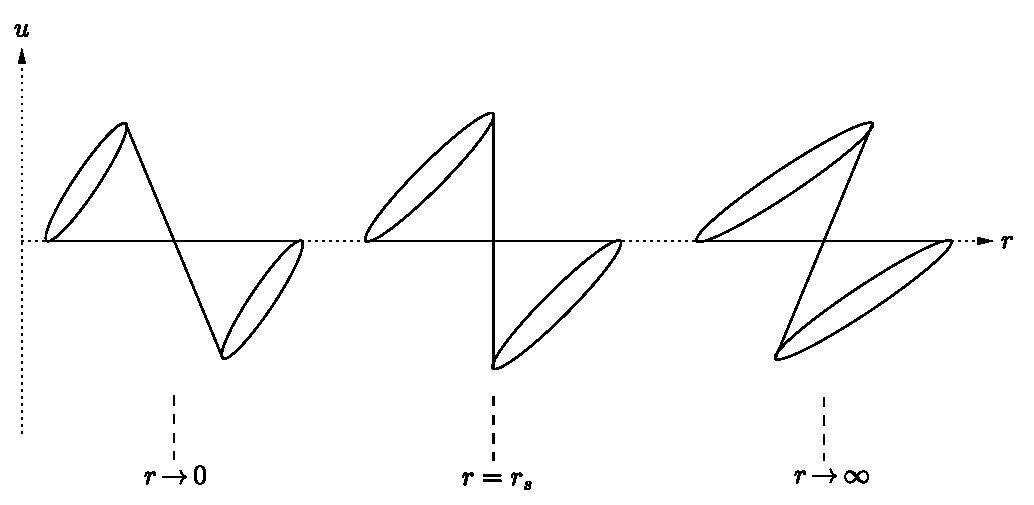
\includegraphics[width=0.65\textwidth]{figures/lightcones_eventhorizon.pdf}
	\caption{Lightcones for the Eddington-Finkelstein coordinates and radial null wordlines (geodesics).}
	\label{fig:lightcones_eventhorizon}
\end{figure}
As one can see, there is no way for an event at $r \in [0,r_s]$ to develop such that information on the event travels in positive $r$-direction. This means, the surface at $r=r_s=2m$ marks a boundary, from where no information can escape; this is the so-called event horizon. The notion of the event horizon defines a black hole, which is defined as an object massive enough to have a well-defined event horizon.

% see section 27.5 pp 608
}

%\Que{How do the lightcones look in Eddington-Finkelstein coordinates, as $r \rightarrow r_s \rightarrow 0$?}
%\Ans{
%Text. % pages 609-611
%}

\section{Black holes}
\Que{How can a black hole be defined with respect to the event horizon located at the Schwarzschild radius $r_s=2m$?}
\Ans{
The Schwarzschild radius $r_s$ is a natural length quantity arising from the Schwarzschild metric, which describes mass distributions which are spherically symmetric, uncharged and non-rotating. As one can derive from the Schwarzschild metric in Eddington-Finkelstein coordinates, the Schwarzschild radius marks a boundary, from where no information can escape; the so-called event horizon.

A black hole is any object, for which the actual physical extent $r_0$ is less than the event horizon, meaning that entities can pass beyond the event horizon towards the massive object. Mathematically speaking, a black hole is defined by a spherical mass distribution of total mass $M$ and radius $r_0$, such that $r_0 < r_s = 2m$ holds, where $m = MG_N/c^2$. Assuming for simplicity a constant mass density $\rho_0$ of the object, the requirement $r_0 < r_s$ translates into a requirement for a sufficiently large density, namely \begin{equation}
	\left(\frac{3}{4\pi\rho_0}\right)^{1/3} < 2\frac{G_N M^{2/3}}{c^2}.
\end{equation} Exponentiating this expression by $3$ yields \begin{equation}
\frac{3}{4\pi\rho_0} < 8\frac{G_N^3 M^2}{c^6},
\end{equation} from which further \begin{equation}
\frac{1}{\rho_0} < q\cdot M^2, \quad q \doteq \frac{32\pi G_N^3}{3c^6}
\end{equation} can be derived. Any object fulfilling this requirement can be called a black hole.

Expressed in words, one can define a black hole as an object, whose physical extent does at no position in spacetime reach or exceed its event horizon. % See eigenchris video 108d (beginning 5 minutes)
}

\Que{Which metric(s) can be used to study black holes and why?}
\Ans{
Consider the Schwarzschild radius $r_s = 2m = 2\frac{MG_N}{c^2}$, where $M$ is the mass of an object and $G_N$ is the universal constant of gravity. A black hole can be defined as any object of mass $M$, which has an actual physical extent $r_0 < r_s$. This means, that the event horizon is outside the object and hence no information can escape from such an object. In order to study such objects with extents close to the Schwarzschild radius $r_s$ it is crucial, that the used coordinates do not have a singularity at this point. The Schwarzschild coordinates are suitable to describe black holes, but only in so-called Eddington-Finkelstein coordinates. These coordinates lift the singularity at $r_s$; hence these are ideal coordinates to study black holes.
}

%\Que{How can the Eddington-Finkelstein and the Painlevé-Gullstrand metric/coordinates be discovered from a coordinate transformation of the Schwarzschild metric?}
%\Ans{
%Text. Transform time $t$ as $T(t,r) = t + \psi(r)$. Note, that $T(t,r)$ is the proper time of geodesic observers with energy $E=1$. % Section 7.2, p. 593ff
%}

%\Que{What are Kruskal-Szekeres coordinates? Why are they useful?}
%\Ans{
%Text.
%}
%
%\Que{How can the Kruskal-Szekeres universe be drawn? Which regions are there and how are they interpreted?}
%\Ans{
%Kruskal diagram. % Fig. 20, p. 621ff
%}
%
%\Que{How can the gravitational collapse of a star by accounted for by a simple model?}
%\Ans{
%Text. % p. 652ff
%}

\section{Curvature}
\Que{What is - roughly speaking - a manifold, and what does it have to do with curvature?}
\Ans{
Roughly speaking, one can understand a manifold as a curved space, which looks flat in a small local region. For example, a sphere like the surface of the earth is curved, but looks locally flat as one stands at his or her home and looks to the horizon. A sphere hence is called a two-dimensional manifold immersed in three-dimensional euclidean space. Another example would be a torus, which is also a two-dimensional manifold in $\mathbb{R}^3$. % See eigenchris video 107b
}

\Que{What is the intuition behind curvature?}
\Ans{
Curvature basically describes a property of an $n-1$ dimensional subspace of an $n$ dimensional space. Curvature can be measured in any dimension by the so-called Riemann curvature tensor. The Riemann tensor detects curvature of a so-called manifold by means of holonomy. A manifold is a possibly curved space, which in a small enough region (infinitesimal) looks like flat space. Given a closed path in a space which is to be tested for curvature, a holonomy not equal to zero indicates that the tested space is indeed curved. Holonomy is the property of a vector parallel transported around a closed path in the tested space not being the same vector before and after the parallel transport. If the holonomy of a vector in some space is non-zero, it indicates that the space is curved. Hence, holonomy provides a basic intuition for curvature.
}


\Que{What is the Riemann curvature tensor and how is it derived and defined? What basic properties does it have?}
\Ans{
The Riemann curvature tensor is a mathematical tool that measures the curvature of a four-dimensional space, namely that of spacetime. However, it could be generalized to arbitrary dimensions. In four-dimensional spacetime, it contains $4^4 = 256$ entries. Its working principle may be understood as follows: Consider two four-(co)vectors $v_\alpha$ and $w_\beta$ and a third (co)vector $t_\gamma$ in a spacetime, whose curvature shall be ``measured''. The Riemann curvature tensor is a measure for curvature of that spacetime insofar, as it gives the difference $t_\gamma - t^{\prime}_{\gamma}$, where $t^{\prime}_{\gamma}$ is the parallel transported covector $t_\gamma$ around a parallelogram spanned by the covectors $v_\alpha$ and $w_\beta$. This explains, why the Riemann curvature tensor $R^\delta_{\gamma\alpha\beta}$ consists of four indices and hence of 256 entries.

Mathematically speaking, the tensor is derived from differential geometry and is defined as \begin{equation}
	R^\lambda_{\sigma\mu\nu} = \partial_\mu\Gamma^\lambda_{\sigma\nu} - \partial_\nu \Gamma^\lambda_{\sigma\mu} + \Gamma^\lambda_{\mu\rho}\Gamma^\rho_{\nu\sigma} - \Gamma^\lambda_{\nu\rho}\Gamma^\rho_{\mu\sigma},
\end{equation} where $\Gamma^{\alpha}_{\beta\gamma}$ are the Christoffel symbols. It has the properties \begin{equation}
R_{\rho\nu\sigma\mu} + R_{\rho\mu\nu\sigma} + R_{\rho\sigma\mu\nu} = 0, \quad R_{\sigma\rho\mu\nu} = -R_{\rho\sigma\mu\nu}, \quad R_{\rho\sigma\nu\mu} = -R_{\rho\sigma\mu\nu}, \quad R_{\mu\nu\rho\sigma} = R_{\rho\sigma\mu\nu}.
\end{equation} Exploiting those symmetries notably introduced by the symmetries of the metric tensor $g^{\mu\nu}$ by means of the Christoffel symbols, it turns out that the Riemann curvature tensor only has 20 independent components in four-dimensional spacetime.% p. 216ff or eigenchris videos
}

\Que{What are the Ricci tensor and scalar and how are they derived?}
\Ans{
The Ricci (curvature) tensor $R_{\mu\nu}$ can be understood as kind of a ``summary'' of the Riemann tensor $R^\rho_{\sigma\mu\nu}$. It is defined by the contraction of the Riemann curvature tensor with itself, namely \begin{equation}
R_{\mu\nu} \doteq R^\rho_{\mu\rho\nu}.
\end{equation} One could as, why one contracts the Riemann tensor with the middle lower index, not with the left or right lower index. The answer to this is that the latter contractions would not lead to meaningful results, as it turns out that $R^\rho_{ho\alpha\beta} = -R^\sigma_{\sigma\alpha\beta} = 0$ and $R^\rho_{\alpha\beta\rho} = -R^\rho_{\alpha\rho\beta}$ holds; hence the latter first case results in zero and the latter second case in just the negative of the above defined Ricci tensor. Those contractions therefore do not lead to meaningful results, which is why the Ricci tensor is defined as it is.

The Ricci tensor is derived from the Riemann curvature tensor and has the property $R_{\alpha\beta} = R_{\beta\alpha}$; it is symmetric. Because it is symmetric, it only consists of 10 independent components.

The physical interpretation of the Ricci tensor is that it measures how a ``volume'' $V \subseteq \mathbb{R}^{n-1}$ in a space $\mathbb{R}^n$ changes along geodesics. Geodesics describe the natural trajectories of objects in general relativity; and they are the shortest possible ways on the curved spacetime from points $A$ to $B$.

The Ricci scalar $R$ is defined as \begin{equation}
	R \doteq g^{\mu\nu}R_{\mu\nu} = R^{\alpha}_\alpha,
\end{equation} where $g^{\mu\nu}$ is the metric tensor. The interpretation is that if one has a circle both in a flat space and a one of the same circumference in the curved space, the circle will have more area in flat space if $R < 0$ and conversely less are as in the curved space, if $R > 0$. % p. 224 or eigenchris videos
}


\Que{What is the curvature (Ricci tensor, Ricci scalar and Riemann tensor) of a sphere in 3D?}
\Ans{
Consider first the line element $\mathrm{d}s^2$ in polar coordinates. It can be derived from the line element $\mathrm{d}s^2 = \mathrm{d}x^2 + \mathrm{d}y^2  + \mathrm{d}z^2$ via the definition of the polar coordinates \begin{equation}
	x(r,\theta,\varphi) = r\cos(\varphi)\sin(\theta), \quad y(r,\theta,\varphi) = r\sin(\varphi)\sin(\theta), \quad z(r,\theta,\varphi) = r\cos(\theta)
\end{equation}	and the total derivatives such as \begin{equation}
\mathrm{d}x = \frac{\partial x}{\partial r}\mathrm{d}r + \frac{\partial x}{\partial \theta}\mathrm{d}\theta + \frac{\partial x}{\partial \varphi}\mathrm{d}\varphi.
\end{equation} The line element in polar coordinates for a radius $r$ thus is given by \begin{equation}
\mathrm{d}s^2 = r^2\mathrm{d}\theta^2 + r^2\sin^2(\theta)\,\mathrm{d}\varphi^2.
\end{equation}
	
	Now, the only non-zero Christoffel symbols for this metric are
	\begin{align}\begin{aligned}
		\Gamma^\theta_{\phi \phi} &= -\sin\theta \cos\theta \\
		\Gamma^\phi_{\theta \phi} &= \Gamma^\phi_{\phi \theta} = \cot\theta,
	\end{aligned}\end{align} as the Christoffel symbols are calculated using the equation 
	\begin{equation}
			\Gamma^{\mu}_{\nu\lambda} = g^{\mu\rho}\Gamma_{\rho\nu\lambda} = g^{\mu\rho}\frac{1}{2}\left(g_{\rho\nu,\lambda} + g_{\rho\lambda,\nu}-g_{\nu\lambda,\rho}\right),
	\end{equation} where $g_{\rho\nu,\lambda} = \frac{\partial g_{\rho\nu}}{\partial x^\lambda}$.
	
	The Riemann tensor for a 2-sphere has only one independent component, which is
	\begin{equation}
		R^\theta_{\phi \theta \phi} = R_{\theta \phi \theta \phi} = r^2 \sin^2\theta.
	\end{equation} Therefore, the full Riemann tensor can be written as
	\begin{equation}
		R_{\mu\nu\rho\sigma} = \frac{1}{r^2} (g_{\mu\rho} g_{\nu\sigma} - g_{\mu\sigma} g_{\nu\rho}).
	\end{equation}
	
	Moving on to the Ricci tensor \( R_{\mu\nu} \), according to its definition it is obtained by contracting the Riemann tensor. For the 2-sphere, it is proportional to the metric
	\begin{equation}
		R_{\mu\nu} = \frac{1}{r^2} g_{\mu\nu}.
	\end{equation} Explicitly, the components are
	\begin{align}\begin{aligned}
		R_{\theta\theta} &= 1 \\
		R_{\phi\phi} &= \sin^2\theta.
	\end{aligned}\end{align}
	
	Finally, the Ricci scalar $R$ is obtained by contracting the Ricci tensor. For the 2-sphere, it is given by
	\begin{equation}
		R = g^{\mu\nu} R_{\mu\nu} = \frac{2}{r^2}.
	\end{equation} This provides a link to Gaussian curvature $K$, which can be defined as \begin{equation}
	K = -R/2,
	\end{equation} where $R$ is the Ricci scalar. Hence, the Gaussian curvature for the sphere can be accounted for by $K = -1/r^2$, which matches the expectation from differential geometry.
}

\Que{How can it be shown easily, that some metric $g_{\alpha\beta}(x)$ in some coordinates $x^\alpha$ is not the Minkowski metric?}
\Ans{
Calculate the Riemann curvature tensor. If not all components are zero, $x^\alpha$ do not describe Minkowski space, since Minkowski spacetime is flat. A tensor being zero does not depend on different coordinate systems, since the tensor is just multiplied by Jacobi matrices if a transformation $x^\alpha \rightarrow y^\mu$ is performed.
}

\Que{How can curvature of spacetime intuitively be explained?}
\Ans{
Curvature of spacetime can either be understood by geodesic deviation or holonomy.

The ansatz with geodesic deviation says that neighbouring geodesics diverge or converge depending on the point in space under consideration. It just means, that geodesics are not separated from one another homogeneously at same distances throughout the spacetime.

The ansatz with holonomy captures curvature as the deviation of a vector prior and posterior to being parallel transported around a closed trajectory in the spacetime. If the spacetime is curved, then the parallel transported vector will not be the same posterior to its transportation as compared to prior to the parallel transport. This is called holonomy. Therefore, a spacetime is curved, if it consists of holonomy, and flat, if there is no holonomy in the spacetime. % See eigenchris videos
}

\section{Einstein field equations}
\Que{How is the Poisson equation of gravity derived?}
\Ans{
Consider Newton's law of gravity for two pointlike masses $M_1$ and $M_2$ separated by a distance $r$ given by the vector $\vect{r}$ pointing from $M_1$ to $M_2$. The attractive gravitational force $\vect{F}$ between both bodies is given by \begin{equation}
	\vect{F} = G_N\frac{M_1M_2}{r^3}\vect{r} = G_N \frac{M_1M_2}{r^2}\vect{e}_r,
\end{equation} where $\vect{e}_r$ is a unit vector in the direction of $\vect{r}$. Identifying the mass $M_1$ as the source of gravity, one can also write the force $\vect{F}$ by means of the product of the mass $M_2$ with the gravitational field $\vect{g}$ given by \begin{equation}
\vect{F} = -M_2 \vect{g}(r) = M_2 G_N \frac{M_1}{r^2}\vect{e}_r.
\end{equation} Hereby, $\vect{g}(r)$ is the gravitational field introduced by the mass $M_1$. One can write $M_1$ as $M_r$ with \begin{equation}
M_r = \int_{V(r)} \rho(\vect{r})\,\mathrm{d}V= \int_{\varphi=0}^{2\pi}\mathrm{d}\varphi \int_{\theta=-\pi/2}^{\pi/2}\mathrm{d}\theta \sin(\theta) \int_{r^\prime=0}^{r}r^{\prime \, 2}\rho(\vect{r}(r^\prime, \theta,\varphi))\,\mathrm{d}r^\prime
\end{equation} in the general case, where $V(r)$ denotes a spherical volume of radius $r$. The mass density is denoted by $\rho(\vect{r})$, where $\vect{r}$ points from the origin of the coordinate system to any point of mass in the volume.

Now, the gravitational field $\vect{g}(r)$ of a mass distribution described by the mass density $\rho(\vect{r})$ enclosed by a radius $R \leq r$ at a point $r$ radially away from the mass distribution is given by \begin{equation}
	\vect{g}(r) = -G_N\frac{M_r}{r^2}\vect{e}_r = -\frac{G_N}{r}\left(\int_{V(r)}\rho(\vect{r})\,\mathrm{d}V\right)\vect{e}_r.
\end{equation} Since gravitational fields are conservative force fields, one can write $\vect{g}$ as the gradient of a scalar potential, namely \begin{equation}
\vect{g}(r) = -\vect{\nabla}\phi(r)
\end{equation} with a scalar potential \begin{equation}
\phi(r) = -G_N\frac{M_r}{r}.
\end{equation} Now, the integral theorem of Gauss states for a vector field $\vect{U}$ meeting the appropriate mathematical requirements, the relation \begin{equation}
\int_{\partial V} \vect{U}\cdot \mathrm{d}\vect{S} = \int_{V} \vect{\nabla}\cdot \vect{U}\,\mathrm{d}V
\end{equation} holds, there $\partial V$ is the surface enclosing the volume $V$ and $\mathrm{d}\vect{S}$ is a vectorial surface element on $\partial V$. This theorem is applicable for the gravitational field $\vect{g}(r)$; hence we have \begin{equation}
\int_{\partial V(r)} \vect{g}(r)\cdot \mathrm{d}\vect{S} = \int_{V(r)} \vect{\nabla}\cdot \vect{g}(r)\,\mathrm{d}V.
\end{equation} The first term is evaluated as \begin{align}\begin{aligned}
\int_{\partial V(r)} \vect{g}(r)\cdot \mathrm{d}\vect{S} &= -G_NM_r\int_{\partial V(r)}\frac{1}{r^2}\vect{e}_r\cdot\vect{e}_rr^2\sin(\theta)\,\mathrm{d}\theta\,\mathrm{d}\varphi \\
&= -G_NM_r\int_{\varphi=0}^{2\pi}\mathrm{d}\varphi\int_{\theta=-\pi/2}^{\pi/2}\sin(\theta)\,\mathrm{d}\theta = -4\pi G_NM_r \\ &= -4\pi G_N \int_{V(r)} \rho(\vect{r})\,\mathrm{d}V .
\end{aligned}\end{align} The second part of the above Gauss theorem relation is accounted for by \begin{equation}
\int_{V(r)}\vect{\nabla}\cdot \vect{g}(r)\,\mathrm{d}V = -\int_{V(r)}\vect{\nabla}\cdot\vect{\nabla}\phi(r)\,\mathrm{d}V = -\int_{V(r)}\Delta \phi(r)\,\mathrm{d}V.
\end{equation} Making now use of the Gauss theorem equation and relating both terms yields \begin{equation}
-4\pi G_N \int_{V(r)} \rho(\vect{r})\,\mathrm{d}V = -\int_{V(r)}\Delta \phi(r)\,\mathrm{d}V \quad \Leftrightarrow \quad \Delta \phi = 4\pi G_N \rho.
\end{equation} Hence, a gravitational field is in Newtonian gravity accounted for by the so-called Poisson equation \begin{equation}
\Delta \phi(\vect{r}) = 4\pi G_N \rho(\vect{r}),
\end{equation} where $\vect{r}$ is the position vector of any point of mass given by the mass density $\rho(\vect{r})$, $\Delta = \vect{\nabla} \cdot \vect{\nabla}$ is the Laplace operator, $\phi(\vect{r})$ is the gravitational potential and $G_N$ is the universal constant of gravity.
}

\Que{How is the energy-momentum tensor $T_{\alpha\beta}$ in general relativity defined/derived? What does it describe/mean?}
\Ans{
The energy-momentum tensor is a generalization of the mass density $\rho$ in the Poisson equation $\Delta \phi = 4\pi G_N\rho$ to any frame of reference in special and general relativity. The key here is that the mass density $\rho$ is not Lorentz-invariant; this can be seen by imagining a cube moving in the x-direction of the coordinate system such that its length in the x-direction is contracted by half its rest length size. This would mean that the mass density $\rho$ would be $2\rho$ in the moving reference frame as compared to $\rho$ in the rest reference frame. The energy-momentum tensor comes in here to serve as a Lorentz-invariant generalization for the mass density in general relativity. It is defined such that it tracks the flux of energy-momentum through spacetime. % see p. 203ff or eigenchris video 107e Energy momentum is the generalization of mass density for 4-d spacetime and Lorentz-invariant?

Now, the energy-momentum tensor $T^{\alpha\beta}$ ``counts'' the momentum ``flowing'' through a 3D unit volume of spacetime. If $N^\alpha$ would denote the flux of particles through a 3D unit volume of spacetime, the energy-momentum tensor $T^{\alpha\beta}$ requires an additional dimension, since one now counts momentum (vector $p^{\alpha}$) per unit volume instead of particles. Hence, the energy-momentum tensor $T^{\alpha\beta}$ can heuristically be defined as the flux (current density) of $\alpha$-momentum going through a 3D unit volume of constant $\beta$. Mathematically, this can be expressed by means of \begin{align}
	\begin{aligned}
		T^{\alpha t} = \frac{p^\alpha}{\mathrm{d}x\,\mathrm{d}y\,\mathrm{d}z}, \quad T^{\alpha x} = \frac{p^{\alpha}}{c\,\mathrm{d}t\,\mathrm{d}y\,\mathrm{d}z}, \quad T^{\alpha y} = \frac{p^{\alpha}}{c\,\mathrm{d}t\,\mathrm{d}x\,\mathrm{d}z}, \quad T^{\alpha z} = \frac{p^{\alpha}}{c\,\mathrm{d}t\,\mathrm{d}x\,\mathrm{d}y},
	\end{aligned}
\end{align} where $\alpha \in \{t,x,y,z\}$. Taking a closer look at the individual components, one can see that some entries are just energy or momentum densities (energy or momentum divided by 3D space), whereas others are energy or momentum fluxes (energy or momentum divided by time and 2D area). Consider \cref{fig:energymomentum} for a visualization of this.
\begin{figure}[h]
	\centering
	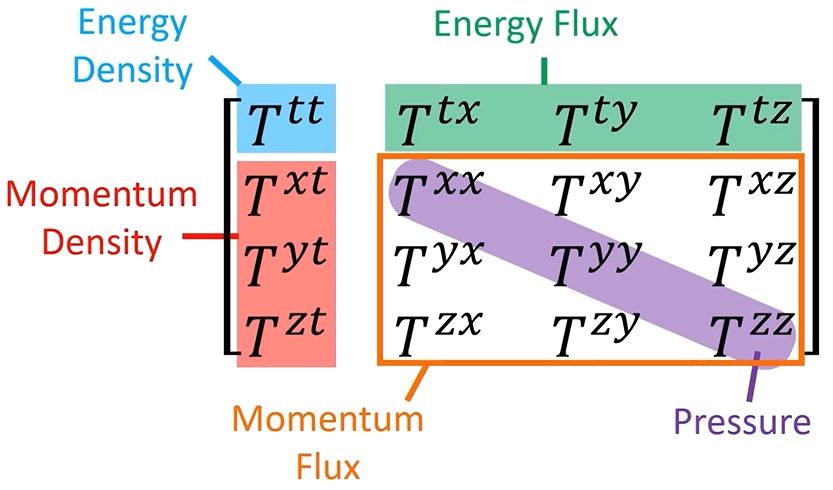
\includegraphics[width=0.4\textwidth]{figures/energymomentum.png}
	\caption{Energy-momentum tensor $T^{\alpha\beta}$ and the nature of its individual entries. Recall, that the energy-momentum tensor $T^{\alpha\beta}$ gives the flux of $\alpha$-momentum going through a 3D unit volume of constant $\beta$. Note therefore, that the $T^{xx}$, $T^{yy}$ and $T^{zz}$ components are pressures in nature; that is, momentum divided per time and area.}
	\label{fig:energymomentum}
\end{figure}
}

%\Que{What is the commutator of covariant derivatives, how is it defined and why is it important in deriving/describing curvature of spacetime?}
%\Ans{
%Text. % p. 216ff
%}  

\Que{What is Newton-Cartan theory, what are the main steps in the derivation and what is the key result of it?}
\Ans{
Newton-Cartan theory is a general-relativity-like description of Newtonian gravity. General relativity is described by a curved spacetime, geodesics, Lorentz transformations and the proper time $\tau$. Newton-Cartan theory however uses Galilean transformations and universal time $t$, as compared to general relativity. With that, it aims to bridge the gap between Newtonian gravity and general relativity.

In order to derive Newton-Cartan theory, one starts with the classical Newtonian equation \begin{equation}
	m\vect{a} = \vect{F}_g = m\vect{g} = -\vect{\nabla}\phi,
\end{equation} where $m$ is the mass, $\vect{a} = \mathrm{d}^2\vect{x}/\mathrm{d}t^2$ the acceleration vector and $\vect{F}_g$ the gravitational force exerted by the gravitational field on the mass $m$. Hereby, $\vect{g}$ furthermore is the gravitational field describable by the gravitational potential $\phi$ usually given by $\phi = -G_Nm/r$, where $r$ is the radial coordinate of a spherically symmetric potential.

Now, employing the convention, that latin letters denote spatial components and greek letters spatial and temporal components of a four vector, the above Newtonian equation can be written as \begin{equation}
	\frac{\mathrm{d}^2x^i}{\mathrm{d}t^2} + \frac{\partial \phi}{\partial x^i} = 0.
\end{equation} The next step then is to determine the connection coefficients (Christoffel symbols) $\Gamma^\sigma_{\mu\nu}$ to match this equation to the geodesic equation \begin{equation}
\frac{\mathrm{d}^2x^\sigma}{\mathrm{d}\lambda^2} + \Gamma^\sigma_{\mu\nu}\frac{\mathrm{d}x^\mu}{\mathrm{d}\lambda}\frac{\mathrm{d}x^\nu}{\mathrm{d}\lambda} = 0.
\end{equation} Performing the substitution $\lambda \rightarrow t$ in the geodesic equation, one finds after some tedious calculations that \begin{equation}
\Gamma^i_{00} = \frac{\partial \phi}{\partial x^i}, \quad \Gamma^0_{\mu\nu} = \Gamma^i_{jk} = \Gamma^i_{0k} = \Gamma^i_{j0} = 0.
\end{equation} Using this result to calculate the Riemann curvature, one finds that the only nonzero components are \begin{equation}
R^i_{0j0} = -R^i_{00j} = \partial_j\partial_i\phi,
\end{equation} which thus is a tensor with 9 components and 6 independent components. Moving on to calculate the Ricci tensor $R_{\mu\nu}$, the result is that the only nonzero component is $R_{00}$ given by \begin{equation}
R_{00} = R^\mu_{0\mu 0} = R^0_{000} + R^1_{111} + R^2_{222} + R^3_{333} = 0 + \partial_1\partial_1 \phi + \partial_2\partial_2 \phi + \partial_3\partial_3 \phi = \Delta \phi = 4\pi G_N \rho.
\end{equation} This result now suggests, that the mass density $\rho$ must be the part $T_{00}$ of a general four by four tensor $T_{\mu\nu}$, just as $R_{00}$ is the zero-zero component of the four by four tensor called the Ricci tensor $R_{\mu\nu}$; that is, the equation \begin{equation}\label{eq:newtoncartan}
R_{00} = 4\pi G_N T_{00}
\end{equation} is proposed, which is the main result of Newton-Cartan theory.
}

\Que{How are the Einstein field equations derived?}
\Ans{
Now, from the Newton-Cartan theory result derived above, one could propose the generalized equation \begin{equation}
	R^{\mu\nu} \overset{?}{=} \kappa T^{\mu\nu},
\end{equation} where $\kappa$ would be any constant of proportionality. It can however be derived using tedious calculations, that the covariant divergence of the energy-momentum tensor $T^{\mu\nu}$ is \begin{equation}
\nabla_\mu T^{\mu\nu} = \partial_\mu T^{\mu\nu} + \Gamma^\mu_{\mu\lambda} T^{\lambda\nu} = 0,
\end{equation} while the covariant divergence of the Ricci tensor $R^{\mu\nu}$ is \begin{equation}
\nabla_\mu R^{\mu\nu} = \partial_\mu R^{\mu\nu} + \Gamma^\mu_{\mu\lambda} R^{\lambda\nu} \neq 0.
\end{equation} Thus, the above proposed equation is not true, i.e. $R^{\mu\nu} \neq \kappa T^{\mu\nu}$. It can however be proven, that the covariant divergence of the so-called Einstein tensor $G^{\mu\nu}$ defined as \begin{equation}
G^{\mu\nu} \doteq R^{\mu\nu} - \frac{1}{2}Rg^{\mu\nu}
\end{equation} results in \begin{equation}
\nabla_\mu G^{\mu\nu} = \partial_\mu G^{\mu\nu} + \Gamma^\mu_{\mu\lambda} G^{\lambda\nu} = 0.
\end{equation} Thus, one can formulate the proposition \begin{equation}
R^{\mu\nu} - \frac{1}{2}Rg^{\mu\nu} = \kappa T^{\mu\nu}
\end{equation} for the Einstein field equations. Note however, that can make a slight modification, as the derivative of any function $f(x)$ with respect to $x$ does not change, if a constant $c$ is added to the function $f(x)$. This means, that one can add to Einstein tensor a constant $\Lambda$, since if $\nabla_\mu G^{\mu\nu} = 0$, then also $\nabla_\mu (G^{\mu\nu} + \Lambda g^{\mu\nu})$ must hold (because $\nabla_\mu g^{\mu\nu} = 0$). Furthermore, the proportionality constant $\kappa$ is derived to be $\kappa = 8\pi G_N/c^4$. Thus, the full Einstein field equations can be written as \begin{equation}
R^{\mu\nu} - \frac{1}{2}Rg^{\mu\nu} + \Lambda g^{\mu\nu} = \frac{8\pi G_N}{c^4}T^{\mu\nu}.
\end{equation} Note, that one sometimes also gives this equation in units $c=1$. Hereby, $R^{\mu\nu}$ is the Ricci tensor, $g^{\mu\nu}$ is the metric tensor, $R$ is the Ricci scalar, $G_N$ is the universal constant of gravity, $\Lambda$ is the cosmological constant, $c$ is the speed of light and $T^{\mu\nu}$ is the energy-momentum tensor.

The proofs of $\nabla_\sigma g^{\mu\nu} = 0$, $\nabla_\mu T^{\mu\nu}$ and $\nabla_\mu G^{\mu\nu}$ are tedious, but not very instructive; one just has to perform the calculations, which are lengthy, but not difficult in the sense of argumentation - just by-the-book calculations. However, the derivation of the constant of proportionality $\kappa = 8\pi G_N/ c^4$ is more instructive. This constant is derived by forcing the Einstein field equations to reduce to Poisson's equation in the limit of low velocities, weak gravity and a time-independent metric $g^{\mu\nu}$.


\Que{What does it mean to ``solve'' the Einstein field equations?}
\Ans{
To solve the Einstein field equations 
\begin{equation}
	R_{\mu\nu} - \frac{1}{2}Rg_{\mu\nu} + \Lambda g_{\mu\nu} = \frac{8\pi G_N}{c^4}T_{\mu\nu}.
\end{equation}
means that one puts in an energy-momentum tensor $T_{\mu\nu}$ for a particular system under consideration and solves for the metric $g_{\mu\nu}$. The metric is a description of the geometry of spacetime and thus gives the gravitational behaviour. From the metric, all the curvature properties of the spacetime can be derived. Furthermore, using the metric, one can obtain the Christoffel symbols and solve the geodesic equation giving the paths of masses and light in the gravitational field described by the metric $g_{\mu\nu}$.
}


% see eigenchris videos, p. 374ff
}

%\Que{How are the Einstein field equations formally derived?}
%\Ans{
%Text. % see eigenchris videos, p. 374ff
%}

%\Que{What is the Einstein-Hilbert action and what can it be used for?}
%\Ans{
%Text. % pp 388ff
%}

%\Que{What is the  Gibbons-Hawking-York boundary term?}
%\Ans{
%Text. % pp 397ff
%}

%\Que{What are the Bianchi identities and why are they significant to general covariance?}
%\Ans{
%Text. % pp. 385ff
%}

\subsection{Deriving the Schwarzschild metric as a solution to the Einstein field equations}
\Que{How is the Schwarzschild metric derived from the Einstein field equations in a vacuum?}
\Ans{
The Schwarzschild metric is obtained from solving the Einstein field equations for a particular set of conditions. It turns out that the Schwarzschild metric is very useful for describing e.g. the exterior of non-rotating black holes or the gravitational field of general massive bodies and the behaviour of objects present in this gravitational field.

The set of conditions to obtain the Schwarzschild metric from the Einstein field equations is given by the following:	
\begin{enumerate}
	\item The system is assumed to exhibit spherical symmetry and a static spacetime, meaning $\partial_t g_{\mu\nu} = 0$ and $t \rightarrow -t$ does not change $g_{\mu\nu}$.
	\item Only the region outside a mass distribution described by the mass density $\rho$ is considered, meaning that the energy-momentum tensor $T_{\mu\nu} = 0$, as the space outside a mass distribution is approximately a vacuum.
	\item As one moves far away from the mass distribution $\rho$, the effects of gravity become negligible, meaning that spacetime is approximately flat and hence $g_{\mu\nu}\approx \eta_{\mu\nu}$, where $\eta_{\mu\nu}$ is the Minkowski metric.
	\item The scale of the system is non-cosmological, meaning that $\Lambda \approx 0$.
\end{enumerate}
	
First, one can see, that under the assumptions $T_{\mu\nu} = 0$ and $\Lambda = 0$, the Einstein field equations simplify to just $R_{\mu\nu} = 0$, because 
\begin{equation}
	R_{\mu\nu} - \frac{1}{2}Rg_{\mu\nu} = 0 \quad \Leftrightarrow \quad g^{\mu\nu}R_{\mu\nu} = \frac{1}{2}Rg^{\mu\nu}g_{\mu\nu} \quad \Leftrightarrow \quad R = 4\frac{1}{2}R \quad \Leftrightarrow \quad R = 0
\end{equation} and thus $R_{\mu\nu} = 0$, if one inserts $R=0$ back into the first relation of the above equation line.

Now, since a Schwarzschild metric is spherically symmetric, one uses spherical coordinates $x^\mu = (ct, r, \theta,\varphi)$. In flat spacetime, the metric $g_{\mu\nu}$ in spherical coordinates would by given by just \begin{equation}
	g_{\mu\nu} = \begin{pmatrix}
		-1 & 0 & 0 & 0 \\
		0 & 1 & 0 & 0 \\
		0 & 0 & r^2 & 0 \\
		0 & 0 & 0 & r^2\sin^2(\theta)
	\end{pmatrix}
\end{equation} in the mostly plus convention, as the line element is $\mathrm{d}s^2 = g_{\mu\nu}\,\mathrm{d}x^\mu\,\mathrm{d}x^\nu = -c^2\,\mathrm{d}t^2 + \mathrm{d}r^2 + r^2\,\mathrm{d}\theta^2 + r^2\sin^2(\theta)\,\mathrm{d}\varphi^2$ for spherical coordinates. Since the expected metric describes a curved spacetime, we propose the general metric \begin{equation}
	g_{\mu\nu} = \begin{pmatrix}
		g_{tt} & g_{tr} & g_{t\theta} & g_{t\varphi} \\
		g_{rt} & g_{rr} & g_{r\theta} & g_{r\varphi} \\
		g_{\theta t} & g_{\theta r} & g_{\theta\theta} & g_{\theta\varphi} \\
		g_{\varphi t} & g_{\varphi r} & g_{\varphi \theta} & g_{\varphi\varphi}
	\end{pmatrix}
\end{equation} to begin with.

For the remaining material of this answer, latin super-or subscripts will denote only spatial components. The condition of a static metric means that a time reversal $t \rightarrow -t$ shall not change the metric $g_{\mu\nu}$. As the components of the metric $g_{\mu\nu}$ are given by $g_{\mu\nu} = \partial_\mu\partial_\nu$, this means that \begin{equation}
	g_{tt} = \frac{\partial}{\partial c t} \frac{\partial}{\partial c t} \rightarrow \frac{\partial}{\partial (- c t)} \frac{\partial}{\partial (-c t)} = g_{tt},
\end{equation} but also \begin{equation}
g_{ti} = g_{it} =  \frac{\partial}{\partial c t}\partial_i \rightarrow \partial_i \frac{\partial}{\partial (-ct)} = -g_{ti} = -g_{it} = 0.
\end{equation} Thus, the metric has already reduced to \begin{equation}
g_{\mu\nu} = \begin{pmatrix}
	g_{tt} & 0 & 0 & 0 \\
	0 & g_{rr} & g_{r\theta} & g_{r\varphi} \\
	0 & g_{\theta r} & g_{\theta\theta} & g_{\theta\varphi} \\
	0 & g_{\varphi r} & g_{\varphi \theta} & g_{\varphi\varphi}
\end{pmatrix}.
\end{equation} In order to fulfill spherical symmetry furthermore, the components $g_{\theta\varphi} = g_{\varphi\theta}$ need to be zero, but $g_{\theta\theta}$ and $g_{\varphi\varphi}$ to be those of the flat metric in spherical coordinates. In addition to this, also $g_{\theta r} = g_{r\theta}$ and $g_{\varphi r} = g_{r\varphi}$ need to go to zero, if one wants $\vect{e}_\theta \perp \vect{e}_r$ aswell as $\vect{e}_\varphi \perp \vect{e}_r$. At this stage, the metric looks like \begin{equation}
g_{\mu\nu} = \begin{pmatrix}
	g_{tt}(r,\theta,\varphi) & 0 & 0 & 0\\
	0 & g_{rr}(r,\theta,\varphi) & 0 & 0 \\
0& 0 & r^2 & 0 \\
	0 & 0 & 0 &  r^2\sin^2(\theta)
\end{pmatrix}.
\end{equation} The lower right two nonzero components can be multiplied by a function $C(r)$ and still maintain spherical symmetry. Furthermore, the first components cannot depend on $\theta$ and $\varphi$ while still maintaining spherical symmetry; hence one can write $g_{tt} = -A(r)$ and $g_{rr} = B(r)$. The coordinated $r$ can be just redefined to $r \rightarrow  \sqrt{C(r)}r$, yielding the form
\begin{equation}
	g_{\mu\nu} = \begin{pmatrix}
		-A(r) & 0 & 0 & 0\\
		0 & B(r) & 0 & 0 \\
		0& 0 & r^2 & 0 \\
		0 & 0 & 0 &  r^2\sin^2(\theta)
	\end{pmatrix}.
\end{equation} The remaining procedure to obtain the functions $A(r)$ and $B(r)$ is now outlined in \cref{fig:remaining}.
\begin{figure}
	\centering
	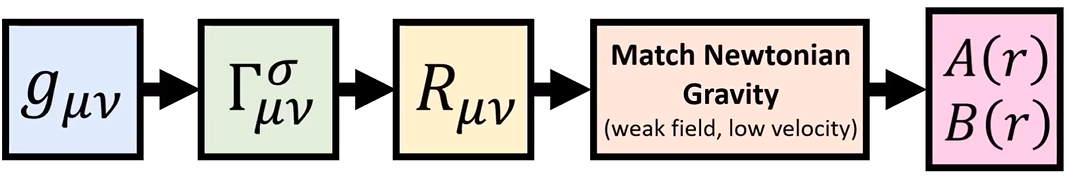
\includegraphics[width=0.5\textwidth]{figures/remaining.png}
	\caption{Outline on how to determine the functions $A(r)$ and $B(r)$ of the Schwarzschild metric.}
	\label{fig:remaining}
\end{figure} That is to say, the Christoffel symbols (connection coefficients) $\Gamma^\sigma_{\mu\nu}$ are determined from the now determined metric entries $g_{\mu\nu}$. Once the connection coefficients $\Gamma^\sigma_{\mu\nu}$ are known, the Riemann curvature tensor and hence the Ricci tensor $R_{\mu\nu}$ can be calculated. As an almost final step then, the Ricci tensor is forced to match the Ricci tensor for Newtonian gravity, which is general relativity in the limit of weak gravitational fields ($g_{\mu\nu} = \eta_{\mu\nu} + h_{\mu\nu}$ being the Minkowski metric of flat spacetime plus a small contribution $h_{\mu\nu}$) and low velocities $v \ll c$ (meaning, that Galilean transformations instead of Lorentz transformations can be used). Performing all those steps, one obtains a differential equation for $A(r)$ and $B(r)$, whose solution leads to the final form of the Schwarzschild metric. Those steps will now be performed in the following text.

\paragraph{Calculation of the $\Gamma^\sigma_{\mu\nu}$}
We start with the calculation of the connection coefficients $\Gamma^0_{\mu\nu}$, then move on to the calculations of $\Gamma^1_{\mu\nu}$, $\Gamma^2_{\mu\nu}$ and $\Gamma^3_{\mu\nu}$. The standard formula for $\Gamma^\sigma_{\mu\nu}$ is \begin{equation}
	\Gamma^\sigma_{\mu\nu} = \frac{1}{2}g^{\sigma\alpha}\left(\partial_\nu g_{\alpha\mu}+\partial_\mu g_{\alpha\nu} - \partial_\alpha g_{\mu\nu}\right).
\end{equation} Since the metric $g_{\mu\nu}$ is diagonal, the inverse metric is easily obtained by just taking the reciprocal values of the entries as \begin{equation}
g^{\mu\nu} = \begin{pmatrix}
	-\frac{1}{A(r)} & 0 & 0 & 0 \\
	 0 & \frac{1}{B(r)} & 0 & 0 \\
	 0 & 0 & \frac{1}{r^2} & 0 \\
	 0 & 0 & 0 & \frac{1}{r^2\sin^2(\theta)}
\end{pmatrix}.
\end{equation} As a first step, one notices that only the components $g^{\mu\mu}$ are nonzero, since the metric is diagonal; hence, one writes $\Gamma^\sigma_{\mu\nu} = \frac{1}{2}g^{\sigma\sigma}\left(\partial_\nu g_{\sigma\mu}+\partial_\mu g_{\sigma\nu} - \partial_\sigma g_{\mu\nu}\right).$ Now, take a look at $\Gamma^0_{\mu\nu}$, it is given by $\Gamma^0_{\mu\nu} = \tfrac{1}{2}g^{00}\left(\partial_\nu g_{0\mu} + \partial_\mu g_{0\nu} - \partial_0 g_{\mu\nu}\right)$. If both lower indexes are zero, one ends up with $\Gamma^0_{00}$ because $g_{00}$ is independent of time. For spatial lower indexes $i$, one has \begin{equation}
\Gamma_{ii}^0 = \frac{1}{2}g^{00}\left(\partial_i g_{0i} + \partial_i g_{0i} - \partial_0 g_ii\right) = 0,
\end{equation} because the first two terms in the bracket are derivatives of zero and the components $g_{ii}$ are time independent. If the lower indices are spatial, but not equal, one has \begin{equation}
\Gamma^0_{ij} = \frac{1}{2}g^{00}\left(\partial_j g_{0i}+\partial_i g_{0j}-\partial_0 g_{ij}\right) = 0,
\end{equation} since all derivative are those of off-diagonal and thus zero components. If one lower index is zero and the other spatial, we have \begin{equation}
\Gamma^0_{0i} = \Gamma^0_{i0} \frac{1}{2}g^{00}\left(\partial_i g_{00} + \partial_0 g_{0i} - \partial_0 g_{0i}\right) = \frac{1}{2}g^{00}(\partial_i g_{00}).
\end{equation} The remaining terms are spatial derivatives of $-A(r)$, where only the $r$-derivative survives; hence we have $\Gamma^{0}_{01} = \Gamma^0_{10} = \frac{1}{2A(r)}(\partial_rA(r))$. % Go on at 14:06

In a similar way, all the components of the Christoffel tensor $\Gamma^\sigma_{\mu\nu}$ can be calculated; the results for those calculations are summarized in \cref{fig:conn_coeff}.
\begin{figure}[h]
	\centering
	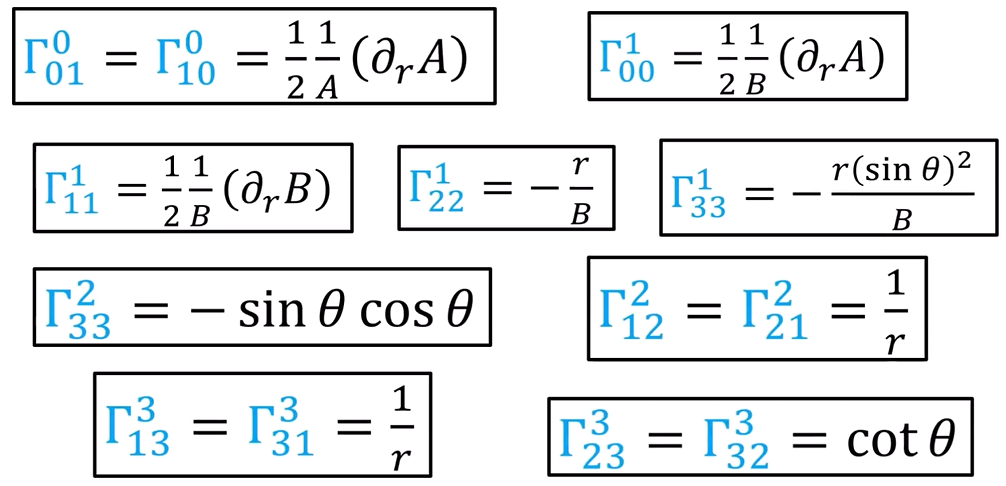
\includegraphics[width=0.5\textwidth]{figures/schwarzschild_metric_conn_coeff.png}
	\caption{Results for the connection coefficients $\Gamma^\sigma_{\mu\nu}$ for the Schwarzschild metric.}
	\label{fig:conn_coeff}
\end{figure} Note, that these equations are independent of the used sign convention for the metric tensor $g^{\mu\nu}$. Now, the next step of calculating the Ricci tensor $R_{\mu\nu}$ can be performed.

\paragraph{Calculation of the $R_{\mu\nu}$} The Ricci tensor is defined as the trace of the Riemann tensor, hence it can be written as \begin{equation}
	R_{\mu\nu} = R^\lambda_{\mu\lambda\nu} = \partial_\lambda \Gamma^{\lambda}_{\mu \nu} - \partial_\nu \Gamma^{\lambda}_{\mu \lambda} + \Gamma^{\lambda}_{\lambda \sigma} \Gamma^{\sigma}_{\mu \nu} - \Gamma^{\lambda}_{\nu \sigma} \Gamma^{\sigma}_{\mu \lambda}.
\end{equation}
Carefully substituting all the calculated non-zero Christoffel symbols into the equation for the Ricci tensor, one obtains expression for $R_{00}$, $R_{11}$ and $R_{22}$. The expression for $R_{33}$ is not necessary anymore to calculate the exact expressions for $A(r)$ and $B(r)$. It is already known from the Einstein field equations under the Schwarzschild assumptions, that $R_{\mu\nu} = 0$ holds. Performing the tedious, but straightforward task of calculating $R_{00}$, $R_{11}$ and $R_{22}$, one obtains \begin{align}\begin{aligned}
	R_{00} &= 2rABA^{\prime\prime} - rAA^\prime B^\prime + 4ABA^\prime - rB(A^\prime)^2 = 0,\\
	R_{11} &= -2rABA^{\prime\prime} + rB(A^\prime)^2 + rAA^\prime B^\prime + 4A^2B^\prime = 0, \\
	R_{22} &= -2AB+2AB^2 - rA^\prime B + rAB^\prime = 0,
\end{aligned}\end{align} where $A^\prime \doteq \partial_r A(r)$ and $B^\prime \doteq \partial_r B(r)$ was used. 

\paragraph{Calculation of the functions $A(r)$ and $B(r)$} Adding up $R_{00}$ and $R_{11}$ still must be equal to zero, so \begin{equation}
R_{00} + R_{11} = 4ABA^\prime + 4A^2B^\prime = BA^\prime + AB^\prime = 0.
\end{equation} Because $BA^\prime + AB^\prime = \partial_r(AB)$, one can conclude \begin{equation}
A(r)B(r) = K = \text{const.}
\end{equation} Now, the metric $g_{\mu\nu} = g_{\mu\nu}(r,\theta)$ must become the Minkowski metric $\eta_{\mu\nu}$ in the limit $r\rightarrow \infty$, that is to say, infinitely far from the point where the mass density $\rho$ is located. Hence we have \begin{equation}
g_{\mu\nu} = \begin{pmatrix}
	-A(r) & 0 & 0 & 0 \\
	0 & B(r) & 0 & 0 \\
	0 & 0 & r^2 & 0 \\
	0 & 0 & 0 & r^2\sin^2(\theta)
\end{pmatrix} \xrightarrow{r\rightarrow \infty} \eta_{\mu\nu} = \begin{pmatrix}
-1 & 0 & 0 & 0 \\
0 & 1 & 0 & 0 \\
0 & 0 & r^2 & 0 \\
0 & 0 & 0 & r^2\sin^2(\theta),
\end{pmatrix}
\end{equation} wherefrom it follows that $A(r\rightarrow \infty)B(r\rightarrow \infty) = 1 = K$ holds. Because $A(r)B(r) = K$ for all $r$ however, $K=1$ is true for all $r$. Therefore, we have obtained the relation \begin{equation}
A(r) = \frac{1}{B(r)}.
\end{equation} Now, inserting $B(r) = A(r)^{-1}$ alongside with $\partial_rB(r) = \partial_r(A(r)^{-1}) = -\frac{\partial_r A(r)}{A(r)^2}$ into the equation for $R_{22}$, we obtain a differential equation \begin{equation}
r\frac{\mathrm{d} A(r)}{\mathrm{d}r} = 1-A(r)
\end{equation} for $A(r)$, which is solved by $A(r) = 1-k/r$ for a constant $k \in \mathbb{R}$. By means of the relation $A(r)B(r) = 1$, we can now easily obtain the function $B(r)$ as $B(r) = (1-k/r)^{-1}$. We thus so far have \begin{equation}
g_{\mu\nu} = \begin{pmatrix}
	-(1-k/r) & 0 & 0 & 0 \\
	0 & (1-k/r)^{-1} & 0 & 0 \\
	0 & 0 & r^2 & 0 \\
	0 & 0 & 0 & r^2\sin^2(\theta)
\end{pmatrix}.
\end{equation}

Hence, it remains to determine the constant $k$. This constant is obtained by forcing the Schwarzschild metric to match Newtonian gravity in the limit of low velocity and weak gravity. Now, the low velocity limit $|\vect{v}| \ll c$ means $t = \tau\gamma(v) \approx \tau$ and $u^\mu = (\gamma(v)c, \gamma(v)\vect{v}) \approx (c, 0, 0, 0)$, as $(1-v^2/c^2)^{-1/2} = \gamma(v) \xrightarrow{v \ll c} 1$. Now, a massive particle needs to obey the geodesic equation \begin{align}
	\begin{aligned}
\frac{\mathrm{d}^2 x^\sigma}{\mathrm{d}\tau^2} + \Gamma^\sigma_{\mu\nu}\frac{\mathrm{d}x^\mu}{\mathrm{d}\tau}\frac{\mathrm{d}x^\nu}{\mathrm{d}\tau} &= 0 \\
\xRightarrow{t\approx \tau} \quad 
\frac{\mathrm{d}^2 x^\sigma}{\mathrm{d}t^2} + \Gamma^\sigma_{\mu\nu}\frac{\mathrm{d}x^\mu}{\mathrm{d}t}\frac{\mathrm{d}x^\nu}{\mathrm{d}t} &= 0 \\
\xRightarrow{u^i \approx 0, \, u^0 \approx c} \quad \frac{\mathrm{d}^2 x^\sigma}{\mathrm{d}t^2} + \Gamma^\sigma_{00} c^2 &= 0 \\
\xRightarrow{\Gamma^0_{00}=0} \quad \frac{\mathrm{d}^2x^i}{\mathrm{d}t^2} + \frac{\partial \phi}{\partial x^i} &= 0.
\end{aligned}\end{align} Here, in analogy to Newton-Cartan theory, $\phi$ is the gravitational potential given by $\phi = -G_N M/r$ for a mass $M$. From this equation, one can read that the Christoffel symbol $\Gamma^i_{00}$ must be given by $\Gamma^i_{00} = \frac{1}{c^2}\frac{\partial \phi}{\partial x^i}$. 

The weak gravity limit futhermore means that the metric $g_{\mu\nu}$ must almost be given like the metric of flat space, where there are only little gravitational sources present. This is reflected by postulating the metric to be a sum of the Minkowski metric and a small contribution $h_{\mu\nu}$ with $\|h_{\mu\nu}\|$, namely \begin{equation}
	g_{\mu\nu} \approx \eta_{\mu\nu} + h_{\mu\nu}, \qquad \|h_{\mu\nu}\|.
\end{equation} When taking a derivative of the metric $g_{\mu\nu}$ then, we have \begin{equation}
\partial_\sigma g_{\mu\nu} \approx \partial_\sigma (\eta_{\mu\nu} + h_{\mu\nu}) \approx 0 + \partial_\sigma h_{\mu\nu}.
\end{equation} Taking the formula for the Christoffel symbol and calculating $\Gamma^i_{00}$ we obtain \begin{align}
\begin{aligned}
	\Gamma^\sigma_{\mu\nu} &= \frac{1}{2}g^{\sigma\alpha}\left(\partial_\nu g_{\alpha\mu} + \partial_\mu g_{\alpha\nu} - \partial_\alpha g_{\mu\nu}\right), \\
	\Gamma_{00}^i &= \frac{1}{2}g^{i\alpha}\left(\partial_0 g_{\alpha 0} + \partial_0 g_{\alpha 0} - \partial_\alpha g_{00}\right), \\
	&= \frac{1}{2}\eta^{i\alpha}\left(\partial_0 h_{\alpha 0} + \partial_0 h_{\alpha 0} - \partial_\alpha h_{00}\right), \\
	&= \frac{1}{2}\eta^{ii}\left(\partial_0 h_{i0} + \partial_0 h_{i0} - \partial_i h_{00}\right), \\
	&= -\frac{1}{2}\partial_i h_{00}.
\end{aligned}
\end{align} From the above expression relating the Christoffel symbol to the potential $\phi$ we now have \begin{equation}
\frac{1}{c^2}\frac{\partial \phi}{\partial x^i} = -\frac{1}{2}\frac{\partial h_{00}}{\partial x^i},
\end{equation} from which we can (up to a constant) conclude \begin{equation}
h_{00} = -\frac{2\phi}{c^2}.
\end{equation} Since the element $h_{00}$ and hence $g_{00}$ is the same for both cartesian and spherical coordinates, one can now compare the sum $g_{00} \approx \eta_{00} + h_{00}$ to the metric element we have derived so far:
\begin{gather}\begin{gathered}
	g_{00} \approx \eta_{00} + h_{00} = -1 - \frac{2\phi}{c^2} = -\left(1 + \frac{2\phi}{c^2}\right) \overset{!}{=} -\left(1-\frac{k}{r}\right) \\ \Leftrightarrow \\ k = -\frac{2\phi r}{c^2} = 2\frac{G_N M}{c^2} = r_s,
\end{gathered}\end{gather} where $r_s$ is the famous Schwarzschild radius; the radius, where the so-called event horizon is located. Thus, we finally have obtained the complete form of the Schwarzschild metric in spherical coordinates:
\begin{equation}
	g_{\mu\nu}(x) = \begin{pmatrix}
		-(1-r_s/r) & 0 & 0 & 0 \\
		0 & (1-r_s/r)^{-1} & 0 & 0 \\
		0 & 0 & r^2 & 0 \\
		0 & 0 & 0 & r^2\sin^2(\theta)
	\end{pmatrix}
\end{equation} for the spherical coordinates $x^\mu = (ct, r, \theta,\varphi)$. 
% Go on at 26:30 of Relativity 108a
}

%\section{Lie derivatives}
%\Que{How is the Lie derivative for scalars defined/derived? What is its interpretation?}
%\Ans{
%Text. % p. 240ff
%}
%
%\Que{How is the Lie derivative for vector fields  and covector fields defined/derived? What is its interpretation?}
%\Ans{
%Text. % p. 241ff
%}
%
%\Que{What are the main properties of Lie derivatives for vector fields?}
%\Ans{
%Text. % p. 242ff
%}

%\section{Gravitational waves}
%\Que{What are gravitational waves and how do gravitational waves naturally arise from the Einstein field equations?}
%\Ans{
%Text.
%}


\section{Cosmology}
\Que{What is the cosmological principle?}
\Ans{
The cosmological principle is the fundamental assumption used to derive the Friedman-Lemaître-Robertson-Walker (FLRW) metric. It consists of two parts:
\begin{enumerate}
	\item The universe looks the same from all points in space; that is to say it is \textbf{homogeneous}. It means that there is no change in physical parameters under spatial translations.
	\item The universe looks the same in all directions; that is to say it is \textbf{isotropic}. It means that there is no change in physical parameters under spatial rotations.
\end{enumerate} %

The cosmological principle is not satisfied for small scales, but on average it seems to be satisfied at the large scale; that is to say considering ``boxes' of several 100 million lightyears length.
}

\Que{Which are the two fundamental observations leading to the study of cosmology?}
\Ans{
There are basically two fundamental observations that led to or motivated the thorough study of cosmology:
\begin{enumerate}
	\item Olbers' paradox: Assume, that the universe has a uniform number density $\Gamma$ of stars per volume element and that it is in thermal equilibrium. The volume element in spherical coordinates $(r,\theta,\varphi)$ is given by $\mathrm{d}V = r^2\sin(\theta)\,\mathrm{d}r\,\mathrm{d}\theta\,\mathrm{d}\varphi$. Now, the number of stars between $r$ and $r + \mathrm{d}r$ is then given by \begin{equation}
		\mathrm{d}N(r) = \int_{\theta=-\pi/2}^{\pi/2}\int_{\varphi=0}^{2\pi} r^2\sin(\theta)\,\mathrm{d}r\,\mathrm{d}\theta\,\mathrm{d}\varphi = 4\pi \Gamma r^2\,\mathrm{d}r.
	\end{equation} If we further assume, that each star has an apparent luminosity $A(r) = L/(4\pi r^2)$ at distance $r$ from a star with luminosity $L$ (radiated power per area), then  the total energy $E$ of all radiating stars is given by integration of the product $A(r)\,\mathrm{d}N(r)$ over the whole domain of $\mathrm{d}N(r)$, hence \begin{equation}
	E = \int_{0}^\infty A(r)\,\mathrm{d} = 4\pi \Gamma \int_{r=0}^{\infty}r^2\,\mathrm{d}r = \infty.
	\end{equation} The natural conclusion from this would be that the sky should be infinitely bright! This is however not the case, as any human being can observe. This paradox between theoretical prediction and practical observation is called Olbers' paradox. A solution to propose would be to postulate some absorbing interstellar medium, which does in fact exist. Given the assumption of thermal equilibrium however, the postulated interstellar medium should emit as much energy as it absorbs and hence would not make any difference in the observed luminosity. The solution as proposed today is that the universe seems to expand with acceleration. Radiation of distant stars and galaxies thus appears strongly red-shifted to an observer on earth, such that it does not have a wavelength in the visible range anymore.
	\item Cosmic microwave background radiation: From the Friedman equations one can conclude, that the early universe likely was dominated by radiation, rather than matter. This is to say, that most energy was available in the form of high-energy radiation and not in the form of matter by means of the equivalence relation $E = mc^2$. With respect to the theory of element formation, this has the consequence that in an early universe it would not have been possible for heavy elements to form, since every time a heavy element had formed (protons and neutrons plus electrons combining), it would have been split up again by the high-energy radiation. But as the universe expanded, this radiation should have become less energetic and as a consequence, some residue of this early high-energy radiation should be left over in a weaker form. In fact, this radiation exists and is detectable and known as the cosmic microwave background (CMB) radiation; it corresponds to black-body radiation of $T=\SI{2.725}{\kelvin}$. The reason why it is a blackbody radiation is that in a radiation dominated universe one would expect that there are so many collisions of photons with elements leading to subsequent separation and recombination, leading again to photons of some corresponding energy, that the radiation should be in thermal equilibrium.
\end{enumerate}
}

\Que{What is the Friedman-Lemaître-Robertson-Walker (FLRW) metric and how is it relevant for cosmology?}
\Ans{
The Friedman-Lemaître-Robertson-Walker (FLRW) metric is used to describe the expansion of the universe and cosmological models in general. It was discovered and expanded by four different physicists, after which it is named.

The FLRW metric actually combines three metrics in one, depending on a parameter $k \in \{+1,0,-1\}$ of the metric. The metric aims to describe the large scale geometry of the universe.% pp 767ff
}

\Que{How is the Friedman-Lemaître-Robertson-Walker (FLRW) metric derived?}
\Ans{
The FLRW metric is derived based on the cosmological principle. The cosmological principle in short states that the universe is homogeneous and isotropic on large scales. 

One starts from the flat metric in spherical coordinates, that is \begin{equation}
	g_{\mu\nu}  = \begin{pmatrix}
		-1 & 0 & 0 & 0 \\
		0 & 1 & 0 & 0 \\
		0 & 0 & -r^2 & 0 \\
		0 & 0 & 0 & -r^2\sin^2(\theta)
	\end{pmatrix},
\end{equation} with spherical coordinates $x^\mu = (ct, r, \theta, \varphi)$. Now in general, a line element $\mathrm{d}s^2$ for a coordinate space $x^\mu = (x_1,\dots,x_n)$ is given by \begin{equation}
\mathrm{d}s^2 = \sum_{i=1}^n (\mathrm{d}x_i)^2.
\end{equation} The FLRW metric shall be able to describe a non-static universe, hence we introduce a scaling factor $a(t)$ for the spatial coordinates. This means, that the basis vectors $\vect{e}_i$ of a space are multiplied by $a(t)$; thus $\vect{e}_i \rightarrow a(t)\vect{e}_i$. Including that factor in the flat Minkowski metric, one arrives at \begin{equation}
g_{\mu\nu} = \begin{pmatrix}
	-1 & 0 & 0 & 0 \\
	0 & a(t)^2 & 0 & 0 \\
	0 & 0 & -a(t)^2r^2 & 0 \\
	0 & 0 & 0 & -a(t)^2r^2\sin^2(\theta).
\end{pmatrix}
\end{equation} This is already the FLRW metric for a flat universe. There are however two other maximally symmetric universes; namely the spherical and the hyperbolical universe. Each point on a sphere or on a hyperbola looks the same in all directions, as it is the case on a flat plane.
 
In order to derive the hyperbolical and spherical universes, one has to parametrize the metric $g_{\mu\nu}$ as a 3-sphere or a 3-hyperbola. For the parametrization of an $n$-sphere of radius $r$ given by the equation $r = x_1^2 + \dots + x_{n+1}^2$ in $n+1$-dimensional space using parameters $p_1,\dots,p_n$, one can follow the following pattern:
\begin{enumerate}
	\item Start with the 1-sphere in 2D:
	$$ x_1 = r\cos(p_1), \quad x_2 = r\sin(p_1)$$.
	\item To add a dimension, rewrite all $k$ components obtained so far and add line $k+1$ by copying line $k$. Add $\cos(p_k)$ to line $k$ and add $\sin(p_k)$ to line $k+1$.
	\item Repeat step 2 until there are $n+1$ lines, meaning that one has parametrized the $n$-sphere.
\end{enumerate}
}

What is relevant to derive the full FLRW metric is to write the spatial components of $g_{\mu\nu}$ as points on either a 3-sphere or a 3-hyperbola. What is worth mentioning here is that the parametrizatino of the 3-hyperbola is the same as the 3-sphere, but with $\cosh(p_1)$ in the first component $x_1$ and $\sinh(p_1)$ in the second, third and fourth components $x_2$, $x_3$ and $x_4$. Note, that some line element $\mathrm{d}s^2(x_1,\dots,x_n)$ is given by \begin{equation}
	\mathrm{d}s^2(x_1,\dots,x_n) = \mathrm{d}x_1^2 + \dots + \mathrm{d}x_n^2.
\end{equation} If one reparametrizes the space in terms of $n$ other parameters $z_1,\dots,z_n$, then one has relations $x_i(z_1,\dots,z_n)$ for $i\in \{1,\dots,n\}$. Hence, a differential $\mathrm{d}x_i$ is given by \begin{equation}
\mathrm{d}x_i(z_1,\dots,z_n) = \sum_{j=1}^n\frac{\partial x_i(z_1,\dots,z_n)}{\partial z_j}\mathrm{d}z_j.
\end{equation} Using this for the parametrization of spacetime as a 3-sphere- or 3-hyperbola, one arrives at \begin{align}\small\begin{aligned}
g_{\mu\nu} = \begin{pmatrix}
	-1 & 0 & 0 & 0 \\
	0 & \frac{a(t)^2}{1-kr^2} & 0 & 0 \\
	0 & 0 & a(t)^2 r^2 & 0 \\
	0 & 0 & 0 & a(t)^2 r^2 \sin^2(\theta)
\end{pmatrix}, \quad k = \begin{cases}
1, & \text{closed universe (spherical)} \\
0, & \text{flat universe} \\
-1, & \text{open universe (hyperbolical)}
\end{cases}.
\end{aligned}\end{align} Here, the parameter space is $x^\mu = (ct, r, \theta, \varphi)$ with $ct \in \mathbb{R}$, $r \in \mathbb{R}^+$, $\theta \in [-\pi/2, \pi/2]$ and $\varphi \in [0, 2\pi]$, where the line-element $\mathrm{d}s^2$ is given by \begin{equation}
\mathrm{d}s^2 = g_{\mu\nu}\mathrm{d}x^\mu \mathrm{d}x^\nu.
\end{equation} This is known as the FLRW metric.
%\Que{How are timelike geodesics for comoving observers in the Robertson-Walker metric specified? What is the interpretation of this?}
%\Ans{
%Text. % pp 770ff, fig 44 p771
%}

\Que{How is the Hubble parameter (law) derived from the Robertson-Walker metric?}
\Ans{
Text. % pp 773ff
}

%\Que{How can the Robertson-Walker metric be written in Painlevé-Gullstrand-like coordinates and what is the advantage of this?}
%\Ans{
%Text. % pp 776ff
%}


%\Que{What is conformal time with respect to the Robertson-Walker metric?}
%\Ans{
%Text. % pp 777ff
%}


\Que{What is the cosmological redshift/blueshift and how is it derived?}
\Ans{
Text. % pp 782ff
}

\Que{What is the difference between the cosmological redshift and the gravitational redshift?}
\Ans{
Text. % pp 784ff
}

\Que{How is the sentence \flqq the universe expands\frqq\ to be interpreted cosmologically?}
\Ans{
Text. % p. 792ff
}

\Que{What are the Friedmann-Lemaître equations, how are they derived and of what model are they the basis?}
\Ans{
	
Text. % p. 811 and before; there are three of them, see also eigenchris videos
}

\Que{How can the Friedmann-Lemaître equations be used to do a qualitative analysis of the past, present and future of the universe?}
\Ans{
Text. % pp. 823ff
}

\Que{What is the Einstein static universe and what are its ties to the cosmological constant $\Lambda$? Why is the solution to the Einstein static universe unphysical?}
\Ans{
Text. % p850ff, unphysical because solution is highly unstable in $\Lambda$, a slight deviation has devastating effects. Such solutions do not tend to be realized in nature, it is more of a mathematical artifact.
}

\Que{How can a matter dominated, a radiation dominated, curvature dominated or $\Lambda$-dominated universe be characterized by introducing $\rho = \rho_m + \rho_r$ in the first Friedmann-Lemaître equation?}
\Ans{
Text. % p. 827ff
}

\Que{What are the insights to a matter dominated universe?}
\Ans{
Text. % p. 851ff
}

\Que{What are the insights to a radiation dominated universe?}
\Ans{
Text. % p. 854ff
}

\Que{What are the insights to a $\lambda$ dominated universe?}
\Ans{
Text. % p. 856ff
}

\Que{How is the form $\Omega_M + \Omega_\Lambda + \Omega_k = 1$ of the first Friedmann equation derived and how can it be interpreted?}
\Ans{
Text. % p830 and surrounding pages
}

\Que{How is it shown from the Friedmann equations, that the expansion of the Universe is adiabatic in nature?}
\Ans{
Text. % p811 for Friedmann equations and p806 for derivation of adiabatic expansion.
}

\Que{What is dark matter?}
\Ans{
Text.
}

%\section{Energy-momentum tensor}
%Text.
%
%\section{Curvature}
%Text.
%
%\section{The Einstein equations}
%Text.
%
%\section{Einstein equations from an action principle}
%Text.
%
%\section{Linearized gravity and gravitational waves}
%Text.
%
%\section{Applications I: Particles and photon orbits in the Schwarzschild geometry}
%Text.
%
%\section{Applications II: Black holes}
%Text.
%
%\section{Applications III: Cosmology}
%Text.




%\Que{Question?}
%\Ans{
%Text.
%}

% \begin{figure}
%     \centering
%     \includegraphics[width=\textwidth-9cm]{}
%     \caption{Caption}
%     \label{fig:my_label}
% \end{figure}

% \begin{figure}
%     \centering
%     \includegraphics[width=\textwidth-9cm]{}
%     \caption{Caption}
%     \label{fig:my_label}
% \end{figure}

%\nocite{*}
%\bibliography{lit}
%\bibliographystyle{apalike}



\end{document}
